%Präambel%
\documentclass[10pt, openright=true]{scrartcl}
%\usepackage[onehalfspacing]{setspace} %
\usepackage[ngerman]{babel}
\usepackage[utf8]{inputenc}
\usepackage{graphicx}
\usepackage{amsmath}
\usepackage{amssymb}
\usepackage{multicol}
\usepackage{helvet}
\usepackage{lastpage}
\usepackage{geometry}
\usepackage{colortbl}
\usepackage{multirow}
\usepackage{wrapfig}
\renewcommand{\familydefault}{\sfdefault}
%Kopfzeile%
\usepackage[headsepline, footsepline]{scrlayer-scrpage}
\pagestyle{scrheadings}
\clearpairofpagestyles
\setkomafont{pageheadfoot}{\normalfont\small}
\ihead{
\includegraphics[height=45pt]{images/HSRLOGO.jpg}}
\chead{}
\ohead{Zusammenfassung \\ Technikgeschichte}
\ifoot{Züger B16}
\cfoot{\today}
\ofoot{\pagemark /\pageref{LastPage}}
%Seitengeometrie festlegen%
\geometry{left=30mm, right=20mm, top=38mm, bottom=20mm, includefoot=false, headsep = \dimexpr2\baselineskip\relax, footskip = \dimexpr1\baselineskip+1.5mm\relax,}
%Fusszeitenlinie höher setzen%
\ModifyLayer[addvoffset=-.8ex]{scrheadings.foot.above.line}
\ModifyLayer[addvoffset=-.8ex]{plain.scrheadings.foot.above.line}
\setcounter{tocdepth}{2}
\usepackage{booktabs}			% Schönere Tabellen
\usepackage{tabularx}			% Tabellen auf Seitenbreite
\usepackage{enumitem} 
\newlist{citemize}{itemize}{4} 
\setlist[citemize]{label=\textbullet ,nosep,topsep=-\parskip} 
%Tabellen///////////////////////////////////////////////////%
\newcolumntype{L}[1]{>{\raggedright\arraybackslash}p{#1}} % Tabelleninhalt linksausgerichtet
\newcolumntype{R}[1]{>{\raggedleft\arraybackslash}p{#1}} % Tabelleninhalt rechtsausgerichtet
\newcolumntype{C}[1]{>{\centering\arraybackslash}p{#1}} %  Tabelleninhalt zentriert
\usepackage{titlesec}
\newcommand{\sectionbreak}{\clearpage}

\begin{document}
%//////////////////////////////////////%
%//////////////////////////////////////%
%Titelseite%
%//////////////////////////////////////%
\begin{titlepage} 
\vspace*{-\topskip}\vspace*{-\headsep} \vspace{-1.4cm}


\includegraphics[height=45pt]{images/HSRLOGO.jpg} 

\vspace{\headsep}\vspace{\topskip}
   \centering 
   \vspace{3cm}
   \fontsize{40pt}{17pt}\selectfont Zusammenfassung \\ \vspace{1cm} Technikgeschichte\\ 
   \vspace{1ex} 
   
   \vspace{1cm} 
   \Large  
   \today \\ 
   Züger Raphael \\
   \vspace{1cm} 
  \normalsize
  Diese Zusammenfassung wurde mit Hilfe von {\LaTeX} gesetzt.
   \large 
   \normalsize 

\end{titlepage} 
\pagebreak
   \tableofcontents
 \pagebreak
\section{Allgemein}
\subsection{Was ist Technik?}
Das Wort Technik stammt aus dem Griechischen (technikos) und bedeutet Handwerk, Kunst, Kunstfertigkeit. Historiker verstehen darunter: Das Gemachte (Artefakte), deren Verwendung und deren Herstellung. Das Wort Artefakt kommt aus dem Lateinischen und bedeutet etwas hergestelltes, etwas künstliches. 
Die Technik begleitet unser persönliches Leben (Bspw.: Krankenhaus) und durchdringt unsere Gesellschaft (Bsp. Stromausfall)\\
Frage: Dominiert die Technik den Menschen (Technikdeterminismus) oder folgt die Technik den menschlichen Bedürfnissen (Konstruktivismus)? $ \rightarrow $ Je nach Situation.\\
Fortschritte und Entwicklungen finden häufig in Kriegszeiten statt, weil Geld dann keine Rolle spielt und somit keinen Engpass bildet.
\subsection{Wieso Technik?}
Wieso, von wem und unter welchen Umständen wurde die Eisenbahn erfunden?\\
Wieso: Günstiger Materialtransport (Kohle) aus den Bergwerken\\
Von wem: Von den Engländern, da diese Kohle benötigten nachdem sie alle Bäume gefällt hatten. England erlaubte Dinge, die in anderen Ländern verboten waren. Sie hatten somit mehr Freiheit in der Forschung und konnten Entwicklungen anderer übernehmen und weiterentwickeln.\\
Umstände: Es gab in Grossbritannien eine grosse Nachfrage nach Kohle, da Holz nicht mehr als Energielieferant zur Verfügung stand.\\
Welche Auswirkungen hatte die Erfindung der Eisenbahn?\\
Nun konnten Massengüter und Menschen über grosse Strecken billig transportiert werden. Es entstanden Grossstädte, da nur die Eisenbahn die dazu notwendigen Güter in die Stadt und die Abfälle aus der Stadt befördern kann. Sie führte auch zur Vereinheitlichung der Zeit für die Fahrpläne. 
\subsection{Was ist Geschichte? Was will Geschichte?}
Geschichte will die Frage: Wie war es? möglichst genau beantworten. Versucht die Vergangenheit durch Modelle und Theorien zu erklären, aber jede Situation ist anders. Es gibt nur historische Wahrheiten aber nicht DIE Wahrheit. Wir können aus der Geschichte nichts lernen! Aber wir müssen aus unserer Vergangenheit lernen. Historiker sind nie Richter! Historiker lernen Fragen zu stellen um die Vergangenheit zu verstehen und die Gegenwart zu verstehen $\rightarrow$ reflektieren
\subsection{Grund zur Technik?}
Der Mensch kann keine biologische Spezialisierung vornehmen. Daher produziert der Mensch eine künstliche Spezialisierung – die Technik. Dabei will der Mensch nicht nur sich anpassen, sondern auch immer gestalten und nutzen. Der Mensch produziert laufend neue Bedürfnisse – er muss somit laufend Technik produzieren. Dazu muss er aber die Erlaubnis haben. Eine menschliche Handlung wird durch ein Werkzeug zu einer Arbeit. Jede menschliche Arbeit braucht Energie. Für den Lebensstandard und die Arbeitsproduktivität ist der Energieverbrauch entscheidend. Der Mensch entlastet sich durch Energie. Ursprünglich verwendete der Mensch nur Wasser- und Windkraft. Auswirkung: Eine Agrargesellschaft
mit einem markanten Gewerbe. 
\subsection{Was nützt Literatur}
Dient dem Verstehen der Vergangenheit (Analysieren) $ \rightarrow $ Vorstellung der Zukunft $ \rightarrow $ Innovation\\
So kann auch die Sichtweise von anderen verstanden werden.\\
Veränderungen in der Geschichte $ \rightarrow $ Annehmen / Wehren\\
Beachten: Wer hat was geschrieben und mit welchem Ziel / Hintergrund?
\section{Quellenanalyse von Bild- und Textmaterial} \vspace{-.2cm}
Quelle bedeutet Ursprung / Ursache \vspace{-.25cm}
\subsection{Quellengattungen}
\textbf{Sachquellen}\\ \vspace{-0.5cm}
\begin{citemize}
 \item Gegenständliche Quellen wie zum Beispiel Münzen
 \item Schriftliche Quellen wie zum Beispiel Steuerunterlagen
 \begin{citemize}
 \item Fiktive Texte: realistische Einblicke in Zeitepoche (Roman basierend auf nicht realen Fakten) \\ Bsp. Drastische Sklavenlage in Amerika (Autorin kannte Region nur vom Reisen)
 \item Reale Texte Urkunden, Gesetze, Erlasse, Tagebücher, Zeitungen, etc.
 \begin{citemize}
 \item Überreste
 \item Traditionen $ \rightarrow $ Primär- / Sekundärquellen
 \end{citemize}
 \end{citemize}
 \item Bildliche Quellen wie zum Beispiel Fotografien
 \item Audiovisuelle Quellen wie zum Beispiel die Rede von Churchill \vspace{0.2cm}
\end{citemize}
\textbf{Gegenwärtige Zustände} - Abstrakte Zeugen der Vergangenheit\\ \vspace{-0.2cm}
 \begin{citemize}
 \item Auf eine bestimmte Vergangenheit hinweisen (Bsp. Turbinenstrasse als Bezeichnung)
 \item Oral History \vspace{0.2cm}
 \end{citemize}
\textbf{Aufgliederung der Quellen}\\ \vspace{-0.2cm}
 \begin{citemize}
 \item Überreste sind für einen unmittelbaren Zweck Erschaffen worden und zufälligerweise erhalten geblieben: \\  Bsp. Steinzeitliche Pfeilspitze $ \rightarrow $ für damalige Jagd hergestellt $ \rightarrow $ nicht heutige Analyse der Art\\ Bsp. Ablassquittung, Steuerrodel (Steuerunterlagen)
 \item Traditionen dienen zur Beeinflussung von zur Information der damaligen und späteren Bevölkerung:\\ Bsp. Ein Denkmal auf einem Schlachtfeld \\ \textbf{Primärquellen}: Verfasser lebte in der Zeit und hatte Zugang zu Dokumenten und Augenzeugen \\ \textbf{Sekundärquellen}: Verfasser lebte in grösserem zeitlichen Abstand, basierend auf Primärquellen \vspace{-0.25cm}
 \end{citemize}
\subsection{Raster für Textanalyse} \vspace{-0.25cm}
\begin{enumerate} [nosep]
\item Vorbereitende Schritte
	\begin{enumerate} [label=\alph*. , nosep]
	\item Textverständnis
		\begin{enumerate} [label=\roman*. , nosep]
		\item Unbekannte Wörter und Begriffe anstreichen
		\item Schlüsselbegriffe anstreichen
		\item Thematik erkennen
		\item Überschriften über einzelne Absätze setzen
		\item Zusammenfassung des Textes in maximal 5 Sätzen
		\end{enumerate}
	\item Formale Analyse
		\begin{enumerate} [label=\roman*. , nosep]
		\item Welche Textgattung? (Interview, Brief, Tagebuch ...)
		\item Spezielle Verwendung der Sprache?
		\item Welcher Stil?
		\end{enumerate}	
	\item Inhaltliche Analyse
		\begin{enumerate} [label=\roman*. , nosep]
		\item Zentrale Aussage?
		\item Ist eine innere Logik feststellbar? Oder Widersprüche?
		\item Gibt es Verhältnisse zu anderen Quellen und zum eigenen historischen Kenntnisstand?
		\item Welchen Standpunkt vertritt der Autor?
		\item Sind irgendwelche Tendenzen feststellbar? (Alter, Geschlecht, Woher)
		\item Kann auf eine vertretende Ideologie geschlossen werden?
		\item Ist der Inhalt und der Autor glaubwürdig?
		\end{enumerate}	
	\item Einordnen in den Historischen Kontext
	\end{enumerate}
\item Eigentliche Textanalyse (\textbf{ab hier an Prüfung verlangt!})
	\begin{enumerate} [label=\alph*. , nosep]
	\item Um was geht es? (2-3 Sätze)
	\item Wer könnte der Autor sein?
	\item Zu welcher Zeitepoche könnte der Text geschrieben worden sein?
	\item Konkrete Fragen zum Inhalt des Textes.
	\end{enumerate}
\end{enumerate}
\subsection{Epochen in der politischen Geschichte}
\begin{tabularx}{1\textwidth}{L{3cm} L{6cm} X}
\rowcolor[gray]{.6} \textbf{Zeit} & \textbf{Welt / Europa} & \textbf{Schweiz} \\ 
\hline
\rowcolor[gray]{.6} \textbf{Antike} & &\\
\\
800 - 500 vChr & Antikes Griechenland \newline 776 erste Olympische Spiele \newline 399 Tod Sokrates \newline & -\\
500 vChr - 500 nChr & Römisches Reich \newline 510 vChr Römische Republik \newline 44 vChr Ermordung Caesar \newline 395 Teilung Römisches Reich \newline & 15 - 401 Teil von Rom \\
\rowcolor[gray]{.6} \textbf{Mittelalter} & &\\
\\
500 - 1500 & 529 Benediktinerkloster \newline 632 Expansion Islam \newline 1066 Eroberung England durch Normannen \newline 1450 Erfindung Buchdruck \newline 1492 Entdeckung Amerikas \newline & 1291 Rütlischwur \newline Ab 1315 Unabhängigkeitsschlachten \newline 1499 faktische Unabhängigkeit\\
\rowcolor[gray]{.6} \multicolumn{3}{l}{\textbf{Neuzeit (Renaissance, Absolutismus, Aufklärung, Revolution)}}\\
\\
1500 - 1800 & 1517 Beginn Reformation \newline Ab 1666 Ludwig XIV \newline 1689 Glorious Revolution \newline 1776 Gründung USA \newline 1789 Französische Revolution \newline 1799 Napoleon \newline & 1515 Ende Grossmachtpolitik \newline 1648 rechtliche Unabhängigkeit \newline 1798 Eroberung durch Frankreich\\
\rowcolor[gray]{.6} \multicolumn{3}{l}{\textbf{Neuere Zeit (Nationalismus, Industrialisierung, Imperialismus)}}\\
\\
1800 - 1914 & 1820 Befreiung Südamerikas \newline 1848 Marx: Kommunistisches Manifest \newline 1861 - 1865 US Bürgerkrieg \newline 1869 Eröffnung Suezkanal \newline 1871 Gründung Deutschland und Italien \newline 1882 Eroberung Ägypten durch UK & 1803 heutige Kantone \newline 1815 aktuelle Grenzen und Neutralität anerkannt \newline 1830 liberale Revolution \newline 1848 Bundesstaat \newline 1874 Initiativ und Referendum \newline 1877 Fabrikgesetz \newline 1882 Gotthardtunnel \newline\\
\rowcolor[gray]{.6} \textbf{Neueste Zeit} & &\\
\\
1914 - 1991 & 1914 - 1918 1.Weltkrieg \newline 1917 Oktoberrevolution und Kriegseintritt USA \newline 1922 Totalitarismen \newline 1929 Weltwirtschaftskrise \newline 1939 - 1945 2.Weltkrieg \newline 1949 Gründung Volksrepublik China \newline 1957 Beginn Europäische Einigung \newline 1962 Kuba Krise \newline 1991 Untergang Sowjetkommunismus & Überlebt 1. und 2.Weltkrieg unbeschadet \newline 1848 Einführung AHV \newline 1971 Einführung Frauenstimmrecht \newline 1979 Gründung Kanton Jura \\
\end{tabularx}
\section{Technik vor der Industriellen Revolution}
\subsection{Die ersten Hochkulturen}
Vor rund 10’000 Jahren Ende der Eiszeit – \textbf{Neolithische Revolution} (Sesshaftigkeit der Menschen). Die Sesshaftigkeit führte zum Privateigentum.
Vor rund 4000 Jahren erste Hochkulturen in Ägypten und dem Zweistromland. Hochkulturen sind gekoppelt an Bewässerungssysteme. Zusätzlich Herstellung von Glas, 2000 vChr bereits Bronzeherstellung bekannt. Erfindungen wie das Wagenrad, Töpferscheiben und Pflüge. Durch die Bewässerungssysteme entsteht eine Gesellschaft mit Herren und Knechten. Trennung von
Waffen und Werkzeugen. Herrschaftsbildung durch die Schrift. Arme Menschen machten aus Werkzeugen Waffen. Quittungen, Grundbuch, Steuerverzeichnisse und Gesetze waren erste Schriftstücke. Um 1500 vChr erstmalige Eisenbearbeitung und Übergang zur Antike.
\subsection{Die Antike: Griechenland und Rom}
Vom 8. vChr bis 5. Jahrhundert nach Chr. Es ist eine Hochkultur mit Metallverarbeitung, jedoch sind Holz und Stein die dominierenden Materialien. Energie hauptsächlich in Form von menschlicher Muskelkraft (Sklaven). Bei Energieknappheit wurden Kriege geführt und die Kriegsgefangenen versklavt. Werkzeuge wirken mit Hebelkraft. Techniken werden nur übernommen und leicht verbessert, fast keine technischen Fortschritte (stärken in der Philosophie). Nahrungsüberschuss ermöglichte imperiale Expansion
\subsection{Das Alte Griechenland}
Der erste Techniker der Weltgeschichte war Archimedes von Syrakus (287 - 217). Er verbindet Technik und Wissenschaft, Geometrie und Maschinenkonstruktion. Dabei erfand er unter anderem den mehrrolligen Flaschenzug, die archimedische Schraube, das Hebelgesetz und nutzte die Expansion von Wasserdampf.
\subsection{Rom}
Das römische Reich war ein Weltreich zwischen Spanien und dem heutigen Irak, sowie zwischen England und Nordafrika. Waren militärisch sehr erfolgreich, da sie eine Sprache sprachen, die gleichen Gesetze und Religion hatten. Die Götter übernahmen sie aus allen eroberten Gebieten. Herausstechende Techniken der Römer sind: Wasserleitungen (Wasser war für alle gratis und zugänglich), Monumentalbauten (Kolosseum, Pantheon) und Strassen (Verschiebungen von Legionen war so einfacher und schneller und somit war das Land einfacher zu beherrschen)
\subsection{Mittelalter}
Zeitlich zwischen 1000 und 1500. Zwischen 1000 und 1350 Zeit des Aufbruchs und der Erneuerung aber auch der Pest (Beulenpest / Lungenpest: 1 bis 2h danach Tod). Zwischen 1350 und 1450 Zeit der Stagnation.\\ Die Landwirtschaft erneuert sich durch den Pflug, das Kummet und die Mühle. Der Pflug wird nun von Ochsen und später von Pferden gezogen, was zu einer Verdoppelung der Erträge führte. Es wurden vor allem Ochsen eingesetzt, da sie nicht Nahrungskonkurrenten zum Menschen waren (nicht wie Pferde). Man unterschied zwei Arten von Bauernschaft: 1. Frei Bauern, die alles selber machten und keine Steuern bezahlen mussten 2. Leibeigene, welche mit Abgaben an den Grundeigentümer arbeiteten. Weiter wurden Wassermühlen und neu auch Windräder für Hammerschmieden (Eisenbearbeitung) eingesetzt. Die Zunahme des Gewerbes führte zur Vergrösserung der Städte. Alle technischen Entwicklungen, welche Arbeitsplätze vernichten könnten werden verboten, da weniger Arbeitsplätze Hunger bedeuten.
\subsubsection{Mittelalter - technische Entwicklung}
Einführung des Spinnrades, daraus folgte eine Verdoppelung des Ertrages\\
Trittwebstuhl wird in Flandern entwickelt – dreifache Produktionssteigerung – Weber wird ein Beruf\\
Uhr als einzige europäische Erfindung (um 1290). Zeitökonomie entsteht – mechanisch-lineare Zeitvorstellung. Ab 1400 Taschenuhren (Federnbremse und Schnecke). Ab 1600 werden Minuten beachtet.\\
Entwicklung der Brille um 1300 \\
Gemächlicher technischer Fortschritt durch Übernahmen und Weiterentwicklungen – selten
Eigenentwicklung\\
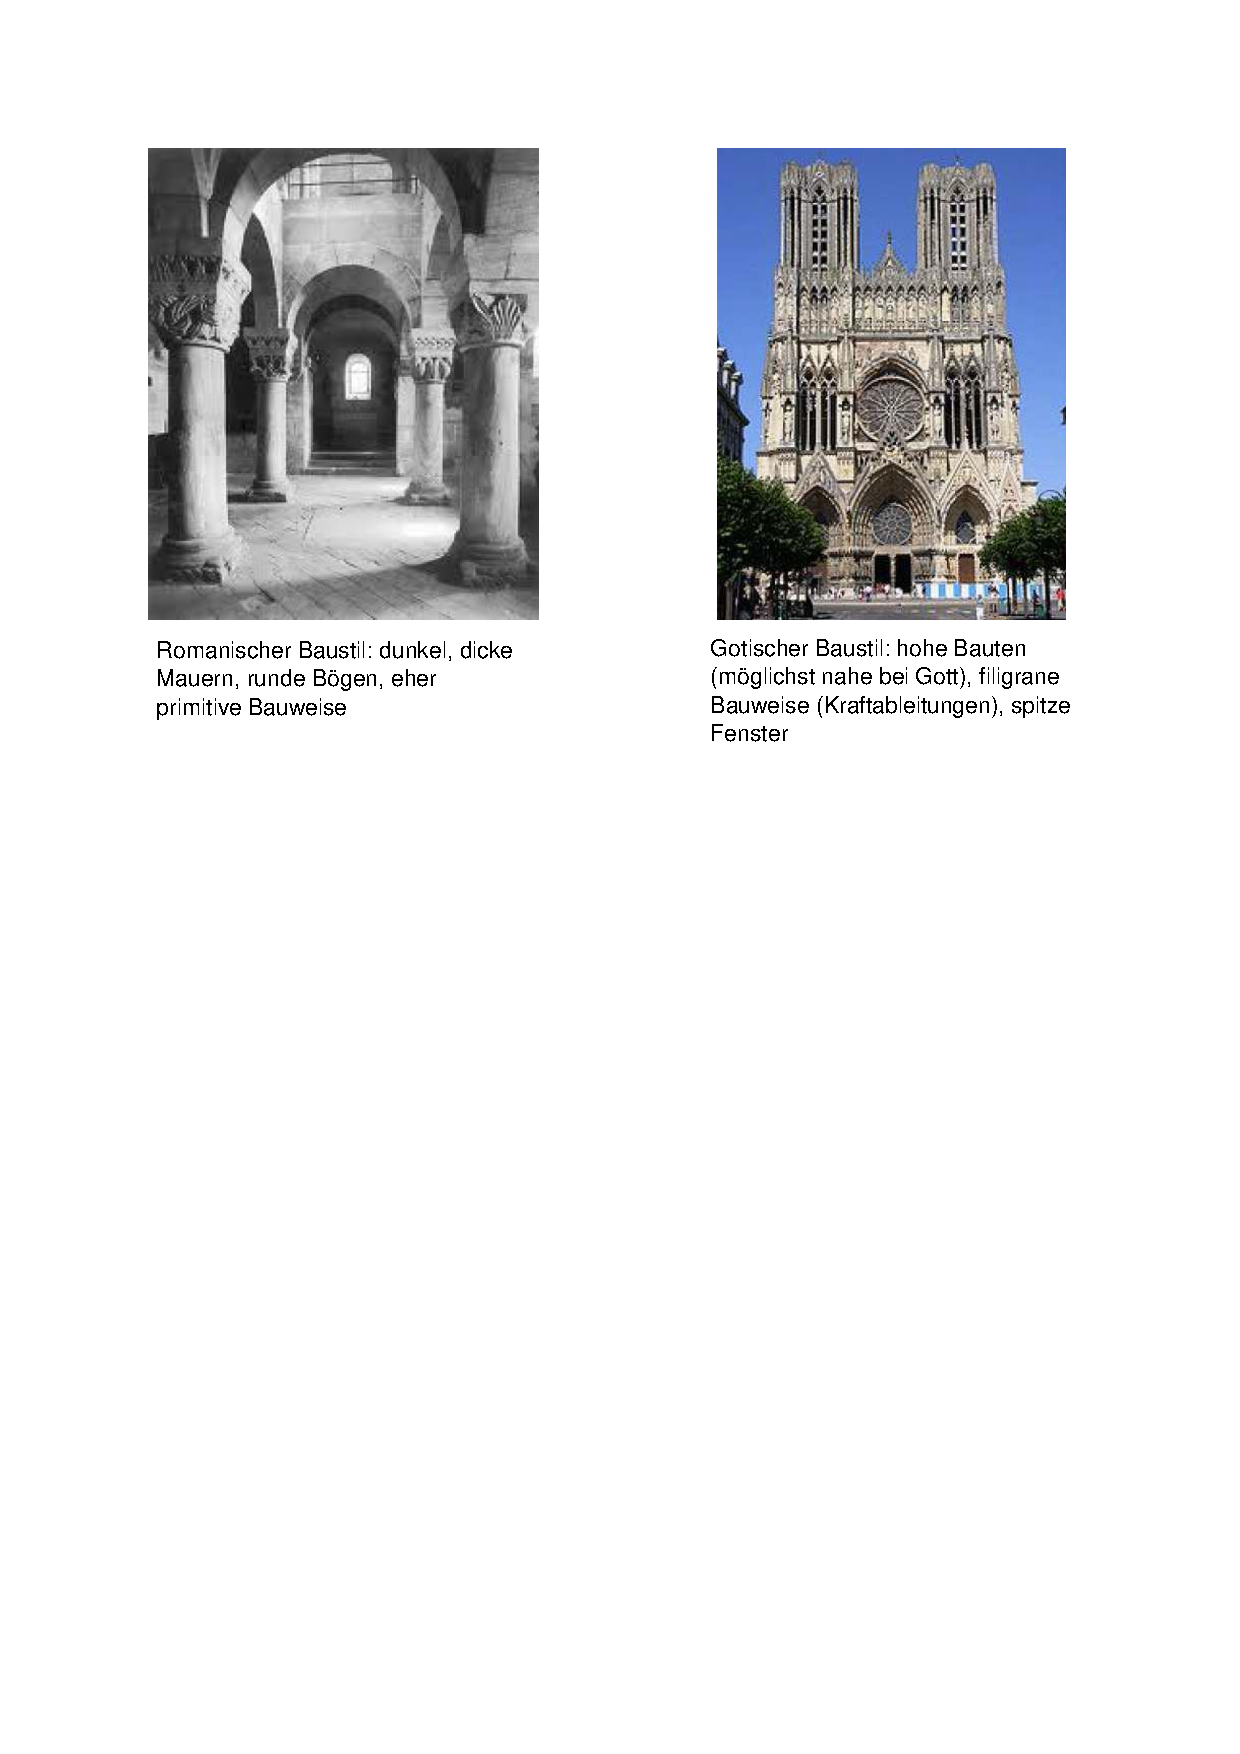
\includegraphics[width=.8\textwidth]{images/Baustil1}
\subsubsection{Mittelalter - Zeit der Zünfte}
Gewerbe – Handel (reichste) – Landwirtschaft\\
Zünfte = städtische Berufsgenossenschaften\\
Um die Nahrungssicherheit zu bekommen findet eine Monopolisierung des gewerblichen Wissens und der gewerblichen Tätigkeit statt. Zünfte beginnen ihre Bereiche selber zu regeln. Werden zu einer politischen und militärischen
Organisation. Bruch der Herrschaft der Fürsten – Ende des Feudalismus. \glqq Stadtluft macht frei! \grqq Es entsteht ein Lohnverhältnis zwischen Meister (Zünftler) und Arbeiter. Organisation der Berufsbildung (Gesellen / Lehrling, Lehrzeit, Prüfung, Wanderschaft – Meisterprüfung)
\subsection{Renaissance – Zeit des Aufbruchs}
1436 Erfindung des Buchdruckes und 1500: 27'000 Werke mit einer Auflage von 20 Millionen erschienen. Wissen wurde dank den Büchern kauf- und transportierbar. Es fanden Entdeckungsreisen statt, mit den Folgen, dass Lebensmittel importiert wurden (Kakao, Tabak, Tomaten, Mais und Kartoffeln), die Übertragung von Krankheiten anstieg, die Wirtschaft globalisiert wurde und Leute begannen in ein anderes Land auszuwandern (neues Weltbild)
\subsubsection{Neue Bauten, neue Malerei}
Anders als im Mittelalter steht man zu seiner Macht. Man fühlt sich gleich mächtig wie Gott. Schönheit wird nicht mehr als Werk Gottes angesehen sondern als Werk der Natur. Künstler beginnen ihre Werke zu signieren.\\
Leonardo da Vinci (1452 - 1519): ein \glqq Genie \grqq, Künstler, Architekt, Musiker, Wissenschaftler, Mediziner, Geologe, Zeichner, Maler und Erfinder\\
Bauten: Man baute breit und nicht mehr hoch um nahe bei Gott zu sein. Man will seine Macht durch die Grösse der Bauwerke zeigen. 

\subsection{Reformation - ab 1517}
Man gelangt zu der Ansicht, dass wenn man viel Arbeitet man dankbar ist. Reformation durch: Luther in Deutschland, Zwingli und Calvin in der Schweiz. Die Arbeit wird ein zentrales moralisches Element des Lebens (Arbeit macht Freude). Die Arbeit wird als Anerkennung Gottes und als Geschenk Gottes angesehen (doppelte Prädestination). Die Bibel als einzige göttliche Wahrheit $ \rightarrow $ Alle sollten sie lesen können $ \rightarrow $ Allgemeine Schulpflicht wird eingeführt. Der Reichtum ist kein Laster, sondern ein Zeichen Gottes, sofern man damit anständig umgeht (nicht angeben). Zinsen- und Bankgeschäfte werden Christen erlaubt. Erste Privatbankiers (haften mit Privatvermögen) in Genf, Basel und St.Gallen. Keine Dogmen – mehr Forschungen werden toleriert. Grosse Religionskriege in Europa bis 1648
\subsubsection{500 Jahre Reformation – Die Aktualität reformatorischen Denkens}
\begin{citemize}
	\item Grundlegende Neuordnung von Kirche, Politik, Gesellschaft und Wirtschaft
	\item Hoher Stellenwert der Bildung
	\item Fundament für Rechtsstaat und Menschenrechte $ \rightarrow $ Freiheit des Einzelnen
	\item Eigentum und gerechte Verteilung
	\item Soziale Sicherheit
	\item Erfolgreiche Schweizer Entwicklung (Kein Stadt-Land-Gegensatz $ \rightarrow $ Zusammenhalt)
\end{citemize}
\subsection{Ancien Regime – Absolutismus ab 1661}
\begin{citemize}
	\item Anti-freiheitliche Welle – absolutistische Monarchien (Bsp. König Ludwig XIV)
	\item Keine Anwendungen von neuen Erfindungen
	\item Wirtschaft wird vom \textbf{Merkantilismus} dominiert: (Handwerk, Verlagswesen (Heimarbeit) und Manufakturen)
	\item Wissenschaft macht in Grossbritannien grosse Fortschritte
	\item Die neuen wissenschaftlichen Erkenntnisse werden zuerst in Grossbritannien wirtschaftlich nützlich angewendet.
	\item Merkantilismus: unser Staat reich, Nachbar arm
	\item Rohstoff Export schlecht $ \rightarrow $ Rohstoff Import + Produktion + Produkt Export $ \rightarrow $ viel Geld
	\item Barock = Stil der Gemälde und Bauten während des Absolutismus \vspace{0.5cm}
\end{citemize}
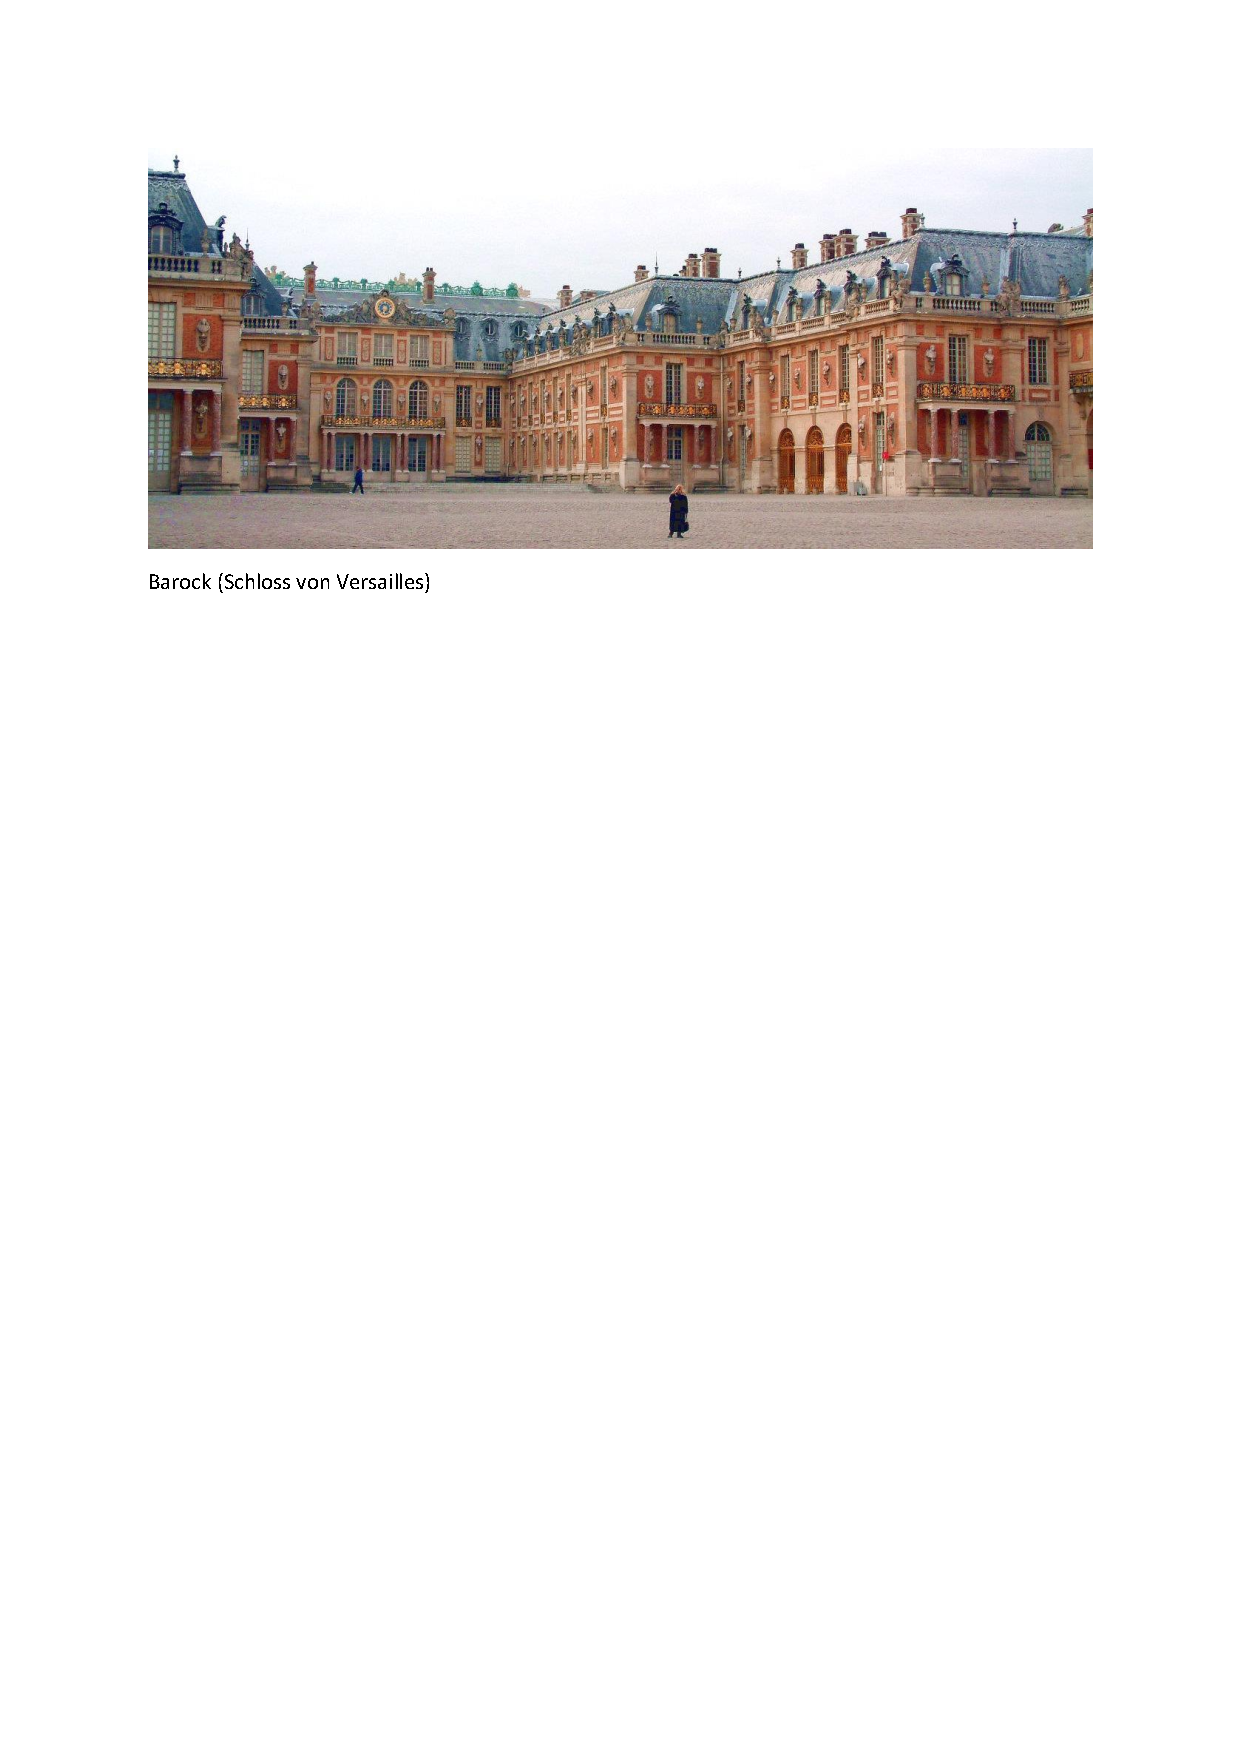
\includegraphics[width=1\textwidth]{images/Barock}
\clearpage
\section{Industrielle Revolution}
\subsection{Geistige Voraussetzungen}
\subsubsection{Die Aufklärung}
Geistige Bewegung aus dem 18. Jahrhundert, die die Vernunft als Prüfstein der Wahrheit betrachtet. Alles was nicht rational begründet werden kann, wird als Vorurteil oder Aberglaube abgelehnt. Der Mensch als vernünftiges Wesen kann die Vernunft als Richtschnur für sein Leben anwenden. Wir handeln jedoch unvernünftig, wenn Gefühle ins Spiel kommen. Daher ist der Mensch mit Rechten auszustatten. Aufklärer waren skeptisch, rationalistisch und optimistisch. \glqq Cogito ergo sum \grqq – ich denke also bin ich. I. Kant: \glqq Aufklärung ist der Ausgang des Menschen aus seiner selbstverschuldeten Unmündigkeit. Unmündigkeit ist das Unvermögen, sich seines Verstandes ohne Leitung eines anderen zu bedienen.\grqq  Hinterfragen heisst, dass man ein Mensch ist. 
\subsubsection{Staatstheorie John Locke (1632 - 1704}
Der Mensch wird frei und vernünftig geboren. Menschen haben einen Gesellschaftsvertrag geschlossen, um einen Staat zu bilden. Aber nicht nur der Mensch hat gegen über dem Staat Pflichten, sondern auch der Staat ist gegenüber dem Menschen verpflichtet. Er muss ihn schützen und ihm durch die Natur zugestandene Rechte (Recht auf Leben, Recht auf persönliche Freiheit, Eigentumsgarantie, usw.) gewähren. Der Mensch hat ein Widerstandsrecht gegenüber Herrschern, die ihren Verpflichtungen nicht nachkommen. John Lock hatte als erster die Gewaltentrennung im Sinne. Verschiedene Staaten versuchten mehr oder weniger die Ideen zu übernehmen (1. USA, 2. Schweiz)
\subsubsection{Empirismus John Locke}
Ursprung jeder Erkenntnis liegt in der Erfahrung. Wissen entsteht aus der Sinneswahrnehmung. Durch logische Auswertung können Erkenntnisse über Gegenstände gewonnen werden, die der direkten Sinneswahrnehmung entzogen sind. Der Empirismus führt zu einem Schub der Naturwissenschaften, da man neue Antworten auf neue Fragen erhält. Mikroskope wurden in dieser Zeit entwickelt.
\subsubsection{Aufklärung und Naturwissenschaften}
Bereits im 17. Jahrhundert waren die Grundlagen der mechanischen Physik und der Mathematik gelegt worden. Die Denk- und Arbeitsweisen der Aufklärung wirkten sich fruchtbar auf die Naturwissenschaften aus. Dies betraf vor allem die Elektrizitätslehre, die Wellentheorie des Lichtes, die wissenschaftliche Chemie und die systematische Biologie und Zoologie. In der Aufklärung wurden die mathematisch formulierten Naturgesetze erstmals für praktische
Bedürfnisse angewendet. Als grosse Hilfe dienten dabei die in der Aufklärung entwickelten genaueren Messinstrumente. 
\subsubsection{Physiokratismus}
Lehnte den Merkantilismus ab. War überzeugt, dass nicht eine aktive Handelsbilanz, sondern die Urproduktion (Landwirtschaft und Bergbau) zu einer Vergrösserung des Volkswohlstandes führt. Gaben die Anstösse zur Agrarrevolution. Physokraten glauben Vermögen kommt aus dem Boden (zB. Landwirtschaft). Dies führte dazu, dass die Kartoffel zum Grundnahrungsmittel wurde.
\subsubsection{Klassische Nationalökonomie}
Adam Smith veröffentliche 1776 \glqq Die Volkswohlfahrt \grqq . Auch die Wirtschaft folgt einfachen Gesetzen. Antriebsfeder ist dabei dem Menschen sein eigener Vorteil (Jeder möchte möglichst viel Gewinn machen). Wenn jeder für sich schaut – geht es allen besser. Daher freie Marktwirtschaft und keine staatlichen Eingriffe ins Wirtschaftsleben. Arbeitsteilung führt zu grösserer Produktivität (Jeder soll produzieren was er gut kann). 
\subsection{Bevölkerungswachstum}
Die Bevölkerung in Europa nahm im 18. Jahrhundert von 120 auf 190 Millionen zu. Frauen hatten um die 18 Kinder jedoch überlebten meist nur etwa 3. Zwischen 1800 und 1900 verdoppelte sich die europäische Bevölkerung nochmals, obwohl mehrere Millionen nach Amerika auswanderten. In der Schweiz war die Bevölkerung 1700 1.2 Millionen, 1800 1.8 Millionen und 1900 3.3 Millionen gross. Die Geburtenrate blieb gleich, jedoch sank die Sterberate, vor allem durch die tiefere Säuglingssterblichkeit (Medizinischer Fortschritt, Verbesserte Hygiene, Agrarrevolution).
\subsection{Die Agrarrevolution}
Trockenlegung von Sumpfgebieten (Bsp.: Linthebene mit Linthkanal) führt zu grösseren Landwirtschaftsflächen. Ende der Dreifelder-Wirtschaft und Einführung der Fruchtwechsel-Wirtschaft. Aufteilung der Allmen unter den Bauern. Bau von Jauchegruben. Einführung der Sommer-Stallfütterung führte zu 20\% mehr Futterertrag. Einführung der Blattfrüchte Klee, Kartoffel und Zuckerrübe. Durch den Kleeanbau wurde der Boden auf natürliche Weise mit Stickstoff gedüngt. Mechanisierung durch verbesserten Pflüge, Eggen, Mähmaschinen und Heuwender. Einsatz von Kunstdünger (Stickstoff und Phosphate) ab 1850. Vorher Import von Chilesalpeter (Vogeldreck aus Chile). Züchtung von Pflanzen und Tieren, gemäss der Vererbungslehre von Darwin und Mendel. Rationalisierung der Viehhaltung. Das Schwein wird vom Weidetier zum Stalltier. Abgabe von Kraftfutter. Mehr Fleischkonsum führte zur besseren Gesundheit der Bevölkerung. Der Mensch ist ein Allesfresser und verzichtet nur aus moralischen Gründen auf gewisse Dinge.
\subsection{Wissenschaftliche Veränderungen}
Wissenschaftliche Entdeckungen wurden erst umgesetzt, wenn ein Bedarf für ihren Einsatz und das Kapital vorhanden war. Beispiel der Textilindustrie mit drei technisch überwundenen Engpässen:\\ \\
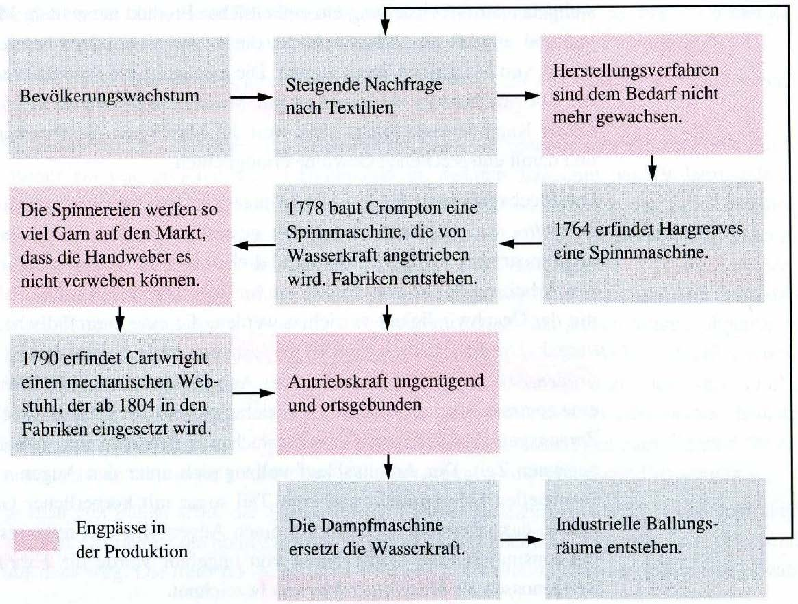
\includegraphics[width=.8\textwidth]{images/textil_1}
\subsection{Kapital}
Mit der Industriellen Revolution war der Kapitalbedarf viel grösser geworden. Dies aus zwei Gründen:\\
1. Erstausrüstung der Fabrik und laufende Erneuerung\\
2. vermehrte Aufwendungen für Rohstoffe, Löhne und Energie\\
Woher kam das notwendige Kapital? Dazu gibt es verschiedene Theorien: Von der wegen der Agrar-Revolution prosperierenden Landwirtschaft. Gewinne aus dem Fernhandel, speziell des Kolonialhandels. Individuelle Ersparnisse des Unternehmers und seiner Verwandtschaft. Sobald der Industrialisierungsprozess in Gang gekommen war, erzeugte dieser das nun benötigte Kapital selber.
\subsection{Neue Einstellung zur Arbeit}
Das vor-kapitalistische Ideal des \glqq gerechten Preises \grqq wird durch die Gewinnmaximierung ersetzt. Alles hat seinen Preis, auch die Arbeit. Durch den freien Arbeitsmarkt, speziell in Grossbritannien, konnte der ländliche Bevölkerungsüberschuss in die Fabrikstädte strömen. Der wirtschaftliche Freiraum wurde, speziell in Grossbritannien, immer grösser. Wichtige Entwicklungen waren die Eigentumsgarantie, die vom Unterhauses, das vom Bürgertum dominiert wurde, reduzierte Steuer- und Abgabenbelastung und die sukzessive Aufhebung der Zunftordnung. Die Puritaner (englische Reformierte) sahen im materiellen Reichtum ein Zeichen der besonderen Gnade Gottes. Die ersten industrialisierten Gebiete Europas waren mehrheitlich von Protestanten bewohnt. In England durfte erst wählen, wer ein gewisses Vermögen besass. In das Parlament konnten nur Personen mit sehr grossem Vermögen. Auch Adlige arbeiten in GB, da sie ebenfalls Reformierte sind.
\subsection{Industrialisierung: Textilindustrie}
\subsubsection{Die vier Arbeitsschritte bei der Textilherstellung}
\begin{enumerate}
\item Das Rohmaterial muss sortiert, gereinigt, egreniert (Samen und Faser trennen (Baumwolle)) und gekämmt werden.
\item Die losen Fasern werden verzogen und zu einem Faden gezwirnt. Der gesponnene Faden wird Garn genannt.
\item Das Garn wird gewoben. Durch längs und quer gespannte Garnfäden entsteht ein Gewebe.
\item Letzter Arbeitsgang ist das Appretieren, bestehend aus dem Walken, Reinigen, Scheren, Färben, Bedrucken und Bleichen
\end{enumerate}
\subsubsection{Chronologischer Ablauf der technischen Entwicklung}
\begin{tabularx}{1\textwidth}{L{3cm}  X}
\rowcolor[gray]{.6} \textbf{Jahr} & \textbf{Entwicklung} \\ 
1764 & J. Hargreaves baut eine Baumwollspinnmaschine (Spinning Jenny)\\
\rowcolor[gray]{.9} 1769 & Richard Arkwright betreibt die erste mit Wasserkraft betriebene Spinnmaschine \\
1784 & Edmund Cartwright baut den ersten mechanischen Webstuhl\\
\rowcolor[gray]{.9} 1785 & Erste mit Dampfkraft angetriebene Baumwollspinnerei\\
1807 & Erstes Dampfschiff\\
\rowcolor[gray]{.9} 1830 & Eröffnung der Eisenbahnlinie Manchester – Liverpool\\
1866 & Siemens erfindet den Dynamo für Starkstrom\\
\rowcolor[gray]{.9} 1885 & Daimler und Benz bauen Benzinmotoren in Fahrzeuge ein\\
\end{tabularx}
\subsection{Industrialisierung: Grossbritannien}
\subsubsection{Besondere Voraussetzungen}
Geographische Lage (Insel und viele schiffbare Flüsse) war optimal. Grossbritannien verfügt über die grösste Handelsflotte und die Royal Navy schützt die Insel. Optimale Voraussetzungen für den weltweiten Zugang zu Rohstoffen und Absatzmärkten zudem gab es keine Binnenzölle. Durch die Religionspolitik von König Heinrich VIII und der Königin Elisabeth I lebten drei Kirchen friedlich miteinander (Anglikanische Staatskirche, Katholische Kirche und die protestantischen Kirchen. Seit der Glorreichen Revolution von 1689 ist Grossbritannien eine konstitutionelle Monarchie. Parlament entscheidet über Gesetze und Steuern. Durch das Zensuswahlrecht wird das Parlament von unternehmerisch tätigen Männern dominiert. Der König darf keine Armee unterhalten. Im Gegensatz zu Kontinentaleuropa ist der Adel wirtschaftlich tätig. Konzentration in der Landwirtschaft ab Mitte 17. Jahrhundert. Die Kleinbauern wurden zu Landarbeitern – die grossen Höfe rationalisierten und produzierten für die Städte. Viele Landarbeiter verloren in der rationalisierten Landwirtschaft ihre Arbeit und begannen in die Städte abzuwandern. Unternehmer gingen in die Schweiz, weil hier die Löhne noch tiefer waren (Brown Boveri) London 1800: 1 Million Einwohner und die grösste Stadt Europas. Ausbau der Wasserwege und der Strassen im 18. Jahrhundert. Kein Punkt ist mehr als 100 Km vom Meer entfernt. Wegen dem Schiffsbau, Holz als wichtigsten Energielieferant und der Eisenverhüttung durch Holzkohle war Grossbritannien fast völlig entwaldet. In der ersten Hälfte 18. Jahrhundert gelang es der Steinkohle Gas zu entziehen und Koks als veredelte Kohle bei der Eisenverhüttung einzusetzen. Die sich an der Erdoberfläche befindlichen Kohlevorkommen erschöpften sich im Laufe des 18. Jahrhunderts. Mit Pumpen musste das Grundwasser aus den immer tiefer gegrabenen Schächten abgepumpt werden.
\subsubsection{Ablauf der Industriellen Revolution in Grossbritannien}
Wer \glqq industrielle Revolution \grqq  in Grossbritannien sagt, sagt Baumwollindustrie. Um 1700 waren die Engländer führend in der Wollstoffherstellung und das Baumwollgewerbe steckte erst in den Anfängen. Um die grossen Schafzüchter zu schützen, verbot die Regierung die Einfuhr von Wolle. Die Textilhersteller bei den Kolonialhäfen wichen daher auf die Baumwollverarbeitung aus. Zu dieser Zeit begann man auch Unterwäsche zu tragen. Im Siebenjährigen Krieg (1756 – 1763) konnte Grossbritannien Frankreich aus Indien vertreiben und zwang darauf die Inder britische Baumwollstoffe zu importieren. Die indische Baumwollindustrie wurde zerstört. Grossbritannien förderte den Baumwollanbau in seinen südlichen Kolonien in Nord-Amerika. Durch den Sklavenhandel profitierte Grossbritannien in dreifacher Weise. Neben dem reinen Gewinn des Sklavenhandels, wurde durch die Sklaven die Produktion von Baumwolle billiger und in Afrika tauschten die Händler Baumwollprodukte gegen Menschen ein. \textbf{(Dreieckshandel Europa - Afrika - Amerika)} Der eigentliche Engpass bildete den aufwendigsten Arbeitsprozess, das Spinnen. Ein Weber konnte die Arbeit mehrerer Spinnerinnen verarbeiten. 1764 konnte James Hargreaves mit der \glqq  Spinning Jenny \grqq eine Maschine konstruieren, bei der zuerst 8, dann später gleichzeitig 16 Spindeln von Hand angetrieben werden konnten. Richard Arkwright betrieb die erste durch Wasserkraft angetriebene Spinnmaschine. 1778 baute Samuel Crompton die \glqq  Mule-Jenny \grqq, eine mit Wasserkraft angetriebene Spinnmaschine mit bis zu 50 Spindeln. Dadurch wurde nun mehr Garn hergestellt, als die Weber verarbeiten konnten. 1784 konnte der Pfarrer und Erfinder Edmund Cartwright den mechanischen Webstuhl konstruieren. Die Textilindustrie war nun industriell umgestellt. Die Textilindustrie befand sich jedoch immer noch an den Flüssen. Diese Flüsse mussten aber über regelmässige Wasserführung und über eine genügend starke Steigung verfügen. (Die Schweiz wurde daher als 2. Gebiet in Europa industrialisiert). Vor allem das Glarnerland wurde für seine Stoffe weltbekannt. Ab 1785 wurde somit die von James Watt entwickelte Dampfmaschine als Antrieb für die Maschinen verwendet.\\ \\
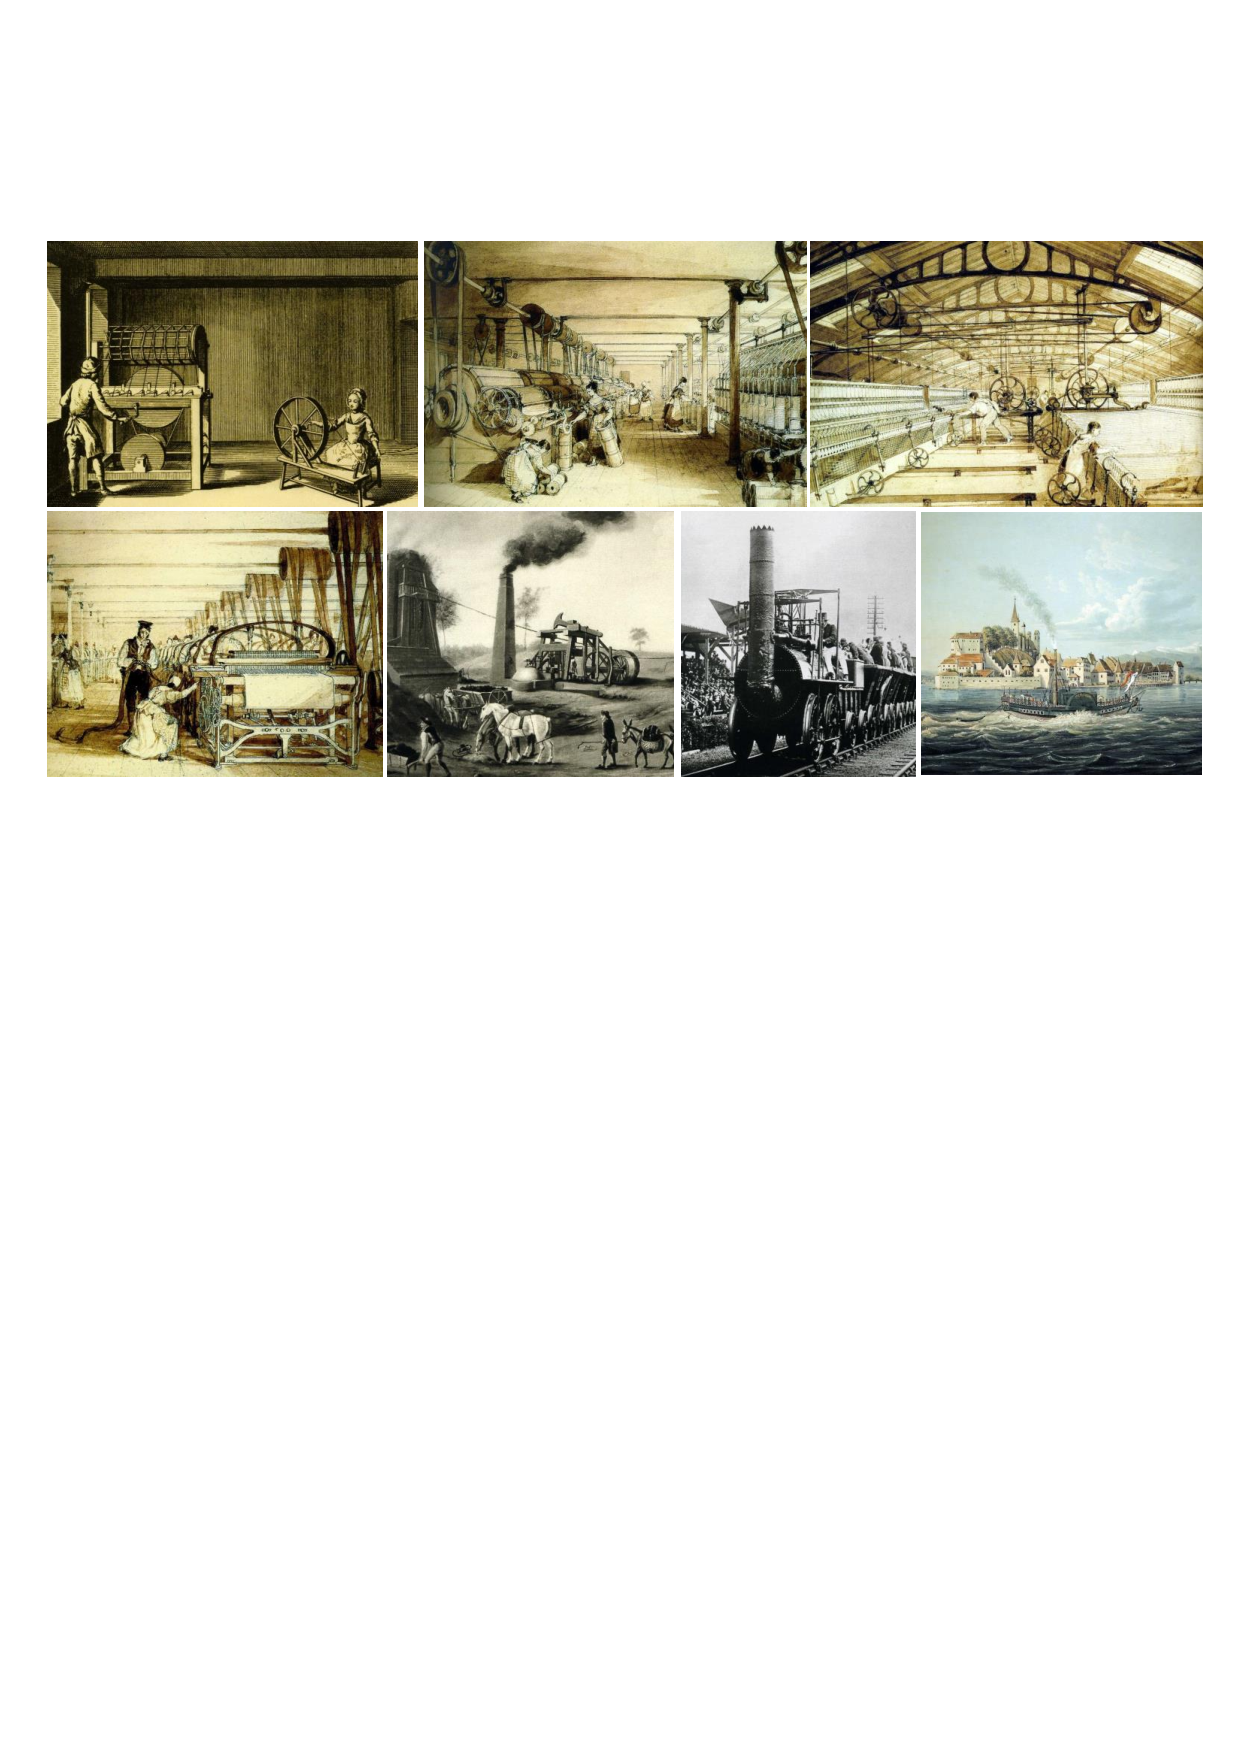
\includegraphics[width=1\textwidth]{images/maschinen}
\clearpage

\section{Die Zweite industrielle Revolution}
Zwischen 1815 bis 1830 erschwert das konservative politische Umfeld in Europa die Industrialisierung. Durch die Erfolge der liberalen Bewegung in vielen Ländern ab 1830 beschleunigte sich die Industrialisierung, speziell in Frankreich und Belgien. Später fanden Industriellen Revolutionen auch in Deutschland und den USA (1861 – 1865 Bürgerkrieg) statt. Die Dominanz Grossbritanniens ging langsam zurück. Als neue aufstrebende Industrienationen positionieren sich Deutschland (\glqq Made in Germany\grqq ) und die USA. Ab 1870 kann von einer Weltwirtschaft gesprochen werden. Der wirtschaftlich immer engeren Zusammenarbeit standen politisch gegensätzliche Bestrebungen entgegen, die schliesslich in den Ersten Weltkrieg führen sollten.
\subsection{Stahl-, Elektro-, Chemie- und Verkehrs-Industrie}
Zwischen 1870 und 1880 fanden viele herausragende Erfindungen auf den Gebieten Physik und Chemie statt.
\subsubsection{Eisen- und Stahlindustrie}
Es gelang nun mit der Bessemerbirne, dem Martin-Siemens-Verfahren (Stahlherstellung aus Schrott) und dem Thomas-Verfahren (Verarbeitung von phosphorhaltigem Eisen) Stahl viel günstiger herzustellen und voluminöse Stahlstücke zu giessen. Dies ermöglichte einen massiven Ausbau von Eisenbahnlinien: \textit{Brennerbahn 1867, Central Pacific 1869, Mont-Cenis-Bahn 1871, Gotthardbahn 1882, Northern Pacific und Southern Pacific 1883, Transsibirische Eisenbahn 1900}
\subsubsection{Elektrotechnische Industrie}
1866 entdeckt Werner von Siemens das elektrodynamische Prinzip (Prinzip der Selbsterregung) und darauf Bau des ersten Gleichstromgenerators. 1878 entwickelt von Siemens den zweipoligen Dynamo – später Bau von Wechselstromgeneratoren. 1879 entwickelt Edison die Kohlenfaden-Glühlampe.
\subsubsection{Chemische Industrie}
Ab 1860 Produktion von Anilin- und Teerfarben, von Medikamenten und von Kali- und Stickstoffdünger. Ab 1880 Gewinn von Metall durch die Elektrolyse und ab 1890 Produktion von Schwefelsäure.
\subsubsection{Motorenindustrie und Verkehrswesen}
1824 erste Lokomotive \glqq Rocket\grqq von Stephenson. In den 1830er Beginn des Eisenbahnbaus in Grossbritannien und in den 1840er Beginn des Eisenbahnbaus in Kontinental-Europa. 1860 braucht ein Schraubendampfer noch 24 Tage für die Atlantiküberquerung. Ab 1870 massiver Eisenbahnbau dank billigem Stahl. 1883 erstes Patent für einen Benzinmotor und 1885 erster Benzinmotor von Benz. 1893 erster Dieselmotor. 1910 braucht ein Turbinendampfer noch 8 Tage für die Atlantiküberquerung.\\
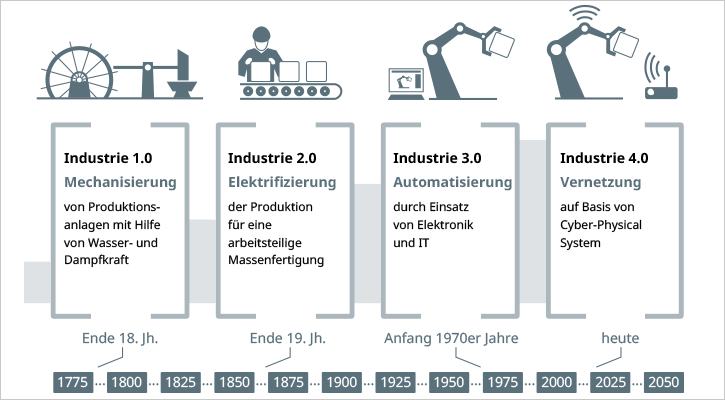
\includegraphics[width=.65\textwidth]{images/Industrieentwicklung}
\subsection{Die Soziale Frage}
Als Soziale Frage wird die materielle und rechtliche Situation der Arbeiterschaft vor allem während der zweiten Industriellen Revolution verstanden. Dabei geht es in erster Linie um die Frage: \vspace{0.25cm}
\begin{citemize}
\item Die Aufteilung der Gesellschaft statt nach Ständen nach Klassen (Bürgertum / Bourgeoisie – Arbeiter / Proletariat)
\item Die Verkleinerung des handwerklich – gewerblichen und des heimwerklichen Teils in der Wirtschaft
\item Die materiellen Arbeitsbedingungen der Arbeiter
\item Die rechtlichen Arbeitsbedingungen der Arbeiter
\item Frauen- und Kinderarbeit
\item Wohnsituation \vspace{0.25cm}
\end{citemize}
\subsubsection{Die materiellen Arbeitsbedingungen der Arbeiter}
Feuchte, dreckige und gefährliche (Transmissionsriemen) Arbeitsplätze. Lange Arbeitstage (bis zu 16 Stunden) während einer 6 Tage Woche. Keine Ferien, keine Weiterbildung und keine Freizeit. Drakonische Strafen für Zuspätkommen und für Fehler bei der Arbeit. Akkordlöhne waren Reproduktionskostenlöhne (deckten gerade die Existenzbedürfnisse). Teilweise wurde sogar nach dem Trucksystem (mit Ware (Gutscheine für Fabrickladen), in der Schweiz heute verboten) entlöhnt. Viele Frauen und Kinder wurden angestellt, da diese billiger waren. Wie konnten die Heimarbeiter, Handwerker und das Gewerbe überleben? Fabrikbrand von Uster 1832 oder die Zerstörungen von Maschinen; Todesstrafe in Grossbritannien für die Maschinenstürmer.
\subsubsection{Die rechtlichen Arbeitsbedingungen der Arbeiter}
Es gab keine unbefristeten Arbeitsverträge. Die Arbeiter hatten Pflichten gegenüber dem Arbeitgeber, umgekehrt jedoch nicht. Es gab keine Unfall-, Kranken-, Alter- oder Arbeitslosenversicherung. In der Schweiz gab es zusätzlich keine Arbeitsplatzgarantie bei Militärdienst! Durch die Fabrikläden und die Mietskasernen der Unternehmer konnten die Arbeiter noch mehr an das Unternehmen gekettet werden.
\subsubsection{Frauen und Kinderarbeit}
Frauen hatten die schlechteren Arbeiten zu leisten und wurden weniger bezahlt. Keine Frau konnte Vorgesetzte von Männern sein. Frauen hatten eine Doppel- teilweise Dreifach-Belastung gegenüber den Männern. Frauen arbeiteten bis zur Niederkunft, teilweise gebaren sie in der Fabrik. Mütter erschienen nach der Niederkunft möglichst schnell wieder in der Fabrik – Säuglinge wurde mit Schnaps ruhiggestellt. Sobald Kinder eine Arbeit ausführen konnten, arbeiteten sie in der Fabrik. Kinder arbeiteten in der Nacht um am Tag der Schulpflicht nachzukommen zu können - Armutsteufelskreis! Bis 1842 fast 50\% der Fabrikarbeiter unter 16 Jahre alt.
\subsubsection{Wohnsituation}
Wohnungen werden Spekulationsgut. Wegen den Windverhältnissen in Europa soziale Aufteilung der Städte (Aufteilung der Stadt so, dass dreckige Luft nur in den Industrie- und Arbeitervierteln. Grosse Alleen für Durchlüftung der Stadt und zur einfachen Bekämpfung von Aufständen.) Quartiere werden umgebaut um Revolten zu verhindern (Boulevard in Paris).
\subsubsection{Technische Entwicklung führt zu einer Verbesserung der Situation der Arbeiter}
Anspruchsvollere Maschinen verlangen ausgeruhte und ausgebildete Arbeiter. Die Ausbildung der Arbeiter kostet Geld, was dazu führt, dass die Arbeitszeit gesenkt wird und die Löhne erhöht werden (eine Ausbildung kostet den Arbeitgeber). Arbeitgeber bieten Hobbys und Ablenkungsmöglichkeiten, denn Glückliche Arbeiten leisten bessere Arbeit und sind produktiver. Das zusätzliche Geld und die nun vorhandene Freizeit führt zur Vergrösserung von 2 Problemen: Alkoholismus und Prostitution (Krankheitsübertragung durch Prostitution (Syphilis))
\subsection{Lösungen der Sozialen Frage}
Durch die technische Entwicklung (Fortschritte) verkleinert sich die Soziale Frage, da anspruchsvolle Maschinen gut ausgebildete und ausgeruhte Arbeiter verlangt.\\
\begin{tabularx}{1\textwidth}{L{3cm} L{4cm}  X}
\rowcolor[gray]{.6} \textbf{Wer?} & \textbf{Wieso?} & \textbf{Wie?}\\ 
Arbeiter & Selbsthilfe & Parteien \newline Gewerkschaften \newline Streiks(Arbeitervereine)\\
\\
\rowcolor[gray]{.9} Unternehmer \newline (Arbeitgeber) & Soziale Gesinnung \newline Angst vor Aufständen & Schulen \newline Wohnungen \newline Krankenhäuser \\
\\
Staat & Sozialer Friede \newline Angst vor Aufständen \newline Allgemeine Wehrpflicht & Soziale Gesetzte 
\begin{citemize} 
\item Arbeitszeit 
\item Versicherungen 
\end{citemize}
 Koalitionsrecht \newline Senkung Zölle 
\begin{citemize} 
\item Billigere / Bessere Ernährung 
\item Löhne senken 
\item Produktion / Produkte billiger 
\item Exporte verbessern 
\end{citemize}\\
\rowcolor[gray]{.9} Kirchen & Nächstenliebe \newline Säkularisierung & Heilsarmee, Hilfswerke \newline Gaststätten, Heime\\
\\
Philosophen & Bessere Welt & Neue Philosophien / Ideologien \newline Sozialismus\\
\end{tabularx}
\subsubsection{Die Genossenschaftstheorie - Robert Owen (1771-1858)}
\begin{wrapfigure}[6]{r}{2cm} 
\vspace{-0.5cm}
  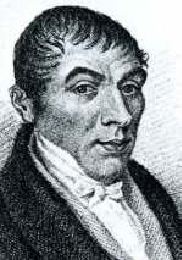
\includegraphics[height=2.5cm]{images/owen}
\end{wrapfigure}
Das Unternehmen gehört den Arbeitern. Somit bekommen die Arbeiter den von ihnen produzierten Mehrwert. Das Verhältnis zu ihrer Arbeit verändert sich. Demokratischere Wirtschaft. In Frankreich 1848 die Idee von genossenschaftlich- staatlichen Nationalwerkstätten umgesetzt. Genossenschaften können günstiger produzieren, somit werden langfristig durch die Konkurrenz die privaten Unternehmen untergehen. Friedlicher Weg in den Sozialismus. Beispiele: Coop, Mobiliar, Baugenossenschaften – nicht die Migros!
\subsubsection{Die Staatssozialistische Theorie - Claude de Saint-Simon (1760 - 1852)}
\begin{wrapfigure}[6]{r}{2cm} 
\vspace{-0.5cm}
  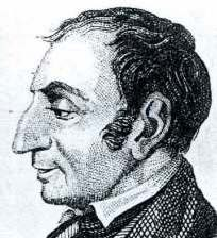
\includegraphics[height=2.5cm]{images/declaude}
\end{wrapfigure}
Theorie: Das Hauptproblem ist die Produktion von Massengütern. Leitspruch daher: Alles durch und für die industrielle Produktion. Der Staat soll die Wirtschaft planen. Politiker sollten ihre Macht Wirtschaftsführern mit einem sozialen Gewissen übergeben. Bau um den Transport zu verbilligen (Bau von Kanälen) und Binnenmärkte (europäischer Wirtschaftsmarkt) schaffen. In der Schweiz ist die Landwirtschaft so gelöst und der ÖV (SBB) sowie die Post. Den Leuten geht es schlecht, weil es zu wenig Güter hat. 
\subsubsection{Die Anarchistische Theorie - Michael Bakunin (1814-1876)}
\begin{wrapfigure}[6]{r}{2cm} 
\vspace{-0.5cm}
  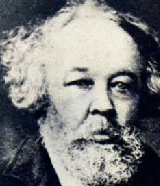
\includegraphics[height=2.5cm]{images/bakunin}
\end{wrapfigure}
Hauptübel ist die Herrschaft von Menschen über Menschen. Dies ermöglicht der Staat. Abschaffung des Staates um den Menschen sowohl von der wirtschaftlichen als auch von der staatlichen Gewalt zu befreien. Zwei Strömungen innerhalb der Bewegung: der gewaltlose Weg und die Befürwortung der gewaltsamen Vernichtung des Staates (Massensterben von Staatsoberhäuptern durch Anarchisten). Dem Menschen geht es schlecht weil sie vom Staat \glqq unterdrückt\grqq werden.
\subsubsection{Die Marxistische Theorie - Karl Marx (1760 - 1825)}
\begin{wrapfigure}[7]{r}{2cm}
\vspace{-0.5cm} 
  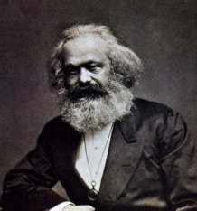
\includegraphics[height=2.5cm]{images/marx}
\end{wrapfigure}
Die Analyse der Situation in Grossbritannien in den 1840er ist richtig – mit dieser Analyse versucht er die ganze Weltgeschichte zu erklären (Historischer Materialismus)
Theorie 1: Mehrwerttheorie (Steigerung des Wertes der Arbeit (Der Lohn wird immer tiefer sein als der Wert der Arbeit))\\ Theorie 2: Verelendungstheorie (Arbeitgeber möchte immer weniger bezahlen) \\ Theorie 3: Konzentrationstheorie (Fusion von Konkurrenten) \\ Theorie 4: Entfremdungstheorie (Keine Emotionale Beziehung zum Produkt, kein Bezug mehr)\\
Diese Theorien wurden bis ca. 1990 von 2/3 der Menschheit als richtig angesehen.
\section{Wir wollen uns bewegen – Entwicklung der Verkehrsmittel}
\begin{tabularx}{1\textwidth}{L{2cm} L{4cm} L{3cm} X}
\rowcolor[gray]{.6} \textbf{-} & \textbf{Wer} & \textbf{Epoche} & \textbf{Transporttechnik}\\ 
6.1 & Pilger, Händler, Krieger \newline (Römische Händler ohne Söldner unterwegs) & Antike bis ca. 1450 & Fuss, Schiff, Wagen\\
\rowcolor[gray]{.9} 6.2 & Entdeckungsreisende & 1450 bis 1800 & Schiff, Fuss\\
6.3 & Bildungsreisende & 1600 bis 1914 & Fuss, Kutsche, Reisehandbücher\\
\rowcolor[gray]{.9} 6.4 & Tourist & 1850 bis 1950 & Eisenbahn, Kutsche, Vespa, PW\\
6.5 & Massen-Tourist & Seit 1970 & Flugzeug, Kreuzfahrtschiff\\
\end{tabularx}
\subsection{Reisen in der Antike und im Mittelalter}
Wallfahrten zu Tempeln der Gottheiten, Besuch der Olympischen Spiele, Reisen auf den römischen Strassen (65000 km gepflastert), Völkerwanderung, Ab 1050 Tourismus reisen nach Rom, Wallfahrt-Tourismus (Santiago de Compostela, Einsiedeln (Schwarze Madonna), Rapperswil, Studenten (Bildung an verschiedenen Unis), Herrscher (Herrschen nur vor Ort möglich), Händler müssen Ware begleiten, Missionare
\subsection{Die Reisen der Entdecker und Forscher}
Vasco da Gama entdeckt den Seeweg nach Indien um Afrika herum. Pfeffer Import (reich) $ \rightarrow $ Zölle auf Ladung. Christoph Kolumbus entdeckt Amerika wieder. Crew kaum Freiwillige (Häftlinge), Meinung die Erde sei eine Scheibe, Krankheiten führen zu sterben (Indianer: Schwäche durch fehlende Abwehr $ \rightarrow $ Import Europäer). Ferdinand Magellan umsegelt die Erde. James Cook erforscht den Pazifik. Alexander von Humboldt erforscht das Innere Südamerikas.
\subsubsection{Technische Grundlagen für diese Entdeckungen}
Positionsbestimmung durch astronomische Nautik (Sextanten und Kompasse). Übernahme des Kompasses durch die Europäer von Asien. Entwicklung des Schiffs \glqq Karavelle\grqq (Schwerpunkt unter Wasserspiegel $ \rightarrow $ Ladung möglich). Bestückung der Schiffe mit Kanonen. Vor dieser Zeit fuhr man mit dem Schiff nur soweit, dass man die Küste noch sah.
\subsection{Reisen der Bildungshungrigen}
Ab dem 16. Jahrhundert schickte der englische Adel seinen Nachwuchs auf eine mehrjährige (2-3 jährige Reise mit Hauslehrer) Bildungsreise durch Europa, speziell Italien (Grand Tour oder Kavaliersreise). Dies wurde vom europäischen Adel und später vom höheren Bürgertum übernommen. Der englische Adel hat somit die Grundlage für den Tourismus gelegt.\\ Ursachen: \\Idee der Aufklärung: Wissensvermehrung führt zu einem besseren Menschen\\ Erweiterung des persönlichen Horizonts – anderes Verständnis fremder Kulturen.\\ Neues Verhältnis zur Natur – Gründung von Natur- und Alpenvereinen.\\Auswirkungen:\\ Souvenirjäger zerstören die Anschauungsobjekte.\\ Ausbau der Infrastruktur, auch in Randregionen (Eisenbahn etc.)\\ Entstehung einer Tourismusindustrie in Randregionen (Hotel, Hochgebirgseisenbahnen, Reiseunternehmen, usw.).\\ Verminderung der Abwanderung aus Randregionen.
\subsection{Die Reisen der Touristen}
Starke Zunahme der Touristen in der Romantik (1800 – 1850) auf der Suche nach sich selber. Immer mehr Leute können sich Ferien finanziell leisten. Entdeckung der Alpen (-Luft) und des Meers (Gesund, \glqq Meer Duft\grqq, Baden) als Ziel der Sommerreise. Gruppenreisen ab 1840 und Reisehandbücher ab 1830 (mit Sehenswürdigkeitenchecklisten). Wintertourismus ab 1870 in der Schweiz und ab 1900 Kreuzfahrten.\\ Ursachen: \\ Immer breitere Streuung des Vermögens. Abwechslung im täglichen Leben wird immer beliebter. Technikverbesserungen verbilligt das Reisen. \\ Auswirkungen: \\ Die Sicht auf die Welt wird immer kleiner. Totalitäre Diktaturen ermöglichen und organisieren den Tourismus: Beispielsweise \glqq Kraft durch Freude\grqq in NS-Deutschland oder Tourismuskrieg Deutschlands gegen Österreich 1933.
\subsection{Der Massentourismus}
Ursachen: \\ Erhöhung des Realeinkommens bei gleichzeitig sinkender Arbeitszeit. Der Wandel in der Wohn- und Arbeitssituation führt zum Bedürfnis eines Ausbrechens aus den belastenden Strukturen. Umfassende Mobilisierung mit eigenem PW, ausgebautem Eisenbahnnetz und ab den 1970er Jahren durch Deregulierungen billige Flugreisen. Immer höherer Anteil gesunder und wohlhabender Alter. Standardisierung, Arbeitsteilung und industrielle Produktion von Ferienerlebnissen. Übernahme der Organisation der gesamten Reise als Gesamtpaket (Pauschalreisen). Erfindung der Ferien-Clubs (Als Massentourist möchte man Sonne, Meer und Alkohol).\\ Auswirkungen: \\ Teilweise Zerstörung der einheimischen Kultur. Gegenseitige falsche Wahrnehmungen Touristen – Einheimische (Bettler verdienen zum Teil mehr als Arbeiter, da Touristen nicht wissen, wie viel Wert das gegebene Geld hat). Wirtschaftlicher Aufschwung in einzelnen Gegenden. Abhängigkeit von Staaten von der Tourismusindustrie.
\subsection{Die Entwicklung der Eisenbahn für den Personentransport}
\subsubsection{Drei Phasen des Eisenbahnbaus}
\begin{enumerate}
\item 1830 – 1870: Der Eisenbahnbau im Rahmen der Industriellen Revolution
\item 1880 – 1914: Der Eisenbahnbau zur Erschliessung der Kontinente und Kolonien
\item Ab 1970: Modernisierung des Eisenbahnnetzes (Hochgeschwindigkeitszügen und S-Bahnen) \newline Hochgeschwindigkeitszüge: Staatspräsident von Frankreich wollte schneller reisen von Paris \vspace{-0.2cm}
\end{enumerate}
\subsubsection{Die Phasen am Beispiel der Schweiz}
\begin{enumerate}
\item Phase I
	\begin{citemize}
	\item Wegen dem Föderalismus wird kein Eisenbahnprojekt bis 1847 auch verwirklicht (Spanisch-Brötli-Bahn)
	\item 1852 wird mit dem Eisenbahngesetz der Bau und den Betrieb von Eisenbahnen den Privaten und den Kantonen übertragen.
	\item 1898 beschliesst das Volk die Verstaatlichung der Eisenbahngesellschaften $ \rightarrow $ SBB
	\end{citemize}
\item Phase II
	\begin{citemize}
	\item 1880 – 1920 werden zahlreiche Privatbahnen als Ergänzungslinien gebaut – beispielsweise die Rhätische Bahn.
	\item Vor dem Zweiten Weltkrieg wird das Bahnnetz elektrifiziert. (erstes Land)
	\item Ab den 1950er Jahren werden zahlreiche Strecken stillgelegt. (mehr Busbetrieb)
	\end{citemize}
\item Phase III
	\begin{citemize}
	\item Ab 1975 werden in der Schweiz wieder Neubaustrecken bewilligt (Bahn 2000).
	\item Ab 1982 wurde schweizweit der Taktfahrplan eingeführt.
	\item Mit der NEAT und den S-Bahnen entwickelt sich die Schweiz zum 1. Eisenbahnland weltweit
	\end{citemize}
\end{enumerate}
Alfred Escher als Eisenbahnkönig der Schweiz. Gründete die ETH um Fachkräfte zu erhalten und die Credit Suisse um Geld für den Eisenbahnbau zu haben. Als Politiker konnte er Enteignungen bewilligen (Strecke Zürich - Ziegelbrücke: Unterschrieb als Politiker auf der einen Seite und als Vorsitzender der Bahnen auf der anderen Seite!)
\subsubsection{Auswirkungen durch die Eisenbahn}
Menschenmassen und Gütermassen können schnell, billig und über weite Distanzen transportiert werden. Der Eisenbahnbau hat grosse Auswirkungen auf die Bevölkerungsentwicklung (positiv und negative) (Import / Export). Der Eisenbahnbetrieb führt zu einer zwangsweisen Vereinheitlichung national und international. Bis zur Einführung der Eisenbahn unterschiedliche Zeiten pro Stadt. Der moderne Eisenbahnbau (S-Bahnen) führt zu einem veränderten Berufs- und Freizeitverhalten. Der moderne Eisenbahnbau (S-Bahnen) ermöglicht das Pendeln zwischen Wohn- und Arbeitsplatz. Schlafstädte entstehen im Grünen.
\subsubsection{Zukunft der Eisenbahn? Probleme? Entwicklungen?}
Infrastruktur kommt an Grenze der Auslastung, Kosten bis Fertigstellung. Automatisierung vollautomatisierter Güter- / Personentransport (U-Bahn Lausanne). Erhöhte Geschwindigkeit (Magnetschwebebahn $  \rightarrow$ keine Reibung (niedriger Materialverschleiss), Individualisierung. Anfälligkeit des immer komplexeren Systems. \vspace{-0.2cm}
\subsection{Die Entwicklung des Automobils}
Ab dem 17. Jahrhundert führen Versuche mit Segelwagen, Dampfautomobilen und Elektrofahrzeugen zu keinen brauchbaren Fahrzeugen. 1886 Patentanmeldung für einen Motorwagen. Durch Carl Benz beginnt das Zeitalter des Automobils. Um 1900 sind in den USA vor allem Dampfautos (40\%) und Elektroautos (38\%) und am wenigsten Benzinautos (22\%) auf den Strassen. Obwohl die Technologie des Dampffahrzeuges bis in die 1920er Jahre weiterentwickelt wurde, spielte diese Art von Fahrzeugen schon vor dem Ersten Weltkrieg keine Rolle mehr. Zeitweise konnte Lobbygruppen die Weiterverbreitung des Automobils bis vor dem Ersten Weltkrieg erschweren (Locomotive Act von 1865). Erst ab 1910 setzte sich der Benzinmotor gegen die anderen Antriebsarten durch. Durch äussere Veränderungen und Modeentwicklungen musste sich die Automobilindustrie immer wieder an die sich verändernden Kundenwünschen anpassen (Sicherheit, Preise, Leistungen, Design). \vspace{-0.4cm}
\subsubsection{Auswirkungen}
Automobilindustrie ist zu einem bedeutenden Wirtschaftszweig geworden, auch in den Ländern, die über keine eigene Autoindustrie verfügen. Hohe technische Zuverlässigkeit kombiniert mit hoher Freizügigkeit. Die grosse Anzahl Autos führen zu Staus und Parkplatzproblemen (90\% der Zeit stillstand). Diese ungelösten Probleme vernichtet einige der Vorteile des Autos. Der Ausstoss der Verbrennungsmotoren führt zu einer Umweltbelastung. Neben dem Platzbedarf ist auch der Verbrauch von Mineralöl während dem Gebrauch und der Wasserbedarf bei der Herstellung des Autos führt zur 2. schlechtesten Ökobilanz aller Verkehrsmittel. Einschränkung der Freizeiträume, immer grössere Entfernung von Freizeit- Orten und weniger körperlicher Betätigung. Grosses Eigengewicht, Mobilität nicht eingeschränkt.
\subsubsection{Zukünftige Verkehrsmittel?}
Transrapid (Magnetschwebebahn), Swissmetro, Cargo Sous Terrain, Flieger mit mehr als 1000 Plätzen, U-Bahnen, Hyperloop, Selbstfahrende Autos etc.
\subsection{Vergleich Eisenbahn - Automobil}
\begin{tabularx}{1\textwidth}{L{2cm} L{5cm}  X}
\rowcolor[gray]{.6} \textbf{-} & \textbf{Eisenbahn} & \textbf{Personenwagen} \\ 
Vorteile &  Sicherheit \newline Transport von grossen Massen über grosse Distanzen \newline (weniger Energie- und Landschafts- Verbrauch als Auto) \newline (ökologisch) & Flexibilität \newline Feinverteilung \newline (Mobilität) \newline (Komfort)\\
\rowcolor[gray]{.9} Nachteile& Lärm \newline Punkt - Punkt Verbindungen \newline grosse Infrastruktur ab Beginn des Betriebes notwendig & unökologisch (Umweltbelastung) \newline nicht ökonomisch \newline Volle Konzentration des Lenkers\\
\end{tabularx}
\section{Wir wollen Güter bewegen – Schifffahrt und Kanalbau}
\subsection{Allgemein über den Transport von Gütern}
Der Transport von Gütern dient der Versorgung der Menschen. Auch heute noch ist der Transport der Lebensmittel das Problem und nicht die Menge. Transportiert wurde schon vor der Agrargesellschaft. Von einem eigentlichen Transportwesen kann erst mit der Sesshaftigkeit gesprochen werden. Erst jetzt sind Transportmittel, Antriebskraft, Infrastruktur und Organisation erkennbar. In der Agrargesellschaft ist der Gütertransport auf die landwirtschaftlichen Produkte und kurzen Distanzen beschränkt. Der Fernverkehr ist minim und nur auf spezifische Bedürfnisse ausgerichtet. In der Agrarwirtschaft wird als Antriebskraft Mensch und Tier, Wind und die Schwerkraft verwendet (Flössen). Cargo sous terrain Revolution – private Investoren (3.5 Mrd.). Geringere Umweltbelastung und Abnahme Verkehrsmenge Autobahnen; Lieferung just-in-time (Stauumfahrung)
\subsubsection{Mensch oder Tier}
Der Mensch leistet rund 70 – 100 Watt, das Pferd 500 – 800 Watt. Dies entspricht bei beiden rund 13\% Wirkungsgrad – es ist daher nicht von Vorteil für Arbeiten Pferde
einzusetzen. Beide sind nahrungsenergetische Konkurrenten nur hat das Pferd hohe Ansprüche betreffend Nahrung. Zudem kann der Mensch mehr Leisten (Auf- / Ablad) und benötigt weniger Erholungszeit. Somit ist die energetische Effizienz beim Menschen langfristig betrachtet rund 2.5 grösser als beim Pferd. Das Pferd wird in Europa daher sehr spät als Arbeitstier eingesetzt (ausser zu militärischen/staatlichen Zwecken). Wenn ein Mensch Getreide transportiert braucht er ab 500 Km mehr Getreide als er selber transportieren kann. Wenn ein Pferd Getreide transportiert braucht es ab 250 Km mehr Getreide als es selber transportieren kann. Dieses Verhältnis verändert sich durch die Verwendung eines Karrens massiv. Dabei ist aber zu berücksichtigen, dass ein schmales Rad den Widerstand verringert, jedoch eine trockene Feste Fahrbahn benötigt (ev. mit Holz oder Steinen gepflaster). Bei zu glatter Strasse vermindert die mangelnde Griffigkeit die Leistung. Bei den Indianern gab es keine Strassen und kein Rad da Pferde unbekannt waren. 
\subsubsection{Nachricht als Gut}
Ein normaler Mensch kann rund 30 Km pro Tag zurücklegen. Ein trainierter Läufer konnte im 17. Jahrhundert 120 Km zurücklegen. Staffelläufer legten bei den Griechen 200 Km und bei den Inkas 400 Km am Tag zurück. Ein Pferd konnte schneller laufen, jedoch nicht über lange Strecken (80 Km am Tag). Es brauchte daher immer die Möglichkeit die Pferde zu wechseln. Im alten Rom daher alle 20 Km eine Poststation, alle 60 Km eine Herberge. Der Pony Express legte täglich 300 Km zurück – mit Pferdewechsel alle 10 bis 30 Km (Sacramento – Salt Lake City – St. Joseph)
\subsection{Transport auf dem Wasser}
\begin{tabularx}{1\textwidth}{L{3cm} L{4cm} L{4cm} X}
\rowcolor[gray]{.6} \textbf{18. Jahrhundert} &  & \textbf{19. Jahrhundert} & \\  
Meer & Faktor 1 & Kanal Talfahrt & Faktor 1\\
\rowcolor[gray]{.9} Kanal & Faktor 3 & Kanal Bergfahrt & Faktor 5\\
Fuhrwerk & Faktor 9 & Eisenbahn & Faktor 10\\
\rowcolor[gray]{.9} Lasttier & Faktor 27 & Strasse & Faktor 30\\
\end{tabularx}
$ \Rightarrow $ Kanal hat ca. 25 mal grössere Leistung als der Landtransport (langsam, höhere Kosten)\\
Kanalbau = Wirtschaftsform: Merkantilismus
\subsubsection{Entwicklung der Schifffahrt}
Seit rund 40’000 Jahren ist die Schifffahrt bekannt (bspw. Besiedlung Japans). Ab 1200 vChr verwenden die Phönizier robuste, rundliche Schiffe mit einem Seitenruder. Die Wikingerschiffe und die chinesischen Dschunken (um 700) besassen Schotten und konnten besser manövrieren. Ab dem 13. Jahrhundert wurde in Nordeuropa die Kogge als Handelsschiff verwendet. Ende des 14. Jahrhunderts wurden mit Karavellen die Welt entdeckt. Weiterentwicklung zur Karacken (drei Masten). Beginn 19. Jahrhundert mit Dampfmaschinen und Propeller, später Turbinen. 2. Hälfte 20. Jahrhundert Supertanker und Containerschiffe.
\subsubsection{Wichtige Kanäle}
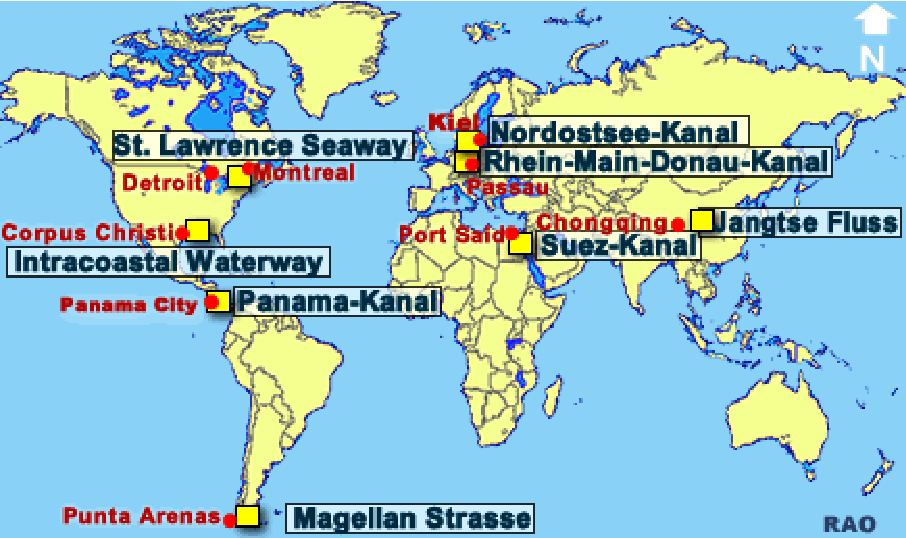
\includegraphics[width=.65\textwidth]{images/kanal}
\begin{citemize}
\item Suez-Kanal
\item Nord-Ostseekanal (Land nur 1m über Wasser $ \rightarrow $ Überflutungsgefahr und Geschwindigkeitsbegrenzung von 1.5km/h; Bau vor dem ersten Weltkrieg, Erleichterung des Handels, Umfahren von Dänemark)
\item Kanalsystem Frankreich
\end{citemize}
\paragraph{Panamakanal}
1881 begann eine französische Gesellschaft unter der Leitung von de Lesseps mit dem Graben des Kanals. 1898 wurden die Arbeiten eingestellt, da:
\begin{citemize}
\item ganzes Kapital aufgebraucht (262 Mio. \$)
\item 22000 durch Gelbfieber und Malaria getötete Arbeiter
\item keine Mittel gegen die natürlichen Gefahren in Panama
\item finanzielles Missmanagement, Bestechung, Falschinformationen
\item nur 25\% der Bauten fertiggestellt
\end{citemize}
1898 begannen sich die USA für Mittelamerika zu interessieren (Kuba $ \rightarrow $Befreiung von Spanien). USA bieten Kolumbien einen Kanalvertrag an (10 Mio. \$ plus jährlich 250’000 \$). Nach der Ablehnung durch Kolumbien unterstützen die USA die Unabhängigkeitsbewegung in Panama, das sich darauf von Kolumbien lösen kann. Vertrag 1903 mit Panama (10 Mio. \$, jährlich 250’000 \$ plus Abtretung eines 16km breiten Kanalstreifens). Die Amerikaner vernichten zuerst durch Drainage die Malaria und das Gelbfieber. Aufbau der Infrastruktur für die Arbeiten vor dem Eintreffen der Arbeiter $ \rightarrow $ Bau einer Eisenbahn. Entscheid keinen Kanal auf Meereshöhe zu bauen, sondern je drei Schleusen zwischen dem Gatunsee und den Meeren zu bauen. Im August 1914 konnten die USA den Kanal, früher als geplant, der 352 Mio. \$ gekostet hatte, eröffnen. Die Kanalzone war bis 1999 US-amerikanisches Hoheitsgebiet. Es passieren über 15’000 Schiffe den Kanal und können somit zwischen 5000 und 8000 Km Fahrt ersparen.
\subsection{Lufttransport am Beispiel: Berliner  Luftbrücke}
\subsubsection{Vorgeschichte}
März 1948 führten die West-Alliierten in den drei westlichen Zonen und in den drei westlichen Sektoren Berlins eine neue Währung ein. Die Sowjetunion wollte diese Währungsreform verhindern und benützte diese um die West-Alliierten unter Druck zu setzen und sie aus West-Berlin rauszuwerfen. Daher waren am 25. Juni alle Strassen- und Eisenbahnlinien zwischen den Westzonen und West- Berlin \glqq defekt\grqq und konnten nicht befahren werden $ \rightarrow $ Blockade von West-Berlin.  Die Amerikaner mussten nun entscheiden, ob sie West-Berlin fallen lassen oder ob sie einen Konflikt mit der Sowjetunion riskieren wollten. Welche Möglichkeiten boten sich den USA? \\
\begin{citemize}
\item Rückzug aus Berlin und Deutschland (Beginn Rückzug aus Europa)
\item Atom-Drohung gegenüber der SU aussprechen (USA hatten A-Bomben Monopol)
\item Nachschub nach West-Berlin freikämpfen (Krieg mit der Sowjetunion)
\item Luftbrücke
\end{citemize}
\subsubsection{Luftkorridor war nicht gesperrt aber:}
\begin{citemize}
\item Keine Transportflugzeuge
\item Keine Piloten (aber demobilisierte \glqq kennen \grqq den Weg nach Berlin)
\item Beschränkte technische Möglichkeiten
\item Ungewissheit über die Reaktion der Sowjetunion
\item Risiko von Abschuss durch SU (Sicher: in Flugbahn / Korridor bleiben – 5km breit)
\end{citemize}
\subsubsection{Notwendigkeit einer Lösung}
Täglich 3475 t Lebensmittel, Kohle, Rohstoffe, Treibstoff, usw. An Flugzeugen standen die Douglas C-47 zur Verfügung (3t Transportkapazität). Später konnten Douglas C54-Skymaster (10t Transportkapazität) eingesetzte werden. Die Amerikaner entwickelten ein kombiniertes Schiff-, Landverkehr- und Luftverkehrssystem (Container). Der nördliche- und südliche Luftkorridor wurde für den Hinflug, der mittlere Korridor für den Rückflug reserviert. Verschiedene Flughöhen für USA und UK wurden eingeführt. Es wurde ein dritter Flughafen in West-Berlin gebaut (Tegel). Jedes Flugzeug durfte nur einmal den Flughafen anfliegen (Nur ein Landeversuch, sonst zurück und erneut über Korridor anfliegen). Standardisierte Flugrouten und Flugverhalten. Anfänglich konnte alle 3min, später alle 90sek ein Flugzeug landen, 30min später wieder zurückfliegen. Die sowjetischen Störmanöver führten zu Abstürzen und dem Tod von 73 Piloten. Durch Dehydrierung der Lebensmittel konnte Gewicht und Volumen gespart werden.  Im April 1949 konnten an einem Tag durch 1383 Flüge 12’941 t Güter nach West-Berlin geflogen werden. Erfindung und Einsatz des GCA-Anflugsystems (Ground Control Approach). Die Sowjetunion beendete die Blockade am 12. Mai 1949. Mit 277’569 Flügen waren 2.3 Mio. t Fracht nach und 81’730 t Fracht aus West-Berlin geflogen worden.  Die Luftbrücke hatte die USA 233 Mio. \$ gekostet. Die erste \glqq Schlacht\grqq im Kalten Krieg hatte die Sowjetunion verloren. Gewaltige technische Fortschritte in der Luftfahrt.
\subsection{Vergleich See- / Landtransport vor dem 19. Jahrhundert}
\begin{tabularx}{1\textwidth}{L{2cm} L{5cm}  X}
\rowcolor[gray]{.6} \textbf{-} & \textbf{Seetransport} & \textbf{Landtransport} \\ 
Vorteile &  Tiefe Betriebskosten \newline Ferntransport (Luxusgüter, bei denen Preis entscheidende Rolle spielte) & Keine natürlichen Gefahren \\
\rowcolor[gray]{.9} Nachteile& hohe Investitionskosten \newline Gefahr eines Gesamtverlustes (Versicherungskosten) \newline Gefahr der Piraten & hohe Personalkosten \newline Gefahr Strassenraub\\
\end{tabularx}
\section{Lebensmittel}
Immer die spezielle Situation der Schweiz berücksichtigt – einem Land, das seit Jahrhunderten auf den Import von Lebensmitteln angewiesen ist. Bekannteste Schweizer Spezialitäten: Birchermüesli, Schokolade, Fondue.
\subsection{Wie produzieren wir die Lebensmittel?}
Vor der Neolithischen Revolution: keine Produktion. Mit der Neolithischen Revolution: Übergang zur Produktion von Lebensmitteln. Bewässerungssysteme als staatliche Grundlage in Ägypten und im Zweistromland. Plantagenwirtschaft mit einer hochentwickelten Agrarwirtschaft zur Römischen Zeit. Niedergang der Landwirtschaft im Frühen Mittelalter. Nach der Entdeckung Amerikas vergrössert sich die Anzahl der produzierten Lebensmittel (Tomaten, Kartoffeln, usw.). Verbesserungen in der Landwirtschaft während dem Mittelalter durch die Einführung der Dreifelderwirtschaft (links) und Fruchtfolgewirtschaft(rechts):\\
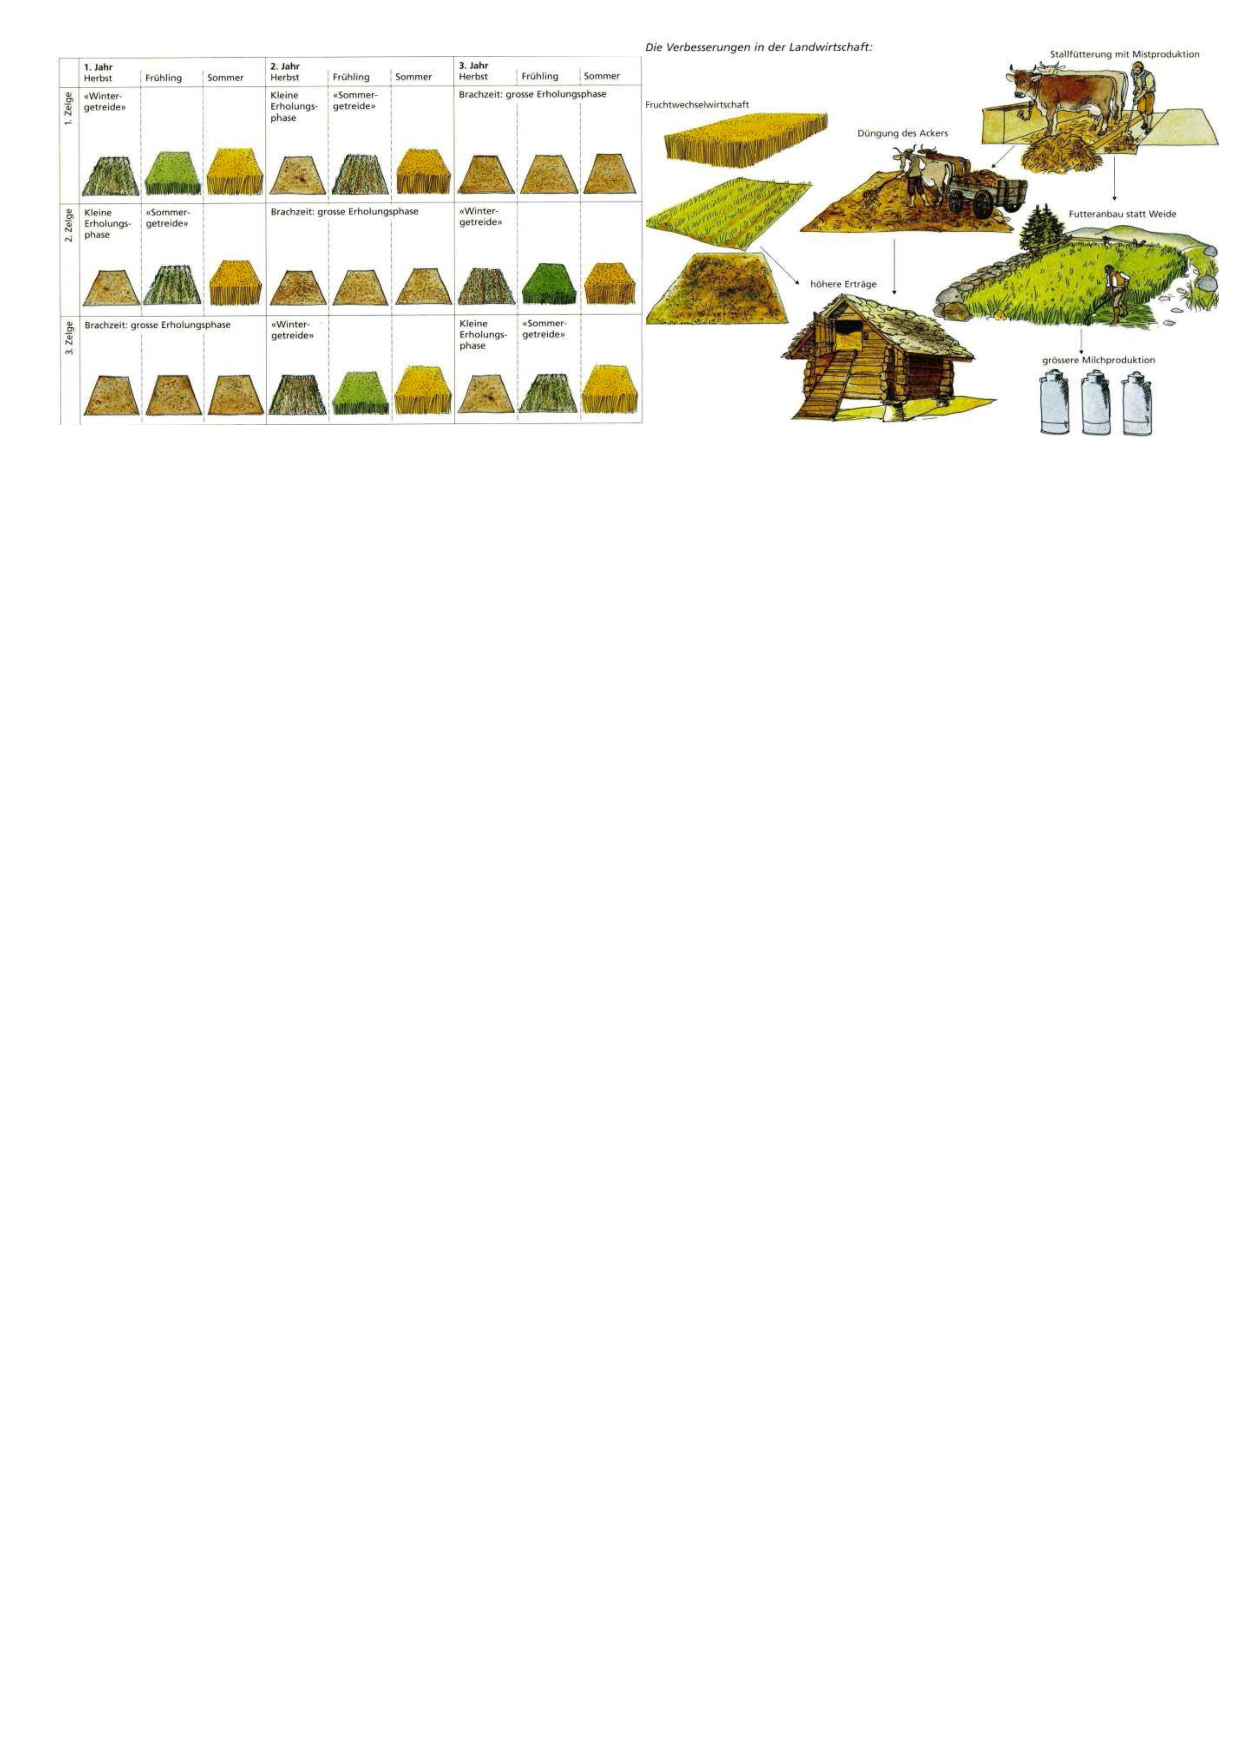
\includegraphics[width=1\textwidth]{images/felderwirtschaft}
\subsubsection{Weitere Produktivitätserhöhung dank Erfindungen und Entdeckungen während der Aufklärung und der Industrialisierung}
Neben dem natürlichen Dünger den Kunstdünger. Zucht von Tieren und Pflanzen. Neue Methoden der Haltbarkeit (Bsp. Pasteurisieren). Neue Verarbeitungsmethoden führen zu neuen Produkten. Verbesserte Transportmittel führen zu einem grösseren Exportradius.
\subsection{Wie veredeln wir die Lebensmittel?}
\textbf{Philipp Suchard (1797 - 1884)}\\
Kommt als Nachkomme hugenottischer Flüchtlinge in Neuenburg auf die Welt. Kauf in der Drogerie Matthieu Schokolade als Medizin – sieht eine Geschäftsmöglichkeit. Ausbildung als Zuckerbäcker und Reise nach Amerika. 1826 Beginn der industriellen Schokoladenproduktion uns später Kontakt mit Cailler. Ausweitung seiner beruflichen Tätigkeit auf die Schifffahrt und die Seidenraupen-Zucht. Setzt neue Aspekte in der Werbung. Suchard vergrösserte sich durch den Auf- und Zukauf anderer Lebensmittelproduzenten und lancierte
neue Produkte – 1982 Aufkauf durch Kraft Food – 1995 Einstellung der Schokoladenproduktion.
\subsection{Wie verteilen wir die Lebensmittel?}
\textbf{Gottlieb Duttweiler (1888-1962)}\\
Bei tiefen Preisen setzt man grosse Mengen ab – und macht Profit. Stetige Ablehnung von Verkauf von Tabak und Alkohol. In der Zürcher Altstadt geboren, \glqq KV\grqq, Erfolglos als Bauer in Brasilien. 1925 Gründung der Migros und erste fahrende Läden. 1928 erste eigene Produktionsstätte. 1935 Gründung von Hotelplan und der Zeitung \glqq Tat\grqq und Einstieg in die Politik (NR/SR bis 1962). Kandidatur in 5 Kantonen (überall gewählt) $ \rightarrow $ neues Gesetz: nur in 1 Kanton antreten möglich. 1940 Umwandlung Migros in eine Genossenschaft. 1944 Gründung der Migros-Klubschule. 1948 erster Selbstbedienungsladen. 
\subsubsection{Beeinflussung unseres Lebens durch die Migros}
Alle Schweizer konsumieren die gleichen Produkte. Durch die dominierende Marktstellung kann die Migros grosse Teile der Wirtschaft beeinflussen. Das ganze Konsumleben wird von einer Firma bezogen. Neue gesellschaftliche und wirtschaftliche Entwicklungen können von der Migros angestossen werden. Migros ist zu einem der Identifikationspunkte der Schweizer geworden.
\subsection{Wie konsumieren wir die Lebensmittel?}
\textbf{Else Züblin Spiller (1881 - 1948}\\
Unglückliche Jugendjahre. Erste journalistische Erfahrungen und Organisatorin von Kinderhilfstagen. 1914 Eröffnung von 19 Soldatenstuben beim Ausbruch des Ersten Weltkrieges. Unterstützung der Armee: Entlastung der Armee, Leute unter Kontrolle, kleine Ausgaben. 1918 erste Arbeiterkantine in der Maschinenfabrik Bühler in Uzwil. 1920 Umbenennung von \glqq Schweizer Verband Soldatenwohl\grqq in \glqq Schweizer Verband Volksdienst\grqq (SV). Konzept aus der Soldatenstube aus dem ersten Weltkrieg in die Industrie übernommen mit den Vorteilen: Essen von Familienmitglieder / Gewerkschaften nicht an Fabrik gebracht $ \rightarrow $ keine schlechten Einflüsse auf die Arbeiter. 1928 erstes Restaurant mit Selbstbedienung (mit Skepsis der Bevölkerung). Hausarbeit reduzieren $ \rightarrow $ Frau fordert Gleichberechtigung.
\subsubsection{Beeinflussung durch Else Züblin-Spiller}
Kürzere Mittagspausen – es wird nicht mehr zu Hause das Mittagessen eingenommen (Schule / Fabrik). Angleichung der Bevölkerungsschichten (gleiches Essen / Kantine). Veränderung bei den Essgewohnheiten können beeinflusst werden (gesundes Essen). Der Anteil der Ausgaben für die Ernährung vermindert sich (günstig). Normale Gaststätte müssen sich umorientieren. Die Vorbereitung der Speisen führt zu neuen Berufsfeldern. 
\subsection{Zukunft der Lebensmittelindustrie}
Online Bestellung; Lieferung nach Hause; Höhere Produktion; Gentechnik (Gentechnisch veränderte Reispflanzen (Produktion Provitamin A) $ \rightarrow $ niemand will den Golden Rice)
\section{Energie – von Muskelkraft zu Atomenergie}
\subsection{Historischer Abriss der Energienutzung durch den Menschen}
\subsubsection{Erste und bis heute wichtigste Energiequelle ist die Nahrung}
Anfänglich waren dies Pflanzenteile, Samenkörner, Früchte, Nüsse und Wurzeln. Das Sammeln, speziell von Nüssen, erbrachte einen Energiegewinn (bis zu 15 Mal grösser Ertrag im Verhältnis zum Aufwand). Fleisch durch die Jagd zu bekommen lohnte sich nur bei grossen Pflanzenfressern, die fettreiches Fleisch besassen. Durch die Erfindung des Speeres vor rund 400'000 Jahren konnte ein höherer Energiegewinn erreicht werden. Fischerei lohnt sich vor allem dort, wo grosse Fischschwärme der Küste entlang schwammen. Je nach Nahrungsangebot konnte eine unterschiedliche Bevölkerungsdichte erreicht werden: Fischereigebiete bis zu 100 Menschen/km\textsuperscript{2} ; Wald und Jagdgebiet bis zu 10 Menschen/km\textsuperscript{2} ; Steppenregionen rund 1 Mensch/km\textsuperscript{2}. 
\subsubsection{Zweite Energiequelle des Menschen: Das Feuer}
Vor rund 1 Mio. Jahre lernte der Mensch das Feuer zu beherrschen. Einige Historiker betrachten dies als den wichtigsten Schritt zum Menschsein. Die Auswirkungen der Verwendung des Feuers sind Licht, Wärme, Schutz, Vorratsgefässe aus Ton brennen, Jagen, einfache Wald-Rodung, Metalle einschmelzen / formen, Garen von Lebensmittel (diese werden effizienter), Durch braten / kochen wird enzymatischer Aufschluss.
\subsubsection{Der Mensch braucht Wärme und Licht}
Zum Kochen, erwärmen der Häuser und der Herstellung von Ziegeln wurde ursprünglich nur Biomasse eingesetzt. Wichtigster Brennstoff war dabei das Holz. Herstellung von Glas. Das immer grösser werdende Schmelzen von Eisen (1t Eisen verbraucht 1’000t Holz) führte ab dem 13. Jahrhundert in Europa zu einem Holzmangel. Der Holzmangel führte zur Verwendung der unbeliebten Kohle. Zur Beleuchtung verbrannte der Mensch in Tonlampen tierische und pflanzliche Fette (zb Walfett).
\subsection{Beginn der Landwirtschaft}
Neben der menschlichen stehen nun auch tierische Muskeln zur Verfügung. Für den Transport von Gütern wurden Ochsen, Pferde, Kamele und Yaks eingesetzt. Gewisse Tiere (bspw. Pferd) stehen jedoch in der Konkurrenz zum Menschen was die pflanzliche Nahrung betrifft. Kühe und Ochsen werden daher bevorzugt, da sie als Wiederkäuer auch Zellulose nutzen konnten, also auf minderwertigem Weideland ihr Futter fanden. Das Pferd wurde erst ab dem 12. Jahrhundert als Zugtier eingesetzt. Es brauchte eine grössere Futterfläche und das Kummet musste verbreitet sein. Daneben erbrachten immer noch Sklaven und Leibeigene (Abgabe an Grundeigentümer) die hauptsächliche Arbeitsleistung. 
\subsection{Energieformen}
\subsubsection{Wasser- und Windmühlen}
Mit den Wasser- und Windmühlen kam die erste mechanische Energieumwandlung auf. Mit Mühlen wurden Getreide gemahlen, Öle gepresst, Metall bearbeitet. In Europa ab dem 10. Jahrhundert verbreitet. Erlebt im Rahmen der Energiewende wieder eine Renaissance.
\subsubsection{Kohle}
In der vorindustriellen Zeit wurde nur ungern die dreckige Kohle verwendet. Die Vorteile der Kohle waren und sind Hohe Energiedichte, transportier- und lagerbar, standortunabhängige Verwendung, Je nach Verwendungszweck unterschiedliche Kohle einsetzbar. Ab 1882 wurde Kohle zur Stromerzeugung eingesetzt. Der Einsatz von Kohle hatte und hat eine massive Luftverschmutzung zur Folge. Diese Luftverschmutzung war während den Industriellen Revolution in Europa von Bedeutung und ist es heute in vielen Schwellenländern.
\subsubsection{Strom}
Vorteile von Strom gegenüber der Kohle: Jederzeit und sofort verfügbar, Keine Umweltschäden beim Konsumenten, Keine schmutzigen Hände beim Verbrauch, Als erneuerbare Energie einsetzbar. Heute werden weltweit zwei Drittel der
Stromproduktion durch Kohle, Gas und Öl erzeugt. Das dritte Drittel wird je hälftig von Wasserkraft und Atomkraftwerken erzeugt. Stromherstellung durch: Wasserkraft (Speicherkraftwerke, Laufkraftwerke, Pumpspeicherkraftwerke), Atomkraftwerke, (Braun-) Kohle Kraftwerke, Erdgas-Kraftwerke, Biomasse-Kraftwerke, Geothermische Kraftwerke, Photovoltaik-Anlagen (Sonnenkollektoren), Windkraftwerke, Müllverbrennungsanlagen.\\
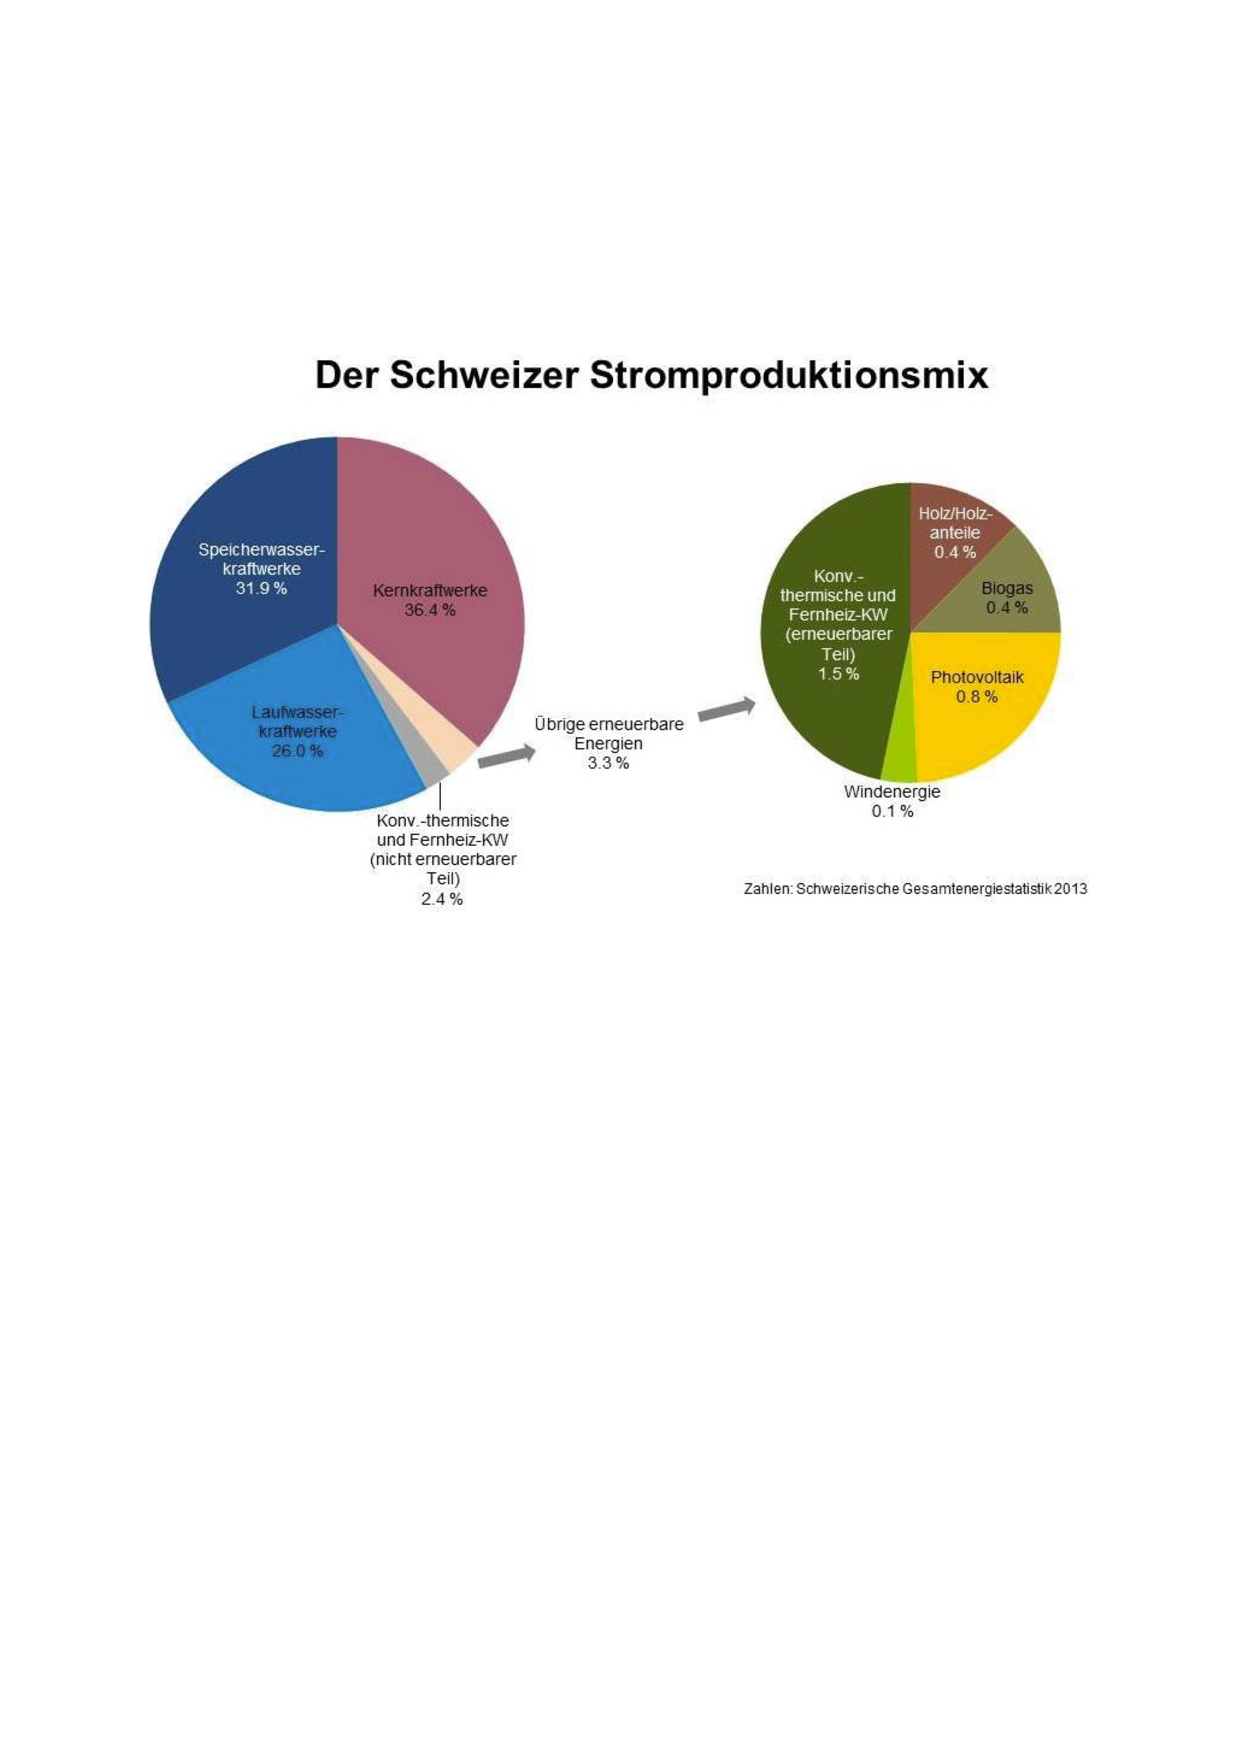
\includegraphics[width=.8\textwidth]{images/strommix}

\subsubsection{Erdöl}
Wurde zum Abdichten der Boote, zur Beleuchtung und als Medizin zur Wundbehandlung verwendet. Um das immer teuer werdende Walöl zu ersetzen, schlägt ein New Yorker, Petroleum als Beleuchtungsmittel einzusetzen. Die darauf erfolgte Suche nach Erdöl führt 1859 zum Fund in Titusville (Pennsylvania) einem ergiebigen Erdölfeld. Durch den 1865 beendeten Bürgerkrieg, der in Schwung kommenden Industrialisierung, der Erschliessung des Westens, der starken Einwanderungswelle aus Europa und dem riesigen Binnenmarkt, herrschten euphorische Zuversicht. John D. Rockefeller sieht in dieser Situation die Perspektiven für das Öl: Gründung 1870 der Standard Oil Company, Diese übernimmt den gesamten Produktionsvorgang, Wird erstes multinationales Unternehmen. Die aufkommende Krise wegen den elektrischen Glühbirnen von Edison wird durch die Produktion von Ölöfen und dem 1886 erfundenen Verbrennungsmotor von Benz gelöst. 1871 wird am Kaspischen Meer Öl gefunden. 1901 wird ein riesiges Ölfeld in Texas gefunden (Gründung: Texaco). 1907 wird im niederländischen Ost-Indien (heutiges Indonesien) Öl gefunden (Gründung Royal Dutch / Shell Group). 1908 wird in Persien Öl gefunden (Gründung Persian Oil Company, heute BP). 1911 der Oberste Gerichtshof der USA zerschlägt Standard Oil. 1911 der englische Marineminister Churchill entscheidet die Flotte auf Ölfeuerung umzustellen. 1912 gab es in den USA 900’000 Autos (1900 erst 9000). 1913 wird das cracken patentiert – grössere Ausbeute von Benzin. Im Ersten Weltkrieg werden erstmals Motorfahrzeuge eingesetzt. In den 1920er Jahren wurde Erdöl im Irak, in Mexiko und in Venezuela gefunden. In den 1930er Jahren wurden auf der Arabischen Halbinsel die grössten Erdölfelder entdeckt und von den Amerikanern und Engländern durch Verträge abgesichert. In der Zwischenkriegszeit ging man über statt das Benzin in den Läden zu kaufen nun Tankstellen zu errichten. 1930 kostete 1 Barrel Öl 10 Cents. Während dem Zweiten Weltkrieg gelang es den Deutschen nicht im genügenden Ausmass synthetischen Treibstoff aus Kohle herzustellen. In den 1950er Jahren stritten Standortstaaten und Ölgesellschaften über den Besitz des Öls. Die goldene Zeit des Erdöls während den 1960er Jahren endete mit der ersten Ölkrise ab 1973 (Ölboykott westlicher – pro israelischer Staaten) Wirtschaftseinbruch. 1979/1980 Zweite Ölkrise wegen dem Iran-Irak Krieg. Einige Länder versuchen durch eigene Ölförderung, durch die Nutzung anderer Energieträger oder durch Sparmassnahmen die Abhängigkeit vom Öl zu vermindern.
\subsubsection{Erdgas}
Bereits 1883 erste städtische Beleuchtungen mit Erdgas. Durch das Aufkommen der Elektrizität ging die Nachfrage nach Erdgas zurück. Durch die Entwicklung der Hochdruck-Pipelines wird Erdgas wieder attraktiv. Ab den 1980er Jahren spielt Erdgas eine immer grössere Rolle (Stromerzeugung, In der Industrie, Zur Raumheizung, Zur Herstellung von Kunstdünger). Heute rund 25\% des weltweiten Energiebedarfs durch Erdgas abgedeckt.
\subsubsection{Energieverbrauch der Welt}\vspace{-1.5cm}
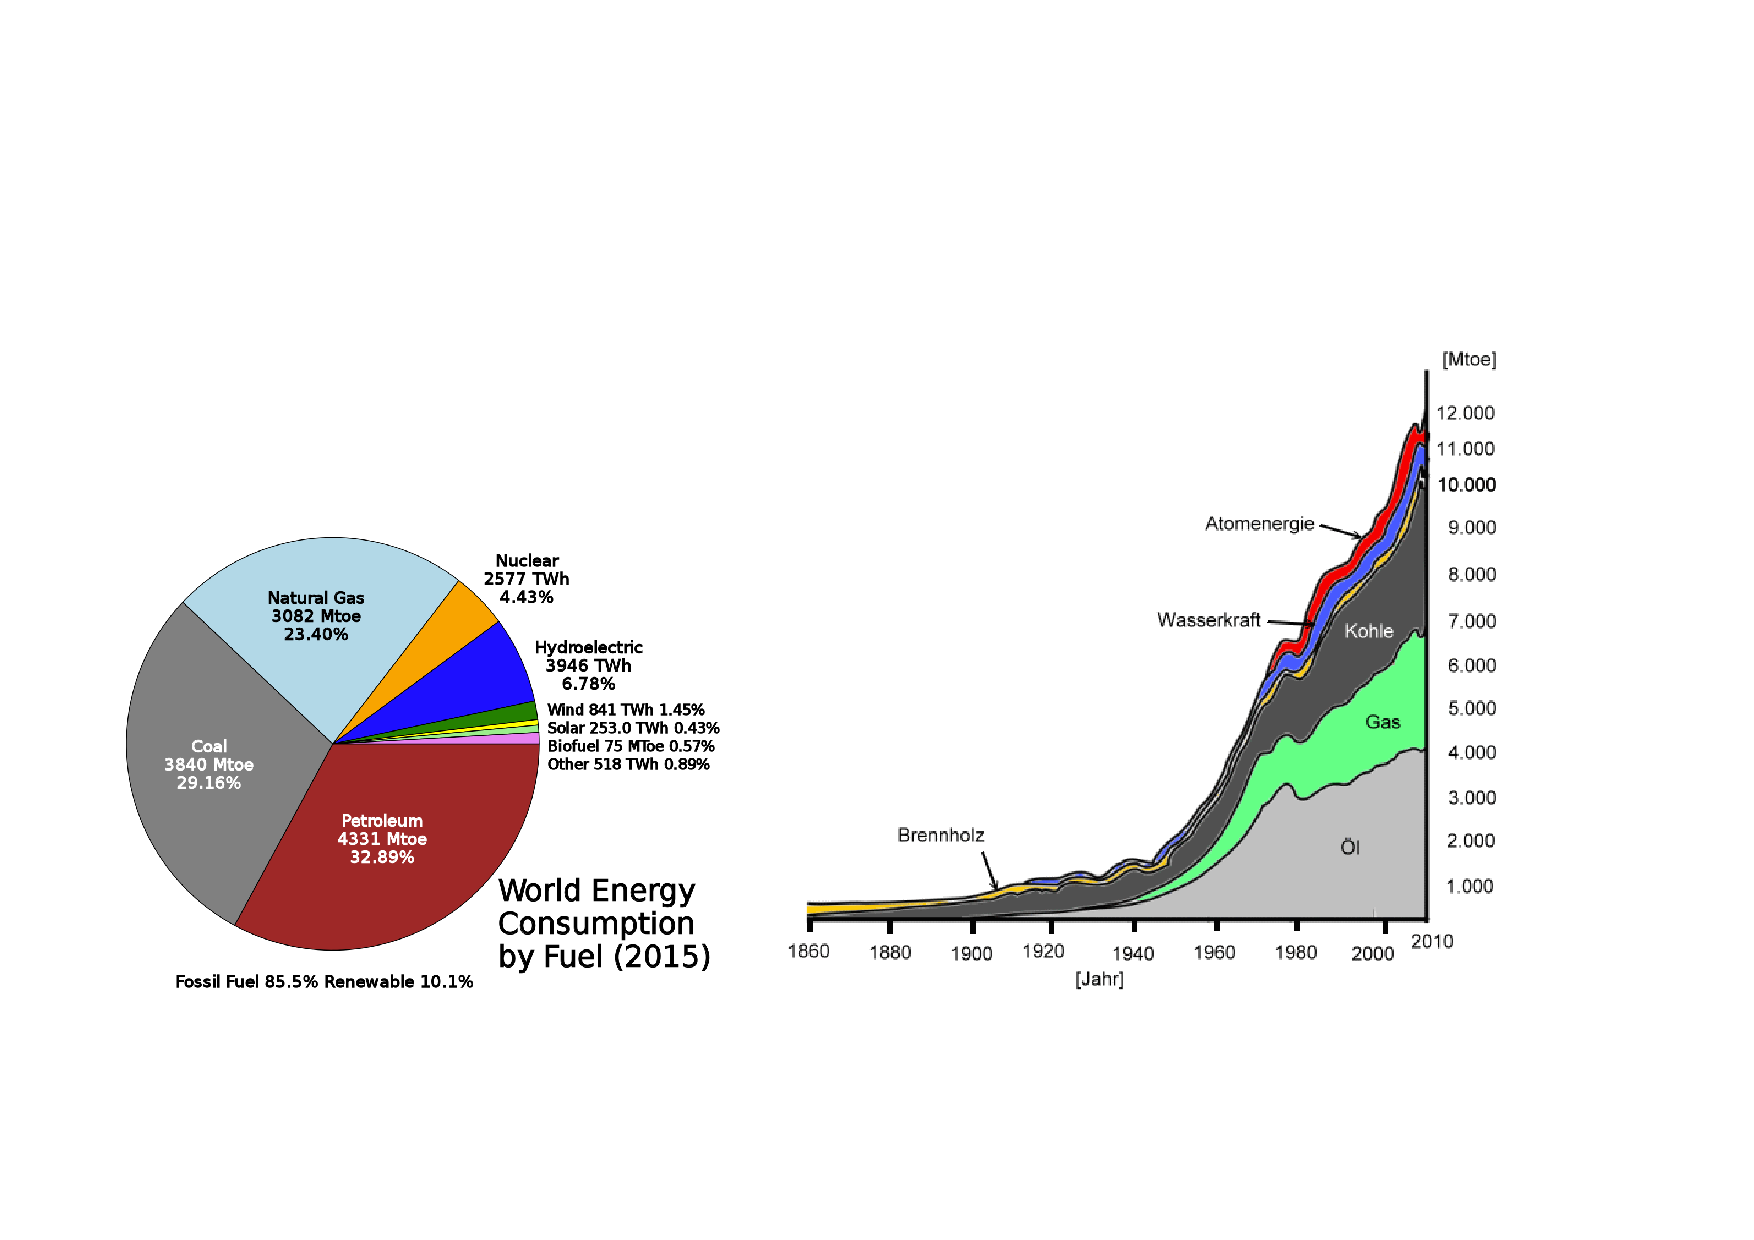
\includegraphics[width=.8\textwidth]{images/energiewelt} \vspace{-.5cm}
\subsubsection{Energieverbrauch der Schweiz}
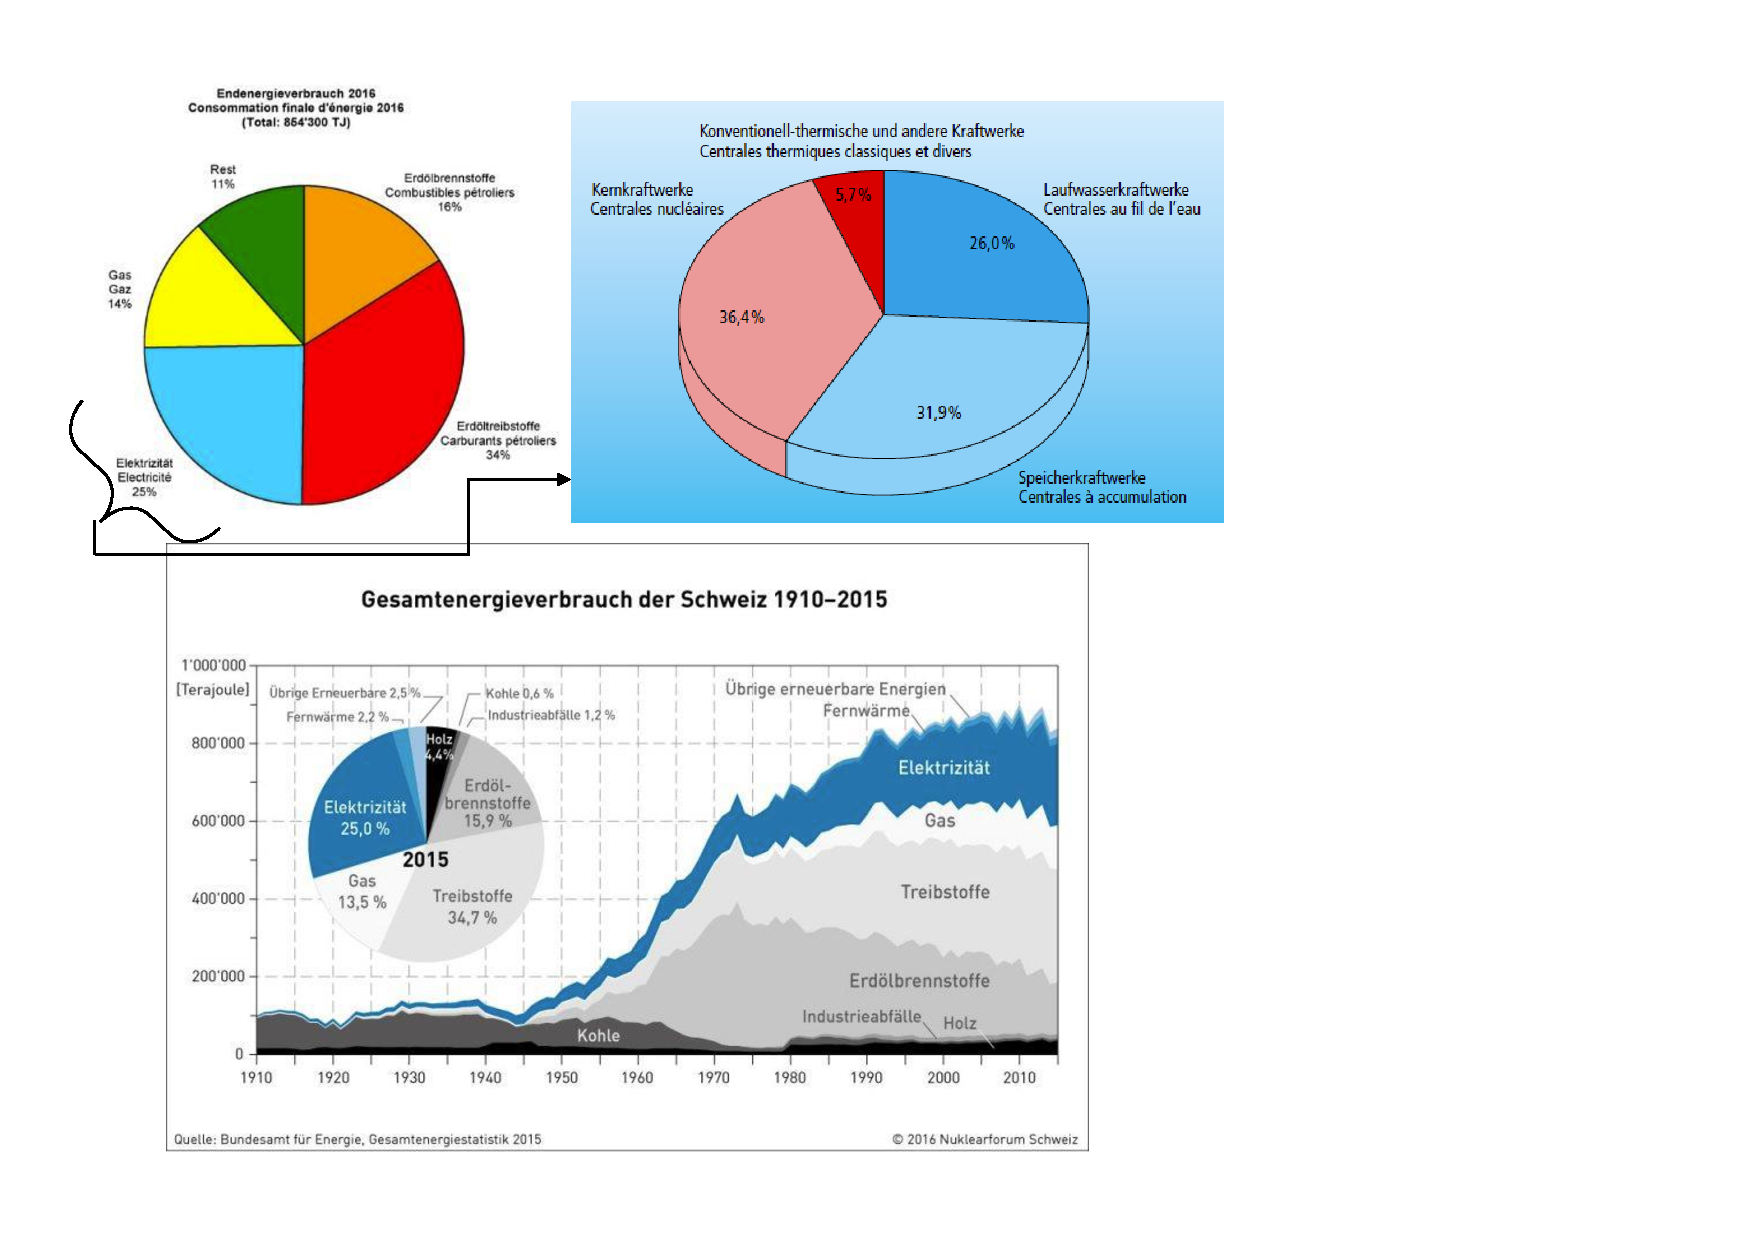
\includegraphics[width=.9\textwidth]{images/energieschweiz} \\
Ein Schweizer verbraucht rund 130kWh/Tag, was der Arbeit von über 75 Menschen entspricht. Für rund die Hälfte der Menschheit sind aber immer noch Muskelkraft, Haustiere, Holz, Dung und pflanzliche Reste hauptsächlichen Energiequellen.
\section{Kommunikation}
\subsection{Warum kommunizieren wir?}
Wir wollen dem Mitmenschen etwas über uns mitteilen (Sachinformation und Beziehung). Menschliche Beziehungen basieren auf Kommunikation – Nicht-Kommunikation ist auch Kommunikation.
\subsection{Wie kommunizieren wir?}
Informationen müssen zuerst \textbf{kodiert} werden. Informationen werden dann \textbf{übermittelt}. Informationen werden \textbf{dekodiert}. Informationen werden \textbf{gespeichert}.
\subsection{Historischer Ablauf der Kommunikationsentwicklung}
\begin{citemize}
\item 20’000 v. Chr. Felszeichnungen
\item 4000 v. Chr. Erste Schriftzeichen
\item 1450 Erfindung Buchdruck
\item Testbetrieb Morsetelegraph
\item 1876 Erfindung Telefon
\item 1920 erste Rundfunkstation
\item 1987 erstes tragbares Funktelefon
\item 1990 Privatpersonen können das Internet verwenden
\end{citemize}
\subsubsection{Berühmte mündliche Kommunikation}
Der Meldeläufer von Marathon 490 v. Chr.. Heureka ist altgriechisch ($\varepsilon\upsilon\rho\eta\kappa\alpha$) und heisst \glqq Ich habs\grqq . Der Spruch ist vor allem im Zusammenhang mit Archimedes von Syrakus berühmt geworden. Dialektische Gesprächskultur bei den alten Griechen. Gespräche mit Gott/Göttern – Gebete. Freimaurische Gesprächskultur. Reden: \glqq Ich bin ein Berliner!\grqq; \glqq no surrender!\grqq ; \glqq Wer zu spät kommt, den bestraft die Geschichte\grqq .
\subsubsection{Verbale/non verbale Sprache zur Kommunikation}
Vorteile:\\
spontanes Nachfragen möglich (Präzise \& unpräzise Aussagen), viele Sinne sind an der Kommunikationsvermittlung beteiligt, keine Kosten, Mensch ist ein soziales Wesen – braucht mündliche Kommunikation\\ Nachteile:\\
Missverständnisse möglich – Kodierung muss klar sei, Nur direkt möglich – keine Gespräche auf Distanz ohne technische Hilfsmittel, Nur beschränkte Informationsvermittlung möglich\\
Was kommunizieren wir mündlich?\\
Persönliches, Unbedeutendes, Schnelllebendiges\\
Auf was ist bei der verbalen/non verbalen Kommunikation zu achten?\\
Mimik kann missverstanden werden, klare Definitionen müssen vorhanden sein
\subsubsection{Kommunikation mit Bildern}
Vorteile:\\
Mensch glaubt eher was er sieht, schwierige Zusammenhänge/Informationen können besser dargestellt werden, einfaches Lernen und memorisieren möglich, grössere emotionale Reaktionen möglich\\ Nachteile:\\
Bilder sind immer nur Momentaufnahmen, Fälschungen?, Bearbeitung? mit einer tendenziösen Intension
\subsubsection{Übergang von den Bildern auf die Schriftzeichen}
Ideogramme, Piktogramme – Phonetisierung der Zeichen (Keilschrift und Hieroglyphen):\\
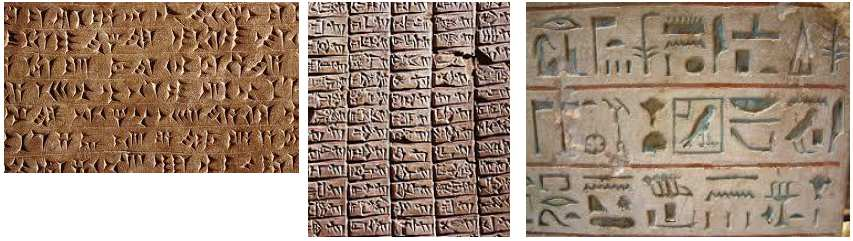
\includegraphics[width=.8\textwidth]{images/hyro}
\subsection{Wieso verwendet der Mensch die Schrift/Schriftzeichen?}
Besitzverhältnisse und Rechtsverhältnisse festlegen und für die Zeit sichern. Schneller Fixierung. Machtausübung leichter möglich. An Lautzeichen braucht es weniger Zeichen als an Piktogrammen. Wissen und Traditionen können für die Nachwelt erhalten bleiben.
\subsection{Was sind die Auswirkungen der Verwendung der Schrift?}
Es entsteht eine neue Klasse von Mächtigen (die der Lese- und Schreibkundigen). Ausbildung ist notwendig um an das Wissen zu kommen. Der Staat kann seine Herrschaft direkter und zentraler ausüben. Standardisierung der Sprache ist notwendig. Ausdrucksmöglichkeiten sind eingeschränkt.
\subsection{Buchdruck}
Um 1450 Durchbruch des Buchdruckes. Auswirkungen des Buchdrucks: Massive Zunahme des Wissens, Wissen wird bezahlbar, transportierbar, breiter gestreut, Humanismus und Reformation, Zeitungen können nun erscheinen, Allgemeine Schulpflicht wird eingeführt, Standardisierung der Schrift.
\subsection{Telefon}
1837 erfindet Samuel Morse den Telegraphen – erste nutzbringende Anwendung der Umwandlung von Sprache in elektrische Impulse. Zahlreiche technische Entwicklungen von funktionierenden Telefonapparaten, die jedoch nie über den Labor-Versuch hinwegkamen. Das ab 1878 gebräuchliche Kohlemikrofon erlaubte eine vergrösserte Reichweite. 1891 erste automatische Selbstwahl. Ab 1926 Mobiltelefone in der Deutschen Reichsbahn. 1955 Mehrfrequenzwahlverfahren durch Bell Telefone. Vorteile: Schneller und relativ billiger Informationsaustausch, Öffentlich, aber trotzdem privat. Nachteile: Nur noch die Sprache als Übermittler – keine Mimik und Gestik, Weniger Freizeit – jederzeit erreichbar, Schnelllebendigere Zeit.
\subsection{Internet}
1957 Sputnik erster Satellit. Ab den 1960er Jahren Idee einer Paketvermittlung und eines Netzwerkes. 1969 erste Verbindung zwischen Grossrechnern und dem Austausch von Botschaften (29.10.1969). 1972 Entwicklung des ersten E-Mail-Programms. 1974 erste Erwähnung des Bergriffs Internet. 1985 erste Domain. 1990 Freigabe des Internets für kommerzielle Nutzung (privater Gebrauch). 1993 Freigabe von WWW. 2001 Wikipedia wird gegründet. \vspace{-0.2cm}
\subsubsection{Auswirkungen des Internets}
\begin{citemize}
\item weltweite und billige Kommunikation möglich
\item Informationen und Wissen sind weltweit und günstig abrufbar
\item einheitliche Meinung in der Welt – Wikipedia weiss alles
\item statt persönliches Vereinsleben nun soziale Netzwerke
\item neue Formen der Politik, speziell durch soziale Bewegungen
\item neue Formen der Hilfe mit Peer-to-Peer-Kredite möglich
\item Neue Freizeitmöglichkeiten (YouTube)
\item Neue Vertriebsmöglichkeiten möglich
\item neue Möglichkeiten Informationen zu beschaffen
\item neue Sicht der Welt
\end{citemize}
\subsubsection{Vorteile}
\begin{citemize}
\item Schnelle Verfügbarkeit des nationalen und internationalen (Informations-)Angebots
\item Anonymität
\item Bequemlichkeit, Benutzerfreundlichkeit
\item Geschwindigkeit des Mediums
\item Aktualität (Aktualisierung von Informationen sehr rasch und einfach möglich)
\item Kostenersparnis
\item Zeitliche Unabhängigkeit (24 Stunden erreichbar)
\item Globale Kommunikation
\item Grosse Verbreitung
\item Möglichkeit des Informationsaustausches
\item Grafische Benutzeroberfläche
\end{citemize}
\subsubsection{Nachteile}
\begin{citemize}
\item Datenschutz, Sicherheitsproblematik
\item Kurzlebigkeit (z.B. von Informationen oder Webseiten)
\item Fruchtbarer Boden für illegale Geschäfte aufgrund mangelnder Rechtslage
\item Qualität der Informationen?
\item Spurenhinterlassen $ \rightarrow $Werbezusendungen, Sicherheit
\item Virenprogramme, Hacker...
\item Teilweise noch fehlende Akzeptanz des Mediums?
\item Voraussetzung für effektiven Gebrauch: Grundwissen über den Umgang mit dem Internet und Kenntnis effizienter Suchstrategien (ansonsten hoher Zeitaufwand und Frustrationserlebnisse, einfache Daten können nicht verstanden werden)
\item Technisches Grund – Know-how
\end{citemize}
\section{Messen – Rechnen}
\subsection{Messen}
Wieso messen wir? - Jede Aussage basiert auf ein Messen; Um zu vergleichen messen wir\\
Was messen wir? - Natürliche Phänomene wie Temperatur, Feuchtigkeit, Distanz, Gewicht, usw. ; Leistungen wie Geschwindigkeit und Kraft; Den Wert eines Gutes oder einer Dienstleistung mit der virtuellen Grösse Geld\\
Seit wann messen wir was? - Bevor wir messen können, brauchen wir die dazu notwendigen Messinstrumente und Masseinheiten
\subsection{Geld}
Wieso gibt es Geld? \\
Wir können einfacher zahlen, tauschen, vergleichen und aufbewahren (Geld regiert die Welt? ; Geld ist die Lebenskraft des Krieges? (Cicero); Geld verdirbt den Charakter?)\\
Was wurde bis jetzt als Geld verwendet?\\
Nützliche Gegenstände, die transportierbar, teilbar, abzählbar, in einer bestimmten Menge vorhanden und beständig waren. (Muscheln, Pfeilspitzen, Salz, usw.)(\textbf{Warengeld})\\
Metallklumpen führen zu Münzen (Metallwert entspricht Münzwert). Quittungen führen zu Banknoten. Bargeld führt zu Buchgeld und Plastikgeld. \\
Wieso akzeptieren wir bedrucktes Papier als Wert?\\
Vertrauen in die Politik der Nationalbank und der Geschäftsbanken. Vertrauen in die Qualität der Banknoten (Sicherheitsmerkmale). Keine anderen Möglichkeiten.
\subsubsection{Geschichte des Schweizer Franken}
Bis 1798 hatte jedes Gebiet in der Schweiz seine eigene Währung. 1798 führen die Franzosen den Schweizer Franken zu 10 Batzen und 100 Rappen ein. 1803 wurde der Schweizer Franken nur noch zu einer Berechnungsgrundlage für die wieder entstandenen kantonalen Währungen. 1850 wird der Schweizer Franken als Währung eingeführt. Dieser wird akzeptiert, jedoch spielt er anfänglich keine dominierende Rolle. Die Schweiz ist Teil der Lateinischen Münzunion und hat keine Notenbank, sondern 38 private und kantonale Notenbanken. 1907 Gründung der Nationalbank (SNB), die auch das Banknotenmonopol erhält. Während dem Ersten Weltweltkrieg Aufhebung des Goldstandards. Abwertung des Schweizer Frankens 1936 um rund einen Drittel. 1945 bis 1973 fixer Welchselkursim Rahmen des BrettonWoods Systems. Seit 1973 flexible Wechselkurse. 2011 bis 2015 Mindestkurs gegenüber dem Euro. Der Schweizer Franken wurde weltweit zu einem sicheren Hafen. Je nach Berechnungsart liegen bis zu einem Drittel des Weltvermögens auf Schweizer Banken. Der erwachsene Schweizer besitzt 2015 durchschnittlich 535’000 Franken. Die 1\% Reichsten besitzen 41\% des Gesamtvermögens in der Schweiz. 55\% besitzen weniger als 50’000 Franken. Seit 2016 neue (9.) Banknotenserie.
\subsection{Verwendete Masseinheiten}
Der Fuss ist eines der ältesten Längenmasse, die durchschnittliche Länge eines Männerfußes, ungefähr 30 cm. Die Elle im Zweistromland ein Kupferstab (\glqq Elle von Nippur\grqq) ca. 50 cm. Auch der Knochen zwischen Handgelenk und Ellbogen. Der Faden war in der Seefahrt als Längenmass für die Wassertiefe verwendet. Die Wegstunde, ist die Strecke, die ein Mensch in einer Stunde zurücklegt, ca. 5 Km. Die Seemeile (1,8 Km) und die Meile (1.6 Km) sind im anglo-amerikanischen Ländern. Seemeile in der
Seefahrt heute verwendet. Das Liter- und Meter-System war 1793 als erstes Dezimalsystem eingeführt und 1848 von der Schweiz übernommen. In der Alten Eidgenossenschaft hatte jeder Kanton seine eigene Währung in Form von Gulden, Batzen und Rappen (nicht dezimal). Zwischen 1798 und 1803 und seit 1848 gibt es den Schweizer Franken (seit 1924 auch im FL)
\subsection{Kalender}
\subsubsection{Kalendersysteme}
Mondkalender:\\
älteste Form von Kalender. Mondjahre sind kürzer als Sonnenjahre, da der Mondmonat 29,53 Tage dauert. Somit stimmt er mit den Jahreszeiten nicht überein. Der islamische Kalender ist ein Mondkalender.\\
Sonnenkalender:\\
basiert auf den Lauf der Erde um die Sonne (ca. 365.25 Tage). Somit stimmt er mit den Jahreszeiten überein. Sonnenkalender sind: gregorianische K., iranischer K., koptischer K. und Maya-Kalender.\\
Lunisolarkalender:\\
Berücksichtigt Sonnen-und Mond-Phasen. Gleicht mit Schalttagen deren unterschiedliche Länge aus. Beispiel: tibetischer K., jüdischer K. und alt-chinesischer Kalender.
\subsubsection{Jüdischer Kalender}
Gültigkeit:\\
In dieser Form seit 359 nChr. Seit dem 11. Jahrhundert in den jüdischen Gemeinden allgemein anerkannt.\\
Gliederung:\\
Jahre, Monate und Tage. Die Unterschiede von Sonnen-und Mondkalender werden innert 19 Jahren mit 7 30-tägigen Schaltmonat ausgeglichen.\\
Besonderheit:\\
Der Tag rechnet sich von Abend zu Abend. Die Welterschaffung wurde auf 3761 vChr. festgelegt.
\subsection{Der Julianische Kalender} 
Gültigkeit:\\
seit 45 vChr., eingeführt durch Julius Caesar. Teilweise ab 1582 vom Gregorianischen Kalender abgelöst, teilweise bis ins 20. Jahrhundert gültig, in den Ostkirchen bis heute. Silvesterkläusein Appenzell Ausserrhoden.\\
Gliederung:\\
Kalenderanfang am 1. März. Jahresdauer von 365.25 Tagen. Einzig bei Juli und August hat sich der Monatsname zu Ehren eines römischen Herrschers erhalten.\\
Besonderheit:\\
Bis 2099 beträgt der Unterschied zum Gregorianischen Kalender 13 Tagen.
\subsubsection{Der Gregorianische Kalender}
Gültigkeit:\\
Seit 1582 in katholischen Gebieten, seit 1701 in reformierten Gebieten (CH), seit 1812 im Kanton Graubünden.\\
Gliederung:\\
Jahreslänge von 365,2425 Tage. Alle 100 Jahre fällt das Schaltjahr aus.\\
Besonderheit:\\
Eingeführt durch Papst Gregor XIII. Nur eine Weiterentwicklung des Julianischen Kalenders.\\
Bedeutung:\\
Seit 1949 \glqq weltweit\grqq anerkannter Kalender
\paragraph{Bedeutung der Monatsnahmen}
\par
\begin{tabular}{l l}
Januar & Janus - Gott mit zwei Gesichtern\\
Februar & Göttin der Reinigung\\
März & Ehrung des Kriegsgottes Mars\\
April & Öffnung der Natur\\
Mai & Major, Natur vergrössert sich\\
Juni & Gott der die Ehe beschützt\\
Juli & Zu Ehren von Julius\\
August & Zu Ehren von Augustus, Sohn von Julius\\
September & Der Siebte Monat, Rechnung von März an (Frühlingsanfang)\\
Oktober & Der Achte Monat\\
November & Der Neunte Monat\\
Dezember & Der Zehnte Monat\\
\end{tabular}
\subsubsection{Islamischer Kalender}
Gültigkeit:\\
Seit 638 nChr., durch 2. Kalifen eingeführt. (0 = Hedschra)\\
Gliederung:\\
12 Mond Monate zu 29 oder 30 Tage. Jahresdauer 354 1/3 Tage. \\
Besonderheit:\\
Reiner Mondkalender. 33 Jahre islamischer Zeitrechnung entsprechen 32 Jahre christlicher Zeitrechnung. \\
Bedeutung: Für die islamischen Feiertage von Bedeutung. (Ramadan wechseln im Laufe der Jahre die Jahreszeiten).\\
\subsubsection{Weitere Moderne Kalender}
Positivisten Kalende:\\
1849 von Auguste Comte vorgeschlagen. 13 Monate à 28 Tage (+ 1 Totentag). Beginn: 1789 Französische Revolution. Monatsnamen nach Persönlichkeiten benannt. Alle religiösen Bezüge wurden gestrichen.\\
Faschistischer Kalender:\\
Marsch auf Rom und Machtübernahme der Faschisten 1922 als Beginn einer neuen Zeitrechnung angesehen. Auch die Nationalsozialisten führten einen neuen Kalender ein (Beginn: Hitler Putsch in München 1923)\\
Sowjetischer Revolutionskalender:\\
1929 bis 1940 im Gebrauch. 12 Monate zu je 6 Fünf-Tage Woche. 1931 dann auf Sechs-Tage Woche verändert.
\subsubsection{Masseinheiten der Zeit}
Woche: \\
7 Tage nach der Mondphase und/oder der Welterschaffung. Beginnt am Sonntag oder Montag.\\
Stunde:\\
Aufteilung des Tages in 24 Stunden seit dem Alten Ägypten. Heute über die Sekunde bei den Atomuhren definiert (3600).\\
Minute:\\
60stel einer Stunde (pars minuta= verminderter Teil) und in 60 Sekunden unterteilt. Es gibt auch die Industrieminute (1/100stel einer Stunde).
\subsubsection{Zeitzonen}
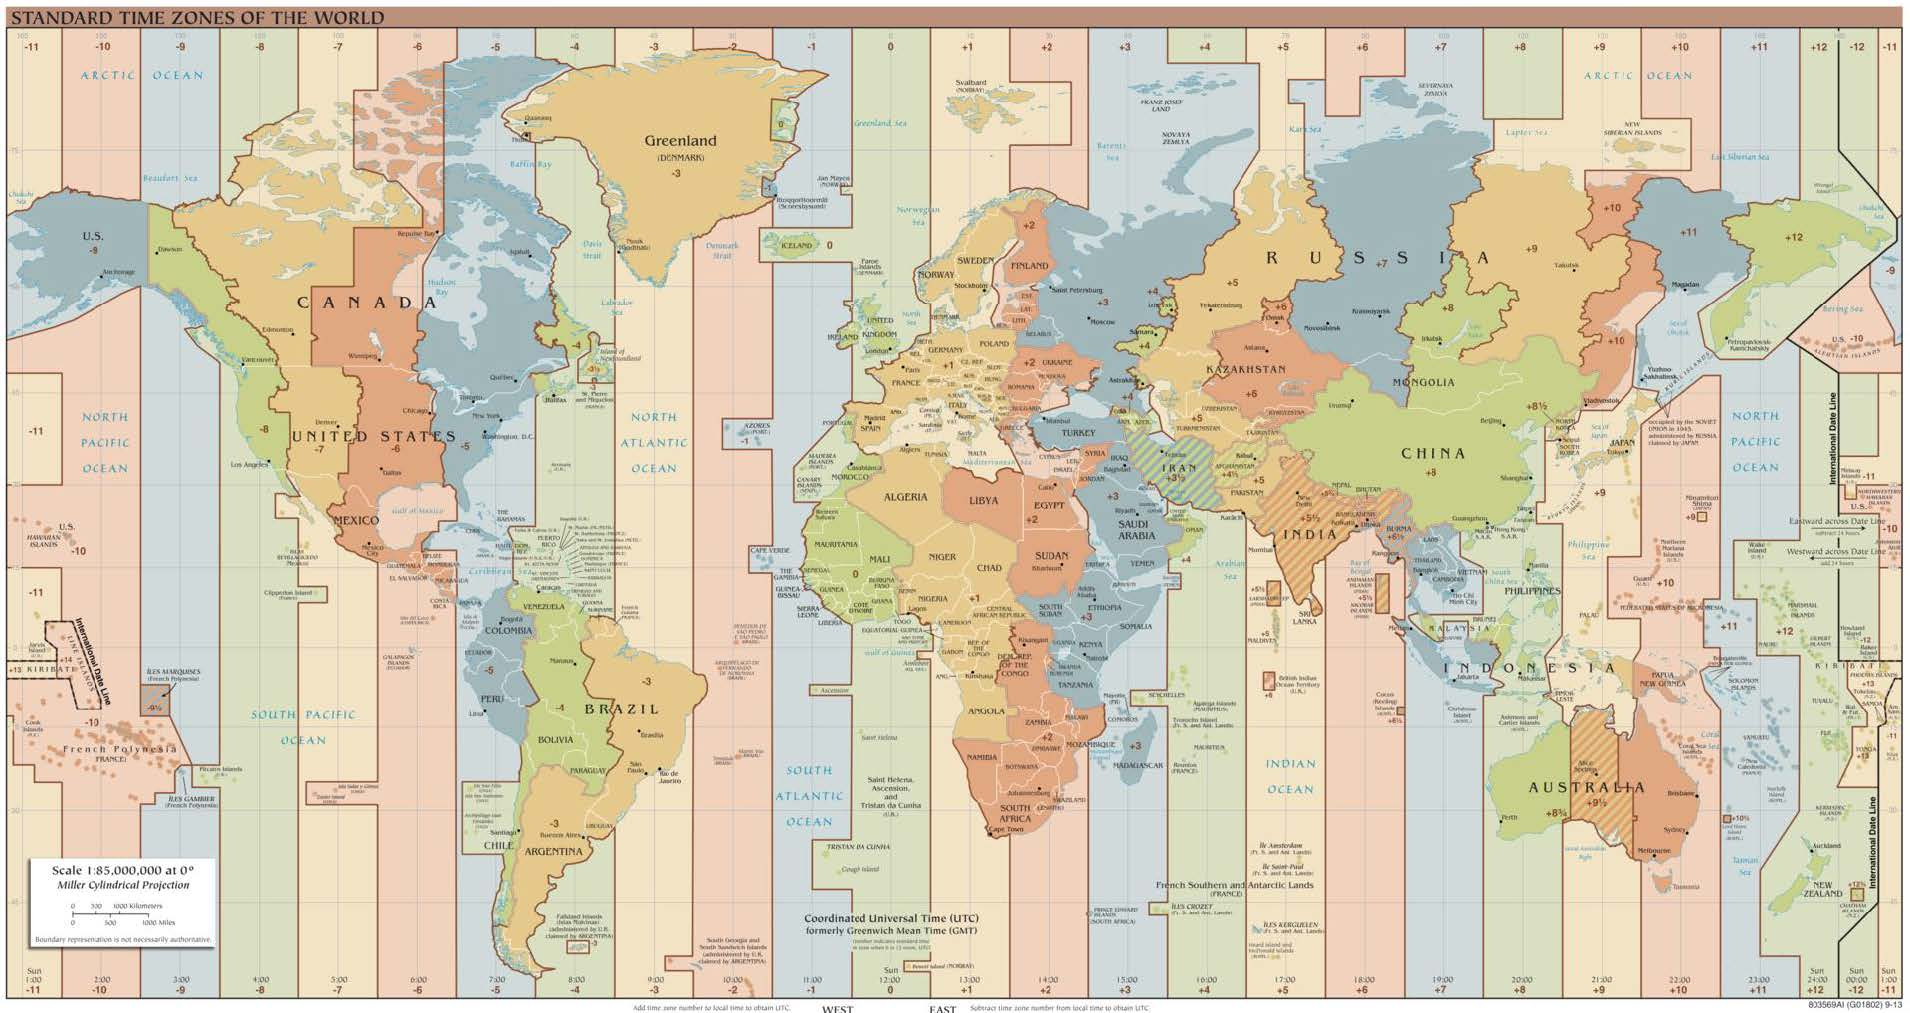
\includegraphics[width=1\textwidth]{images/zeitzonen}
\subsubsection{Zeit in der Geschichte}
Zeit ist kein Naturprodukt, sondern vom Menschen geschaffen. Das Verhältnis des Menschen zur Zeit verändert sich radikal vor allem im Laufe des 19. Jahrhunderts (Industrielle Revolution). Die Eisenbahn und der Telegraph zwingen die Schweiz eine einheitliche Zeit einzuführen und die Lokalzeiten abzuschaffen (Unterschied 18’). 1853 wurde die Berner Lokalzeit für Post und Telegraphie zur einheitlichen Zeit erklärt. 1894 Einführung der mitteleuropäischen Zeit in der Schweiz. Um 1900 dominiert nicht mehr die Sonne sondern die mechanische Uhr das Alltagsleben.
\subsection{Zeitmessung}
1. Phase: bis Ende 13. Jahrhundert -einfache Instrumente ohne Genauigkeit\\
2. Phase: Ende 13. Jahrhundert beginnt die mechanische Zeitmessung
\subsubsection{Geschichte der Messinstrumente, am Beispiel der Uhr}
3000 v. Chr. Sonnenuhren bei den Sumerern und Ägypter. Entwicklung weiterer Uhren in Form von Wasseruhren, Kerzenuhren, Sanduhren und Räucherstäbchenuhren. 3. Jahrhundert v. Chr. entwickeln die Griechen eine erste Uhr mit Hemmungsmechanismus. Im 11. Jahrhundert wurden von arabischen Gelehrten Uhren mit von Wasser angetriebenen Zahnrädern entwickelt. Im Mittelalter brauchten Mönche zuverlässige Zeitangaben um die vorgeschriebenen Gebete zur richtigen Zeit verrichten zu können. Während dem 15. Jahrhundert wurden Sanduhren in der Schifffahrt verwendet. Gleichzeitig wurden in Städten durch Turmuhren die Zeit öffentlich sichtbar gemacht.
\subsubsection{Geschichte der Uhr}
\begin{enumerate}
\item Phase I: bis Ende 13. Jahrhundert -einfach Instrumente ohne Genauigkeit
\item Phase II: Ende 13. Jahrhundert beginnt die mechanische Zeitmessung
\item Phase III: 1657 beginnt die exakte Zeitmessung
\item Phase IV: 1750 beginnt die wissenschaftliche Zeitmessung
\end{enumerate}
Was entscheidet über die Genauigkeit einer Uhr?\\
Regelmässigkeit der periodischen Pendelbewegung, beispielsweise von: Pendeln (Christian Huygens (1629 – 1695), Federn, Quarz, Atom. \\
Ab dem 16. Jahrhundert beginnt man in Europa persönliche Uhren auf sich zu tragen. Mit der Pendeluhr von Hyugens konnte die Genauigkeit der Uhren zuerst auf Minuten, später auf Sekunden verbessert werden. 18. Jahrhundert konnten bereits Abweichungen von Zehntelsekunden festgestellt werden. Pendeluhren blieben bis ca. 1960 als Zeitinstrumente in Dienst. Ab ca. 1960 Quarzuhren ersetzten als Basisinstrumente die Pendeluhren. Später durch Atomuhren ersetzt. Nach 1676 durch den Einbau einer Spiralfeder kann die Genauigkeit bei Taschenuhren verbessert werden. Mit der Fliegerei kam die Armbanduhr auf. 1920er Jahre konnten dank der rotierenden Schwungmasse der automatische Aufzug einführt werden. Dies jedoch nur bei Armbanduhren. In den 30er Jahren gelang es die Armbanduhr stossunempfindlich und unabhängig von der Temperatur zu machen. Ab 1927 die ersten Quarzuhr, die jedoch nur in Laboratorien Verwendung fand. 1938 erste kommerzielle und tragbare Quarzuhr durch Rohde \& Schwarz. 1944 erhält Isidor Isaac Rabi für die Entwicklung der Atomuhr die Nobelpreis. Longines entwickelt 1972 die Digitaluhr. 
\subsubsection{Geschichte der Schweizer Uhrenindustrie}
Ab 1650 mit dem Aufkommen tragbarer Uhren entsteht in der ganzen Schweiz eine Uhrenindustrie mit regionalen Spezifizierungen. In Genf und im Jurabogen Spezialisierung auf tragbare Kleinuhren. Ab 1650 Flucht von Hugenotten nach Genf. Deren Fachwissen kombiniert sich mit der Gold-und Silberschmiedekunst. Um 1690 nur noch Endbearbeitung in Genf – Herstellung der Rohwerkein den benachbarten Juratäler (Verlagssystem). Ab 1779 maschinelle Produktion durch die Idee der Austauschbarkeit von Einzelteilen. Spezialisierung führt zu über 30 verschiedenen Berufen (Verzeichnis 1788). Während der französischen Besetzung Zusammenbruch der Uhrenindustrie. Ab 1850 Konzentration der Uhrenindustrie am Jurafuss(Biel, Grenchen und Solothurn). 1870 produzierte die Schweiz rund 3 Viertel der Weltuhrenproduktion. Durch die industrielle Produktion in den USA faktischer Zusammenbruch der schweizerischen Uhrenindustrie in den 1870er Jahren. Übergang zur maschinelle Serienproduktion ab 1880. Uhrenarbeiter wehren sich gegen die veränderten Arbeitsbedingungen mit Streiks (193 zwischen 1884 und 1914) und der Gründung einer Gewerkschaft 1912 (SMUV, heute Unia). Während dem Ersten Weltkrieg kann die Uhrenindustrie die mangelnde Nachfrage durch die Produktion von Zeitzündern und Munition überbrücken. Aufteilung der Uhrenindustrie in einen Bereich mit der manuelle Endbearbeitung von Luxusuhren und der industriellen Serienproduktion für Uhren in den tieferen Preissegmenten. Um der ausländischen Konkurrenz zu widerstehen wurde die Uhrenindustrie in der Zwischenkriegszeit kartellisiert. 1920 verdrängt die Armbanduhr die bisher übliche Taschenuhr. Durch den Einzug der Elektronik in der Uhrenindustrie halbierte sich die Anzahl der Beschäftigten zwischen 1960 und 1980 von 70‘000 auf ca. 30‘000. 1968 erster Prototyp einer Quarzarmbanduhr. 1980 gleich grosseProduktion mechanischer und elektronischer Uhren. 1982 Swatch als Spritzplastikuhr lanciert und somit Teile der Schweizer Uhrenindustrie gerettet (Nicolas Hayek (1928 – 2010). 2010 exportierte die Schweiz für rund 16.2 Mrd. CHF Uhren. Dies entspricht rund der Hälfte des
wertmässigen Weltuhrenexportes. Von den 2010 rund 1.2 Mrd. hergestellten Uhren kamen rund 26.2 Mio. aus der Schweiz (1.1 Mrd. aus China und Hongkong). Die Uhrenindustrie umfasst rund 600 Unternehmen und ist in der Exportstatistik der Schweiz die drittgrösste Branche.
\subsubsection{Die Schweizer Uhrenindustrie heute}
Die Schweizer Uhrenindustrie produziert rund 2\% der weltweiten Uhrenproduktion. Der Wert der in der Schweiz produzierten Uhren beträgt 53\% der weltweiten Uhrenindustrie (durchschnittlicher Wert einer Uhr: CH 797 \$, HK 35\$, VR China 8\$, D 109\$). Knapp 60‘000 Personen arbeiten in der Schweizer Uhrenindustrie. Sie steuert rund 1.5\% des BIPs der Schweiz bei. Nach der Pharma-und der Maschinenindustrie die drittgrösste Exportbranche. Es gibt rund 500 Unternehmen. Die Hälfte der Schweizer Uhrenexporte geht nach Asien. Zwischen 2000 und 2016 haben sich die Exporte nach China verhundertfacht. Wegen der Anti-Korruptionskampagne der KPChsind die Exporte nach China in den letzten zwei Jahren zurückgegangen. Wer mit 50 keine Rolex besitzt, hat es in seinem Leben zu nichts gebracht. (Jacques Séguéla, Werber in F). Einige wichtige Uhrenfirmen veröffentlichen keine Geschäftszahlen, da sie in Familienbesitz und nicht an der Börse kotiert sind.
\subsubsection{Heinrich Moser (1805 - 1874)}
In Schaffhausen in einer Uhrmacherfamilie geboren. Lehre beim Vater und Weiterbildung in Le Locle. 1827 Auswanderung nach Russland. Kann als Einziger eine Uhr des Zaren reparieren. 97\% der Auswanderungen nach Nord-/Süd-Amerika (Passabgabe, nicht best-ausgebildet). 3\% der Auswanderungen nach Russland (gut ausgebildet). 1828 Gründung eines Uhrenhandelsgeschäfts in St. Petersburg – später Zweigniederlassungen in der Schweiz. 1848 Rückkehr in die Schweiz. 1851 Rheinkanal fertiggebaut. 1853 Mitbegründer einer Waggon-Fabrik, der später SIG, und der Rheinfallbahn (Winterthur- Schaffhausen). 1866 Bau eines Wasserkraftwerks – Industrialisierung. 1868 Mitbeteiligt an der Gründung der IWC.
\section{Medizin}
\subsection{Wie entwickelten sich die Kenntnisse über den menschlichen Körper?}
Bis ins 17. Jahrhundert beriefen sich die Mediziner immer noch auf die Theorien von Galen von Pergamon (129 – 210). (Das Blut wird zur Ernährung von den Organen angesaugt. Das Blut bewegt sich in Sackgassen (den Venen) von der Leber in die Glieder, wo es verbraucht wird. Humoralpathologie (Viersäftelehre).)  Arabische Mediziner bewahren das antike Wissen – im Westen Kräuterkunde. Um 1500 wurden die Kenntnisse durch das Sezieren von Leichen vergrössert. 1628 postulierte der Engländer William Harvey den doppelten Blutkreislauf. Somit konnte das zirkulierende Blut als Transport- und Verteilmedium für Arzneimittel genutzt werden. Staat übernimmt aus politischen Gründen immer mehr Funktionen in der Medizin (Universitäten). Die universitäre Medizin konnte immer grösseren Einfluss ausüben und andere Berufsgruppen (Hebammen, Bader, usw.) verdrängen. Im 18. und 19. Jahrhundert erfolgten weitere Entdeckungen, wie beispielsweise die Nerven. Im 19. Jahrhundert konnten viele Erreger von Seuchen entdeckt und somit bekämpft werden. Durch die verbesserte Hygiene konnten zahlreiche Infektionskrankheiten, speziell in der Chirurgie, besiegt werden. Mit der Entdeckung der Röntgenstrahlen und der Radioaktivität konnten zusätzliche Anwendungen in der Diagnostik und der Therapie angewandt werden.\\
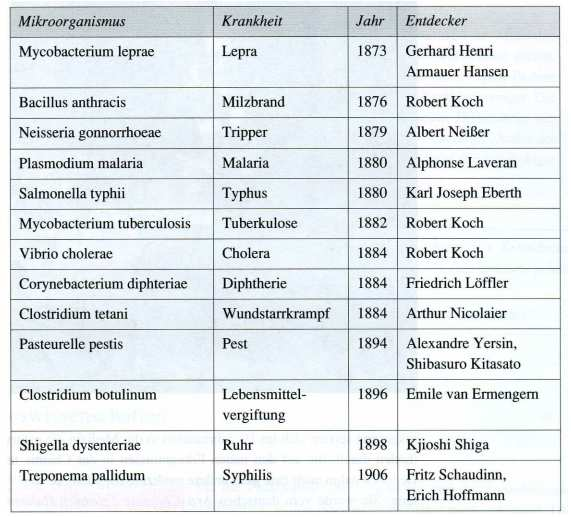
\includegraphics[width=.5\textwidth]{images/krankheit}\\
Einfluss auf mächtige Personen (Seuchen, körperlicher \& mentaler Verfassung):\\
\begin{tabular}{l l}
Bloody Mary & 5 Jahre an Macht (bevor Tod durch Infektion) $ \rightarrow $ 100te \glqq Berater\grqq verbrennen\\
Schwarzer Tod & Beulenpest Mitte 14. Jahrhundert $ \rightarrow $ 1/3 europäischer Bevölkerung starb\\
Napoleon & Schlacht von Waterloo, Burnout-Syndrom (unter Opiate)\\
Kaiser Wilhelm II & psychisch labile, unsichere Persönlichkeit (Verkrüppelung linker Arm)\\
Sir Edward Grey & litt unter beginnender Blindheit: \glqq In Europa gehen die Lichter aus, und wir werden \grqq \\
& sie zu Lebzeiten nicht mehr angehen sehen! \\
Heutzutage & Krankheiten etc. werden vertuscht (John F. Kennedy, Francois Mitterrand)\\
Durch Demokratie & Einfluss des Staatsgeschickes nicht auf einzelne Personen verteilen
(Schutzmechanismus)\\
\end{tabular}
\subsection{Bedeutende Ärzte}
\subsubsection{Hippokrates von Kos (460 – 370)}
\begin{wrapfigure}[4]{r}{2cm} 
\vspace{-1.5cm}
  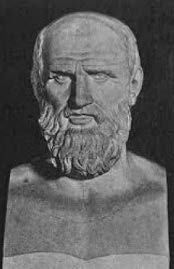
\includegraphics[height=2.5cm]{images/hypokrates}
\end{wrapfigure}
Entstammte einer Ärztefamilie. Ihm werden 61 Schriften zugeschrieben. Versucht er die Medizin auf eine vernunftmässige Beobachtung der Natur zu stellen. Hyppokratische Säftelehre zentral (Blut, Schleim, gelbe und schwarze Galle). Der Eid des Hippokrates ist das erste sittliche Grundgesetz für die Ärzte. \clearpage
\subsubsection{Paracelsus (Bombastus von Hohenheim) (1493 (Egg, SZ) – 1541 (Salzburg))}
\begin{wrapfigure}[7]{r}{2cm} 
\vspace{-0.5cm}
  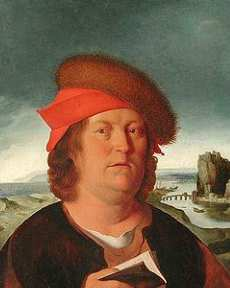
\includegraphics[height=2.5cm]{images/paracelsus}
\end{wrapfigure}
Studium der Medizin in Basel und Wanderjahre. Dozententätigkeit an der Universität Basel – Vorlesungen auf Deutsch. Medizin hat auf Natur- und Gotteserkenntnis sich zu stützen. Kritik an der Humoralpathologie – dafür Erklärungen der Krankheiten durch: Ens Astrorum, Ens Veneni, Ens Naturale, Ens Spirituale, Ens Dei. \glqq Alle Dinge sind Gift, und nichts ist ohne Gift; allein die Dosis macht es, dass ein Ding kein Gift ist\grqq .Ursachen der Krankheiten ist die Ungleichheit der Grundsubstanzen: Schwefel, Quecksilber und Salz. Geschlechterunterschiedliche Arzneien. Stellte eine neue Ernährungslehre auf – bei der der Zucker in den Nachtisch verschoben wird. 
\subsubsection{John Snow (1813 – 1858)}
\begin{wrapfigure}[6]{r}{2cm} 
\vspace{-0.5cm}
  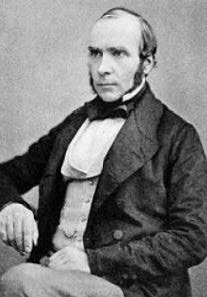
\includegraphics[height=2.5cm]{images/snow}
\end{wrapfigure}
Entstammte ärmlichen Verhältnissen. Ausbildung bei einem Apotheker und Arzt. Studium in London – Abschluss als Arzt und Apotheker. Wegweisende Entwicklung beim Narkoseverfahren. Erkannte die Übertragung der Cholera nicht über Dünste (Miasmen) sondern durch Mikroorganismen im Trinkwasser. Dadurch gelang es ihm die Cholera Epidemie von 1854 in London zu stoppen. 
\subsubsection{Wilhelm Conrad Röntgen (1845 – 1923)}
\begin{wrapfigure}[6]{r}{2cm} 
\vspace{-1.5cm}
  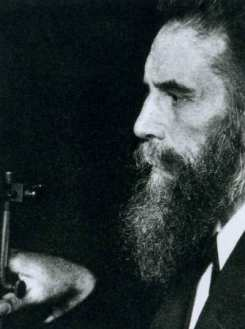
\includegraphics[height=2.5cm]{images/roentgen}
\end{wrapfigure}
Deutscher, Jugendjahre in den NL verbracht. Aus disziplinarischen Gründen von der Schule verwiesen. 1865 – 1868 Studium Maschinenbau an der ETH Zürich, 1869 Promotion in Physik an der Universität Zürich. Professor für Physik in Strasbourg. 1895 Entdeckung der X-Strahlen. 1901 Nobelpreis für Physik. Verzichtete auf die Patentierung des Röntgenapparats. Seine Entdeckungen führten zur Entdeckung der Radioaktivität.
\subsubsection{Alexander Fleming (1881 – 1955)}
\begin{wrapfigure}[3]{r}{2cm} 
\vspace{-1.5cm}
  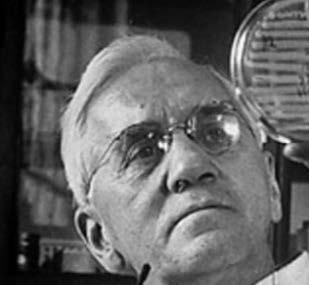
\includegraphics[height=2.5cm]{images/fleming}
\end{wrapfigure}
Bauernsohn in Schottland. Studium der Medizin – akademische Laufbahn. 1921 entdeckte er das Lysozym. 1928 bemerkte er zufällig die keimtötende Wirkung des Penicillium. 1944 geadelt und 1945 den Nobelpreis erhalten. Karriere in der Freimaurerei.
\subsubsection{Rolf Zinkernagel (*1944)}
\begin{wrapfigure}[4]{r}{2cm} 
\vspace{-1cm}
  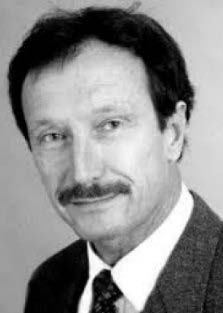
\includegraphics[height=2.5cm]{images/zinkernagel}
\end{wrapfigure}
Studium der Medizin in Basel. Dozententätigkeit in Australien und Zürich. Entdeckte 1973 wie das Immunsystem infizierte Zelle erkennt. Erhielt dafür 1996 als 24. Schweizer einen Nobelpreis.
\section{Kulturepochen}
\subsection{Grundsätzliche Überlegungen}
Je nach den gesellschaftlichen Situationen möchte der Mensch von seiner Umwelt bescheiden oder dominant wahrgenommen werden. Die Modeströmungen wechseln sich dauernd ab. Es bleiben Dinge nur immer dann erhalten, wenn der Mensch keine finanziellen Möglichkeiten hat, die weiteren Modeströmungen mitzumachen. Nach einer gewissen Zeitepoche findet der Mensch alle Dinge schön. Die Behausung und die Kleidung sind Zeichen gegen aussen, wie der Mensch wahrgenommen werden möchte. (\glqq Kleider machen Leute\grqq Gottfried Keller)
\subsubsection{Bedürfnisse - Bauten}
\begin{tabularx}{1\textwidth}{L{6cm}   X}
\rowcolor[gray]{.6} \textbf{Bedürfnis} & \textbf{Bauten} \\ 
Schutz & Burg \\
\rowcolor[gray]{.9} Macht zelebrieren / repräsentieren & Schloss\\
Glaube & Kirche / Kathedrale / Klöster \newline hoher Turm = möglichst nahe an Gott\\
\rowcolor[gray]{.9} Mobilität & Strassen, Eisenbahn, Kanäle, Häfen\\
Licht & Grosse Fenster\\
\rowcolor[gray]{.9} Ideologie sichtbar machen & Kapitol, Reichstagsgebäude\\
Wirtschaftlicher Erfolg zeigen & Paläste (Stadt / Unternehmen)\\
\rowcolor[gray]{.9} Technische Entwicklung & Eiffelturm, Bahnhofshallen\\
\end{tabularx}
\subsection{Die verschiedenen Kulturepochen – Bauten}
\subsubsection{750-1250 Romanisch}
Wissenschaft-Weitergabe über Klöster (Schreiben, Lesen, Wissen, etc.). Grosse Fenster = Luxus. \\
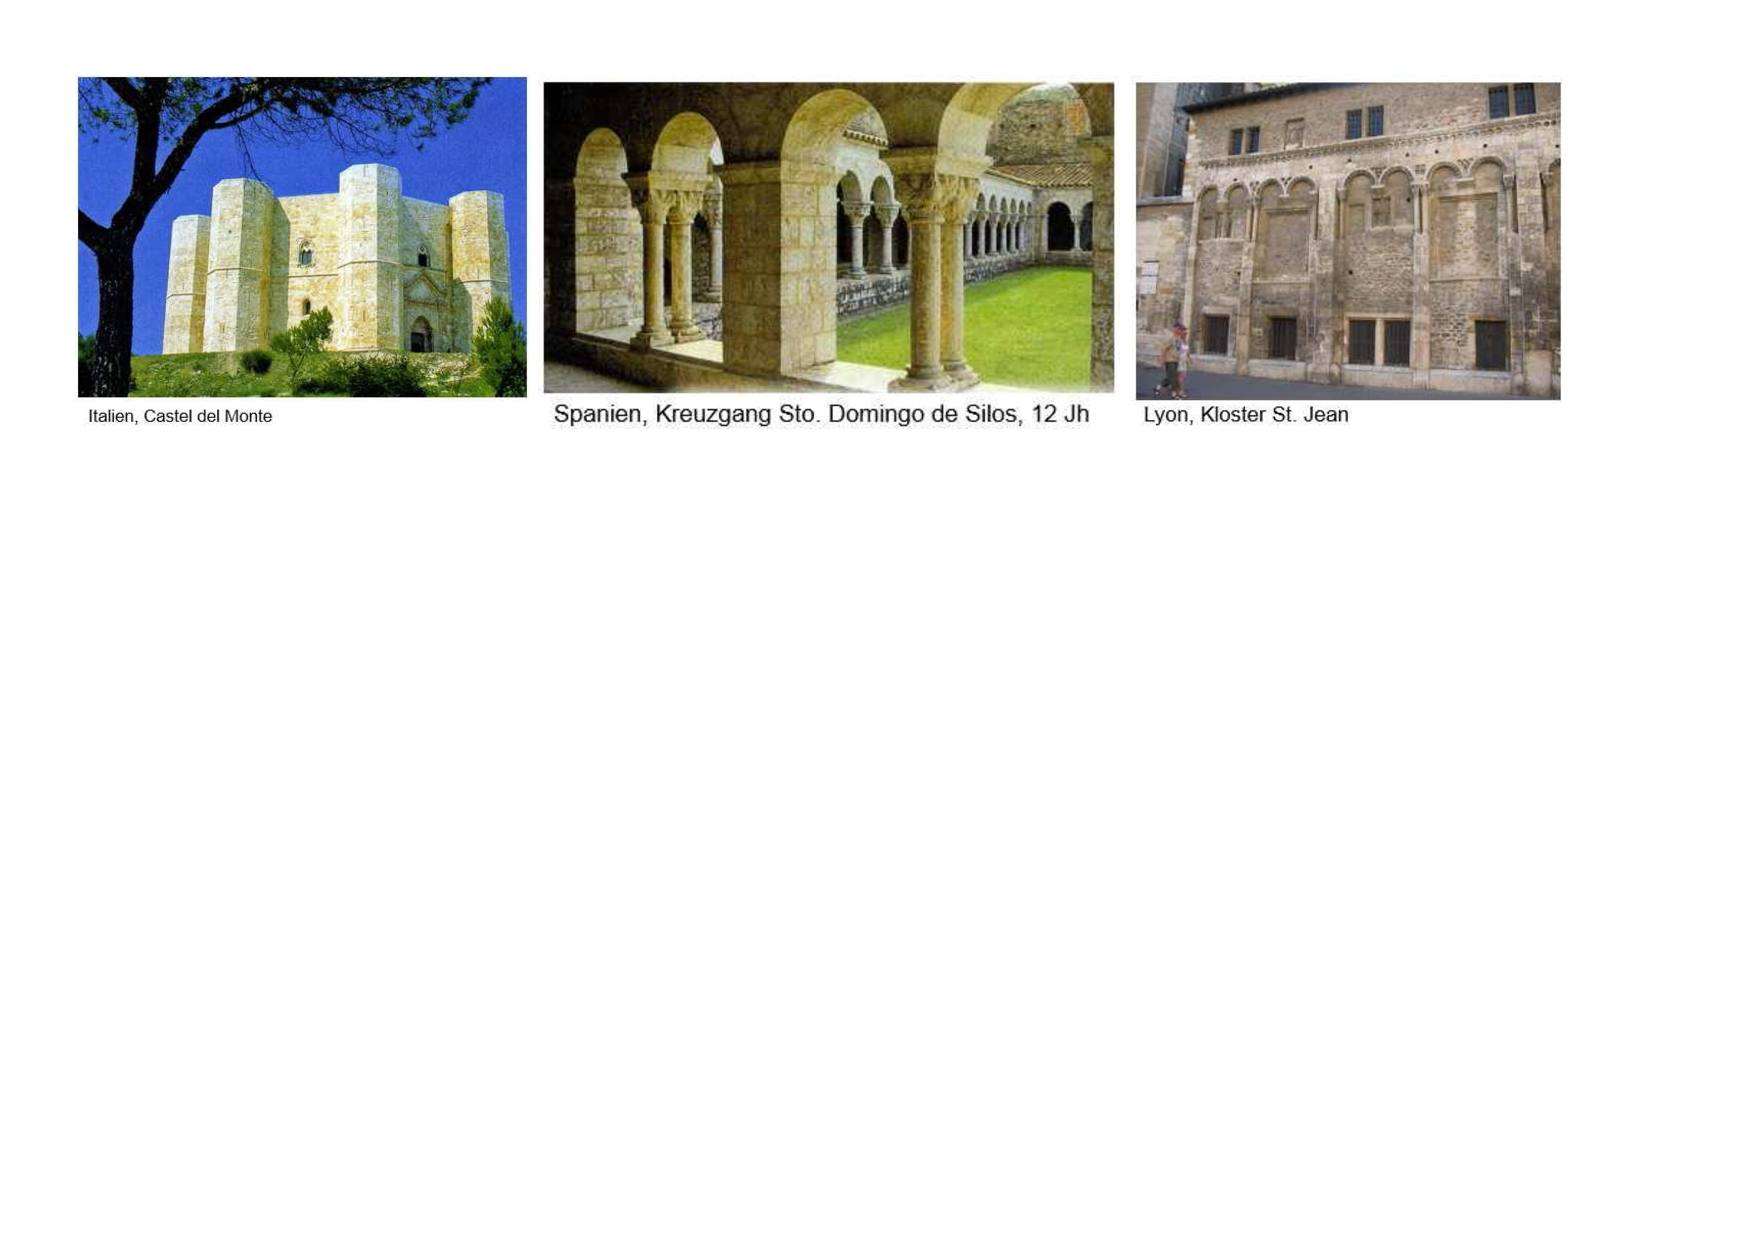
\includegraphics[width=1\textwidth]{images/romanisch}
\subsubsection{1130-1500 Gotik}
Bessere technische Möglichkeiten (Wettkampf um Turmhöhe). Zeit der Kathedralen (zB Notre Dame in Paris). Stadt im Zentrum des Lebens.\\
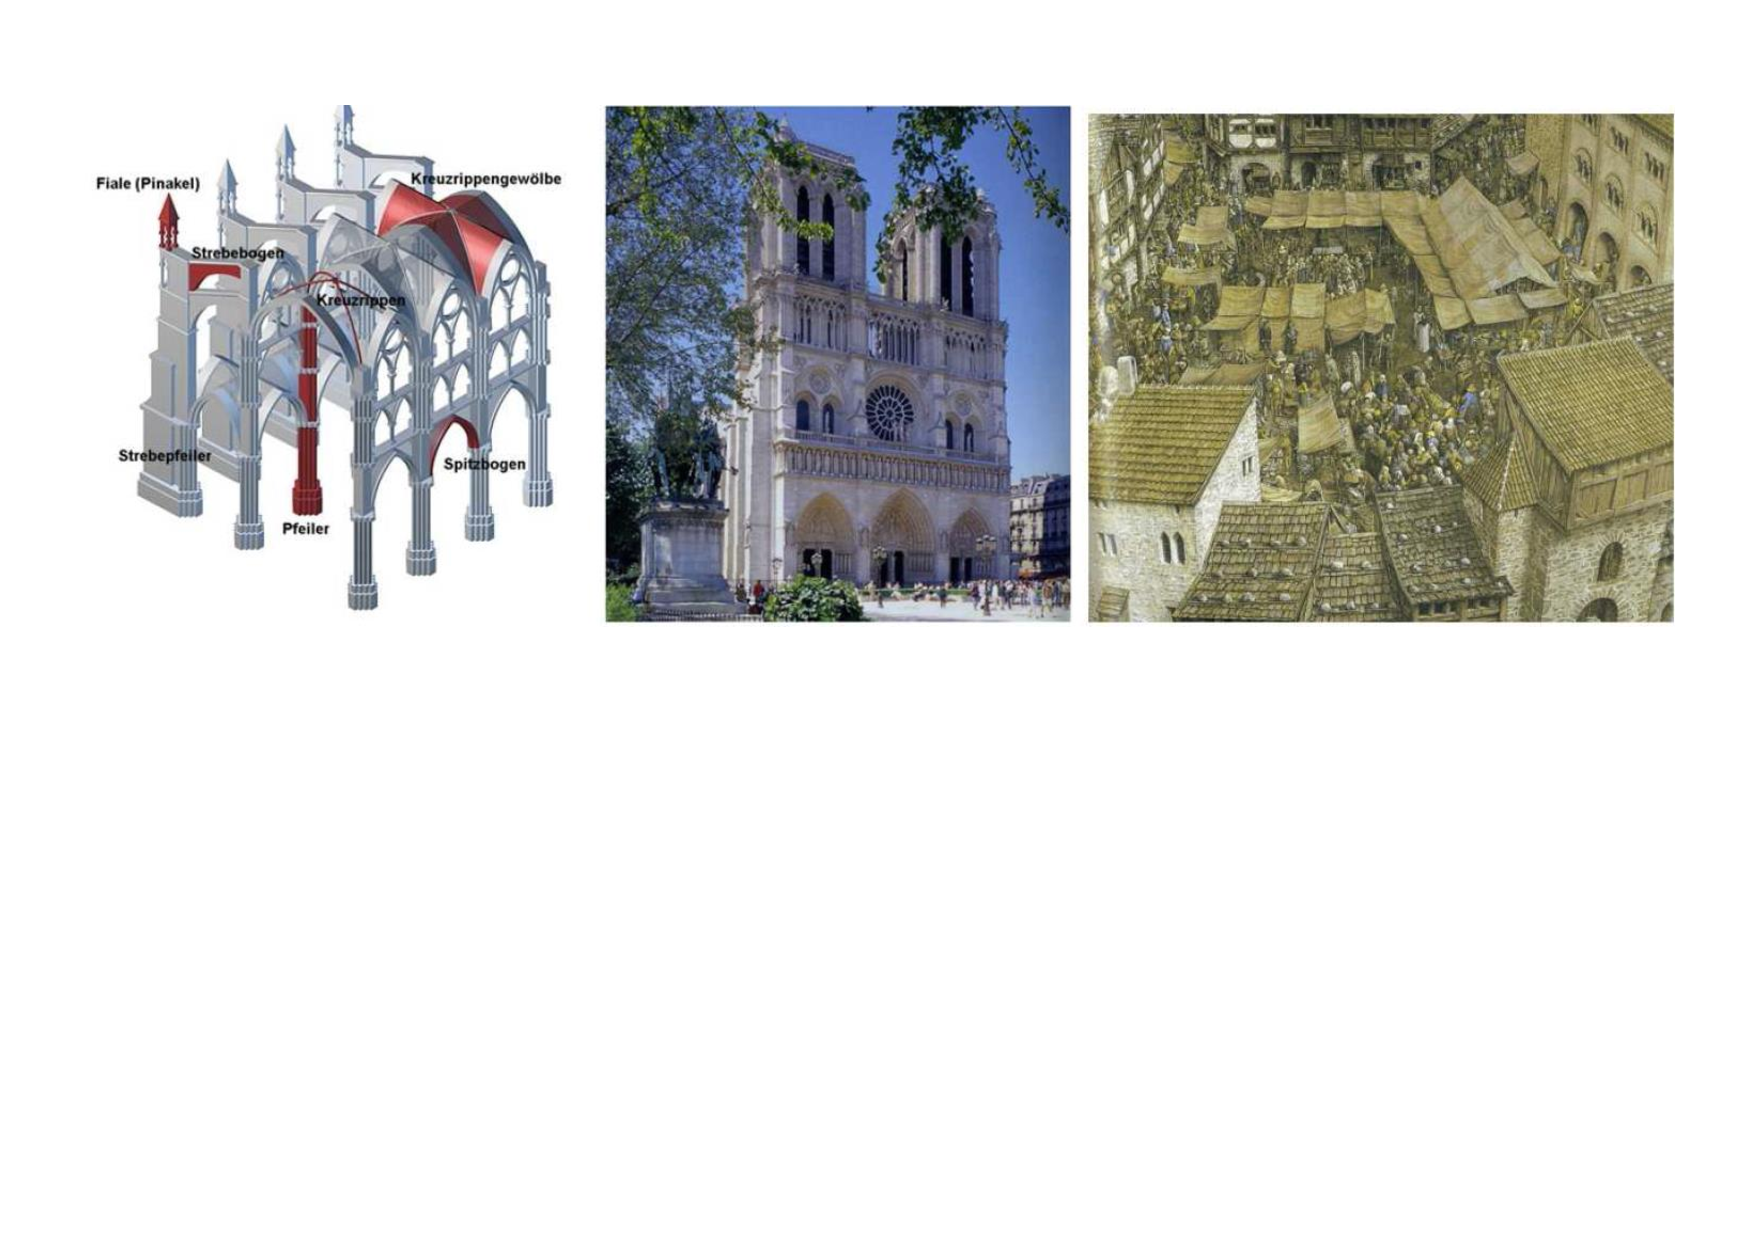
\includegraphics[width=1\textwidth]{images/gotik}
\subsubsection{1420-1620 Renaissance}
Den Menschen geht es besser $ \rightarrow $ 1500 zurück in die Antike (Betonung des Individuums). Sie können sich von den Gedanken ans Jenseits lösen - das Diesseits wird bedeutender. Beginn der Säkularisierung des Denkens. Kulturelle Blühte vor allem in den italienischen Städten. Adel verliert an Macht – Bürgertum in den Städten wird mächtiger und selbstbewusster. Die Menschen beginnen ihre Macht auch äusserlich darzustellen / zu demonstrieren. König im Zentrum (Kirche als Mittel dem König Macht zu geben von den Bürgern). \\
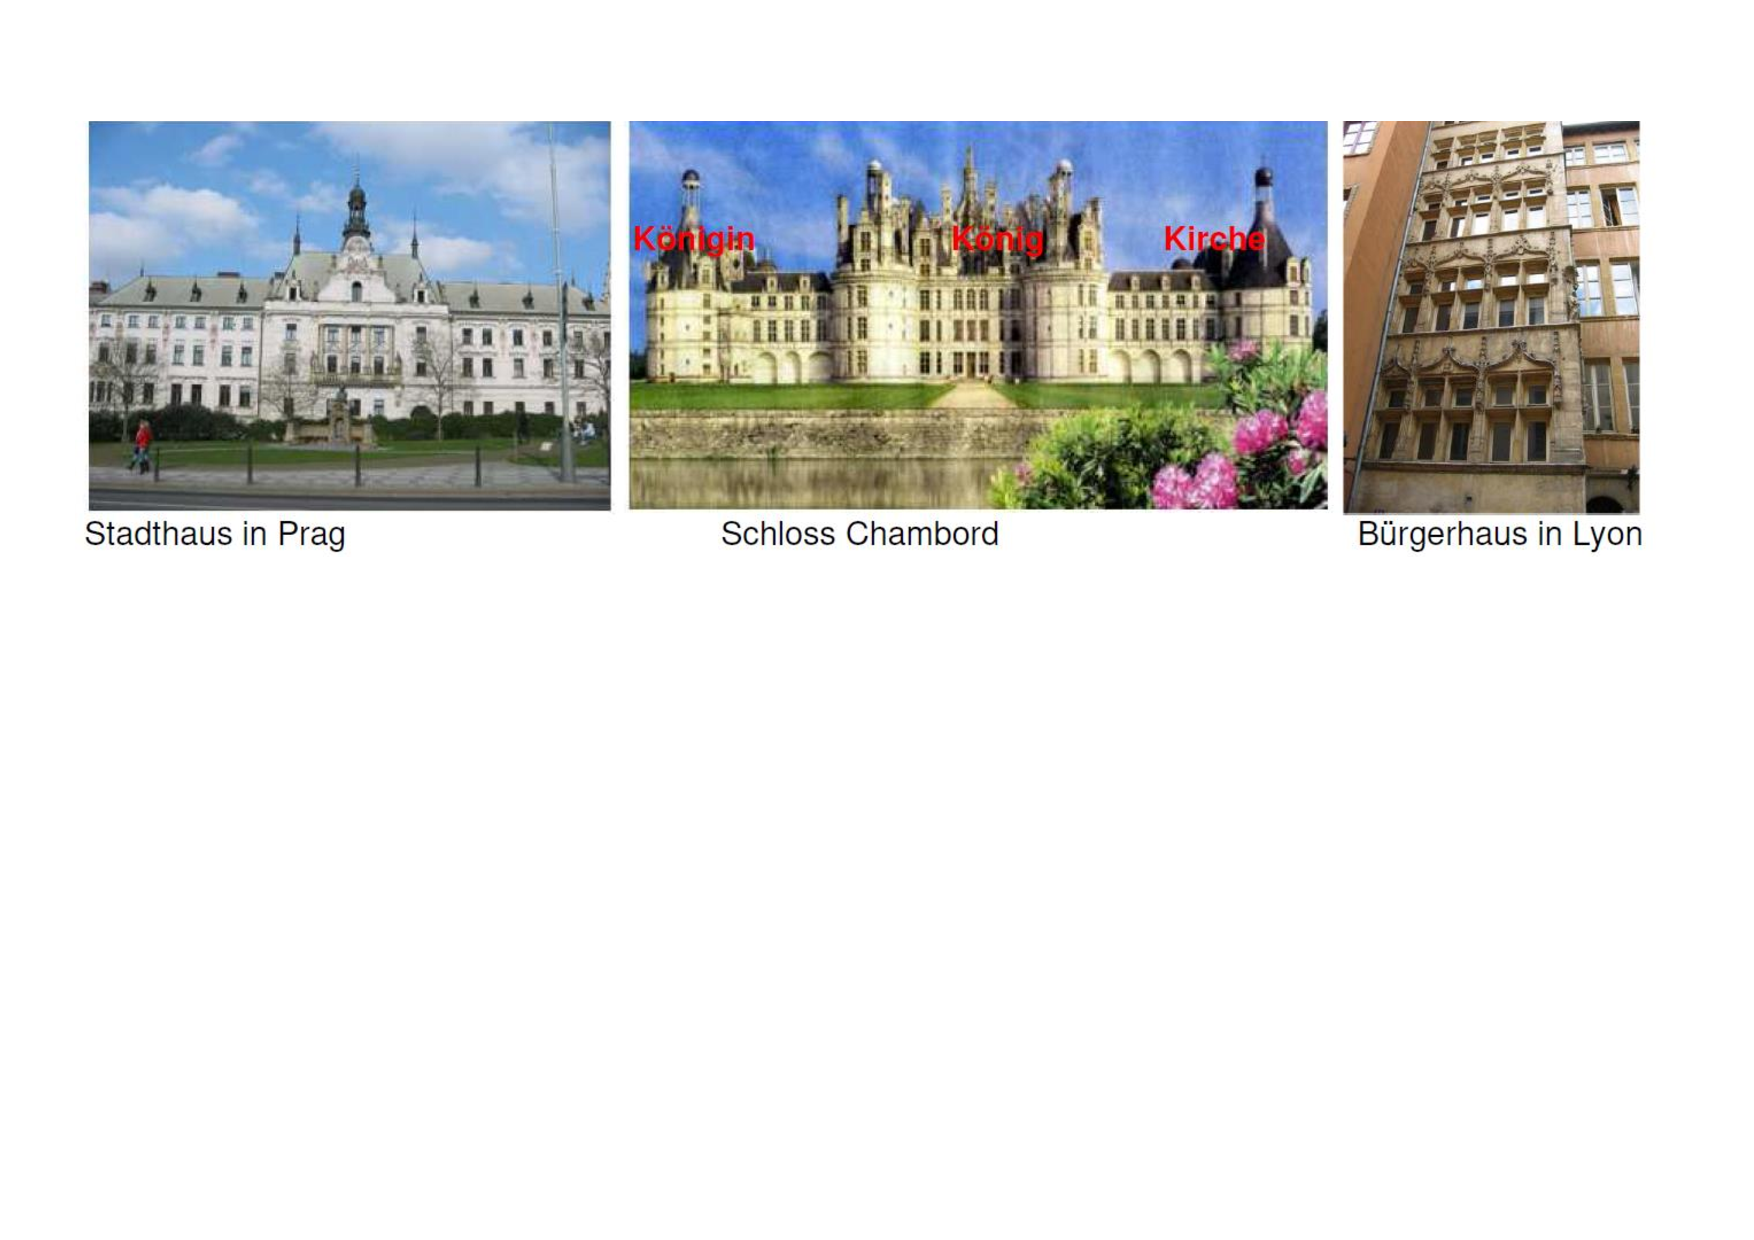
\includegraphics[width=1\textwidth]{images/rennaissance}
\subsubsection{1600-1780 Barock/Rokoko}
Die Könige werden wieder stärker. Die (katholische) Kirche wird wieder mächtiger. Unterschiedliche Baustile in protestantischen und katholischen Gebieten. Leitsatz: Mehr Schein als Sein. Alles ist in Bewegung. Auch der Raum wird in die Bauten einbezogen – Garten. Rokoko als Spätbarock – mit lieblichen Farben. Decken aus Stoff, Spiegel $ \rightarrow $ Raum wirkt grösser, Kleider \& Perücken. Geplante Gärten (so schön wie Schloss) $ \rightarrow $ Zeigen: Beherrschung der Natur. Feuerwerk + Fontänen $ \rightarrow $ nicht nötig (nur Macht demonstrieren). Kirche wird hinterfragt $ \rightarrow $ Beweisen, dass sie stark sind $ \rightarrow $ Bauten erstellen. \\
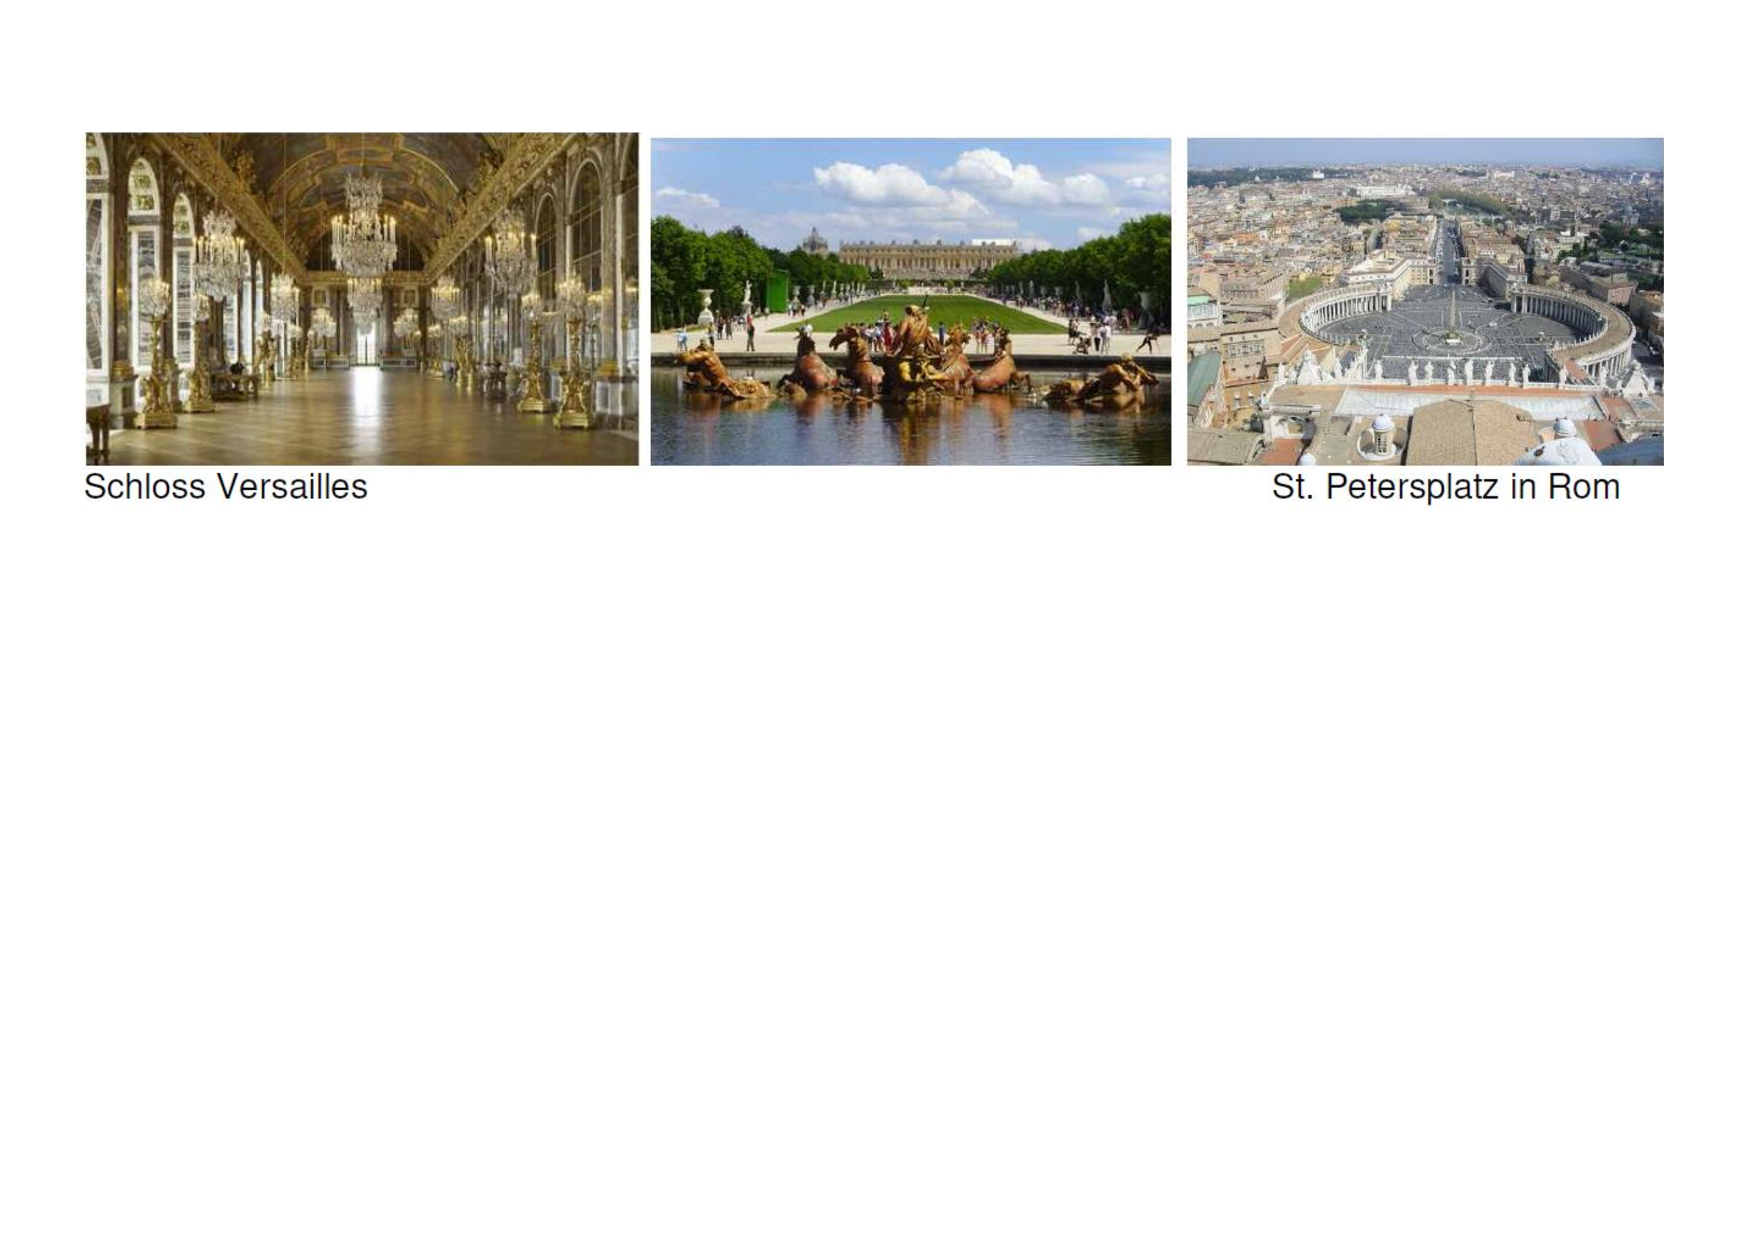
\includegraphics[width=1\textwidth]{images/barock1}
\subsubsection{1750-1840 Klassizismus}
Baustil der Aufklärung. Mit menschlicher Vernunft bauen. Eher die protestantische – republikanische Bauweise. Bauweise des modernen Staates. Rückbesinnung auf die griechische und römische Antike.\\
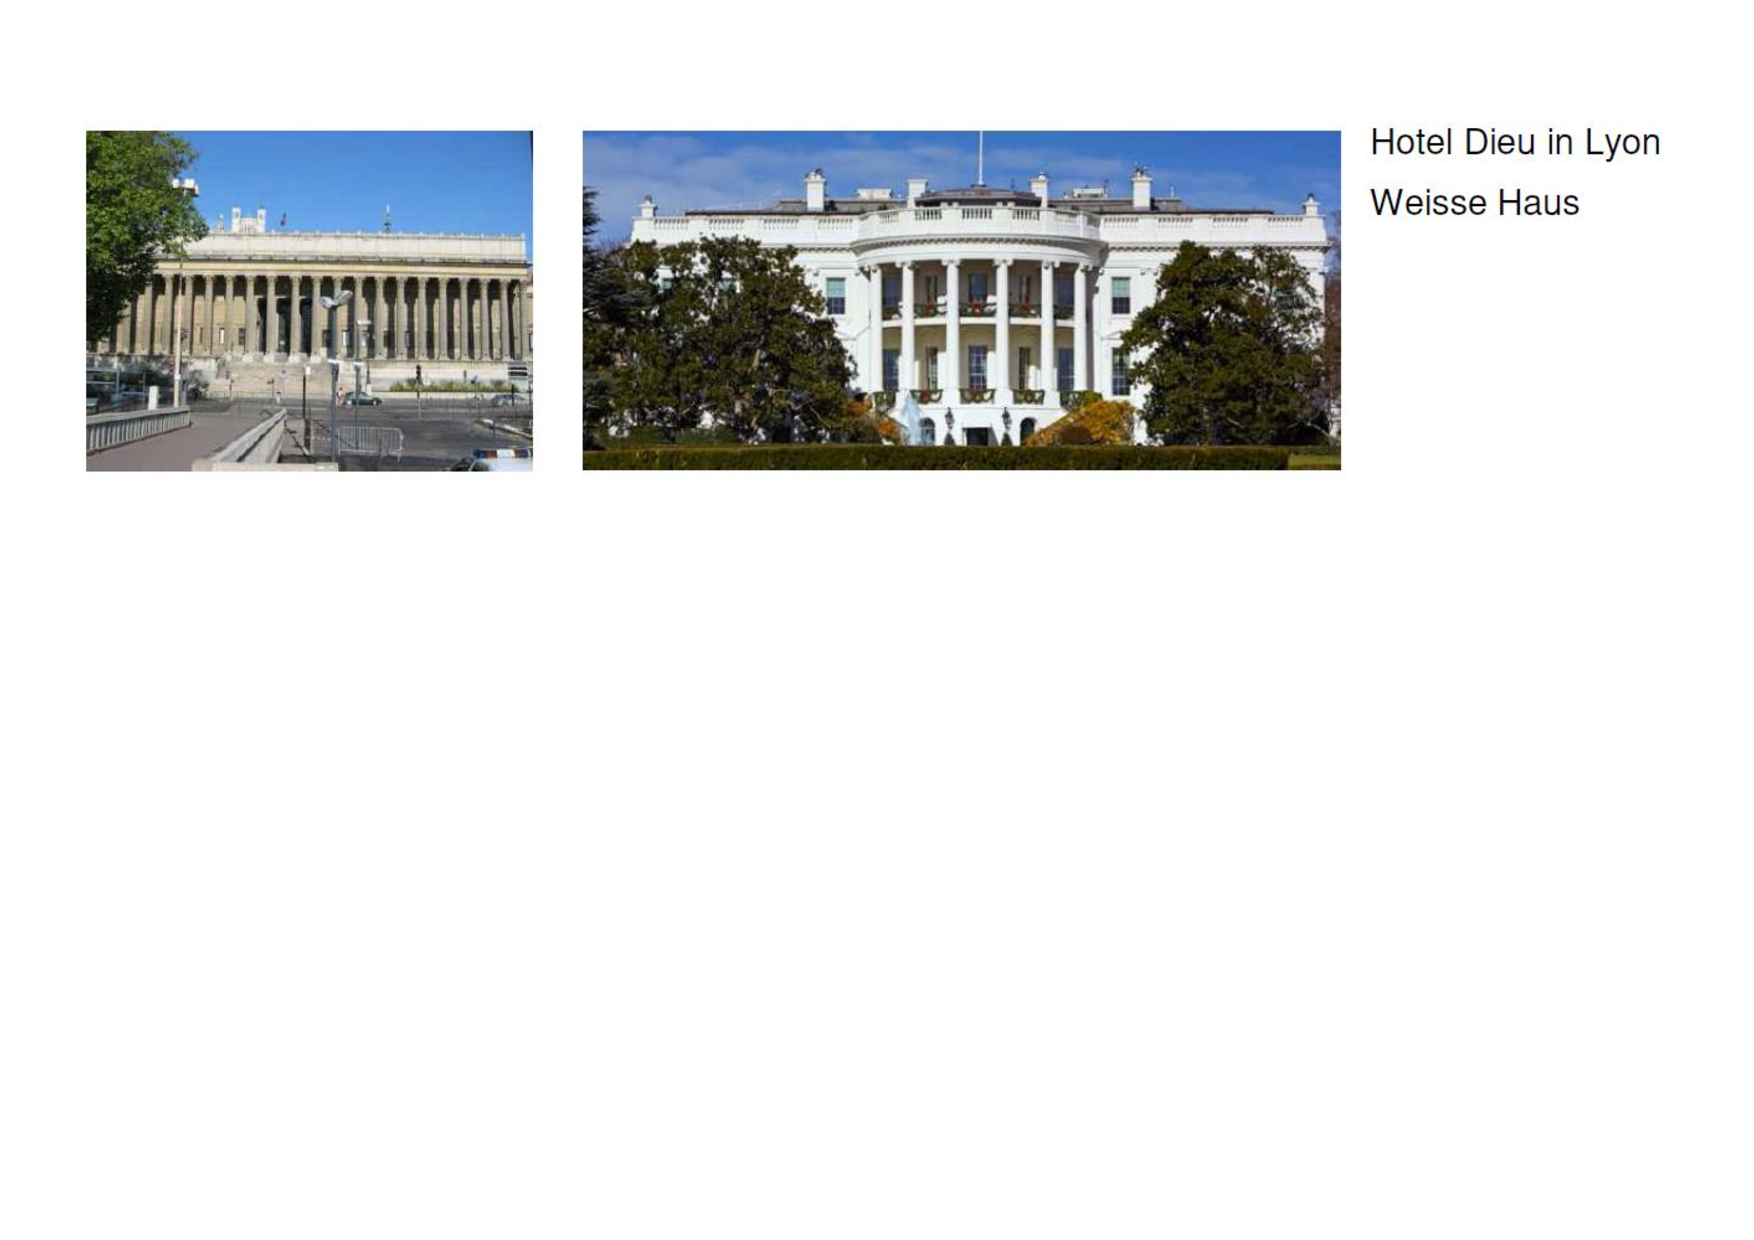
\includegraphics[width=1\textwidth]{images/klassizismus}
\subsubsection{1840-1900 Historismus (Ingenieur-Architektur)}
Die Welt ändert sich viel zu schnell – Blick in die \glqq schöne - heile\grqq Vergangenheit. Neue technische Möglichkeiten. Es gibt die Neo-Gotik, Neo-Renaissance, usw. aber auch Gebäude mit einer Mischung aus allen bisherigen Baustilen (Alle bisherigen Baustile vereint).\\
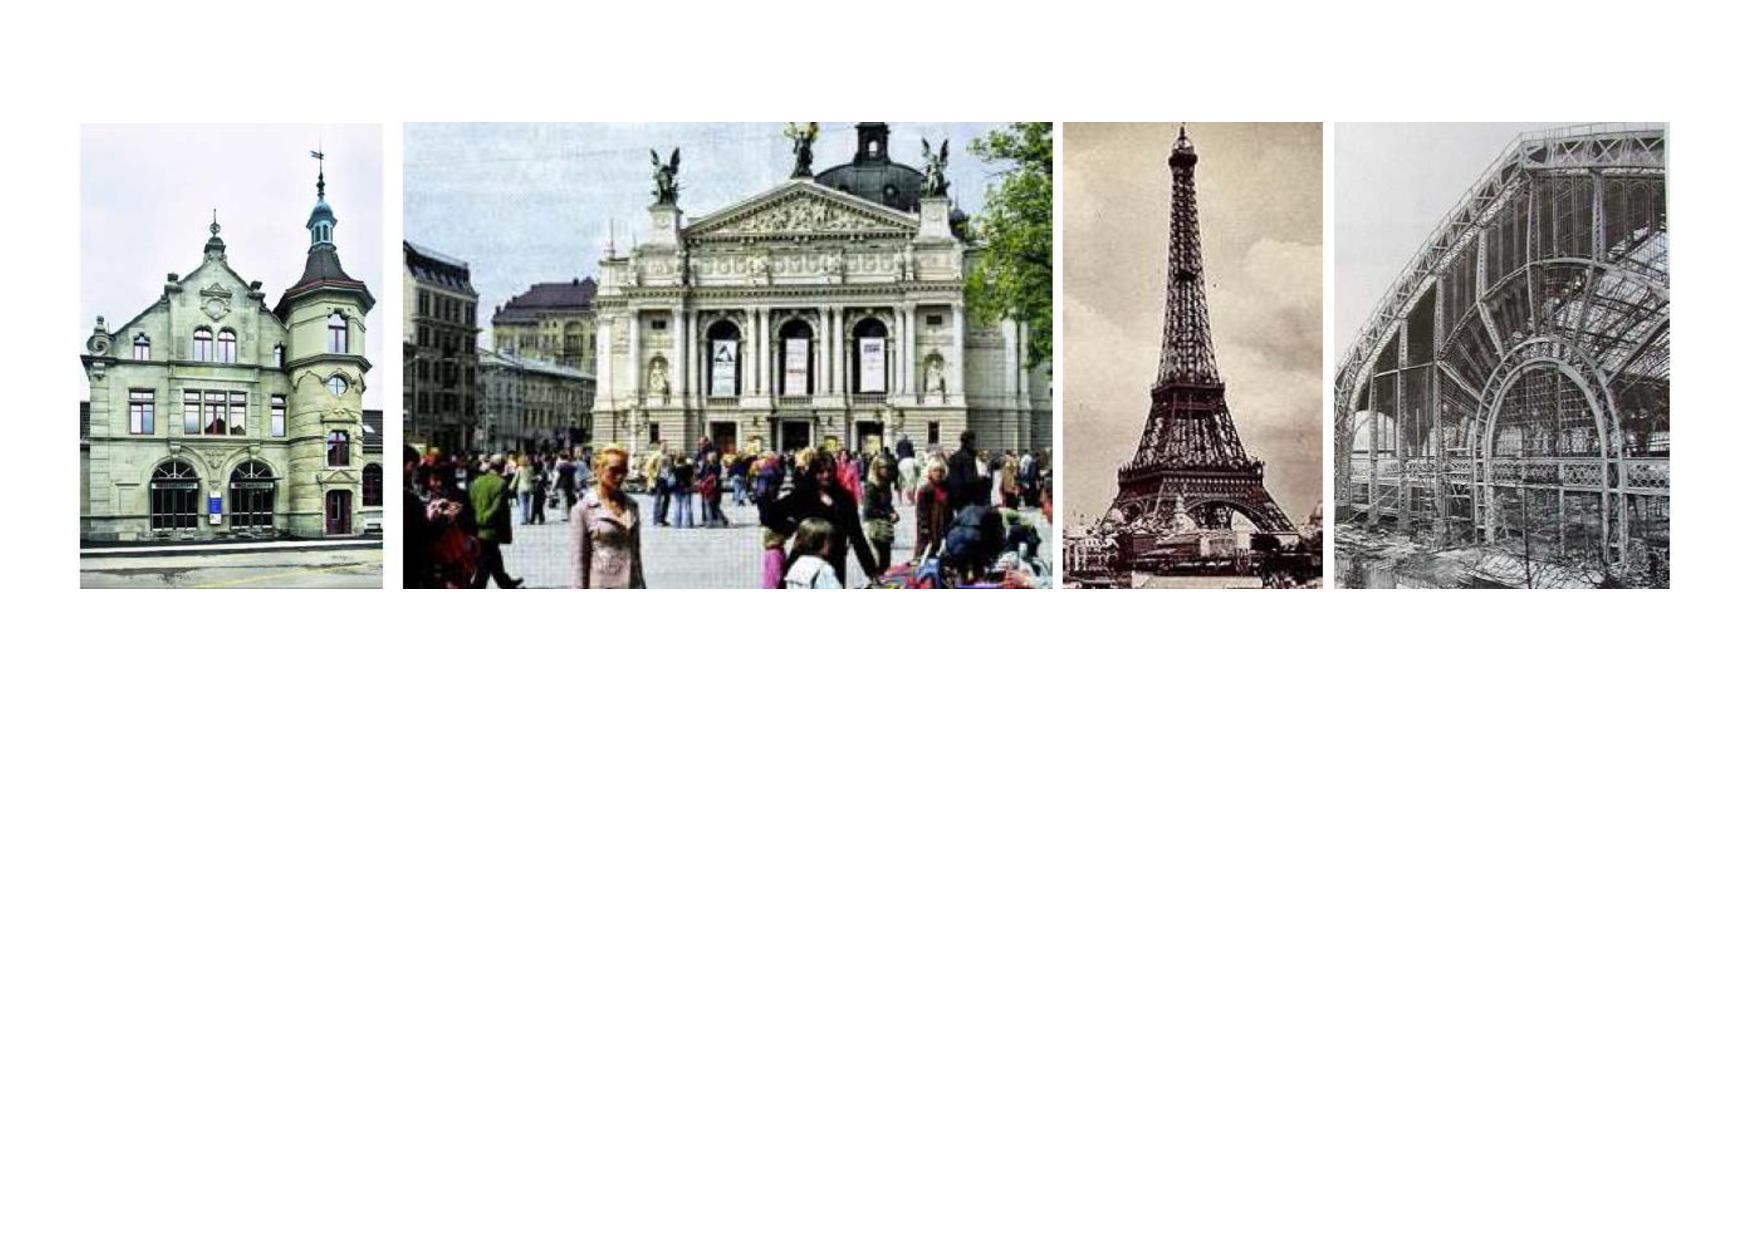
\includegraphics[width=1\textwidth]{images/historismus}
\subsubsection{1900- 1950 Jugendstil/Futurismus/Kubismus/Bauhaus}
Alles ist erlaubt – welche Regeln gelten noch? Dem Bauen sind \glqq keine\grqq technischen Grenzen mehr gesetzt. Mehr Farbe – mehr Lieblichkeit. Mehr aus Materialien und nicht Gemälde (Bsp. Metall- / Glas-Blume). \\
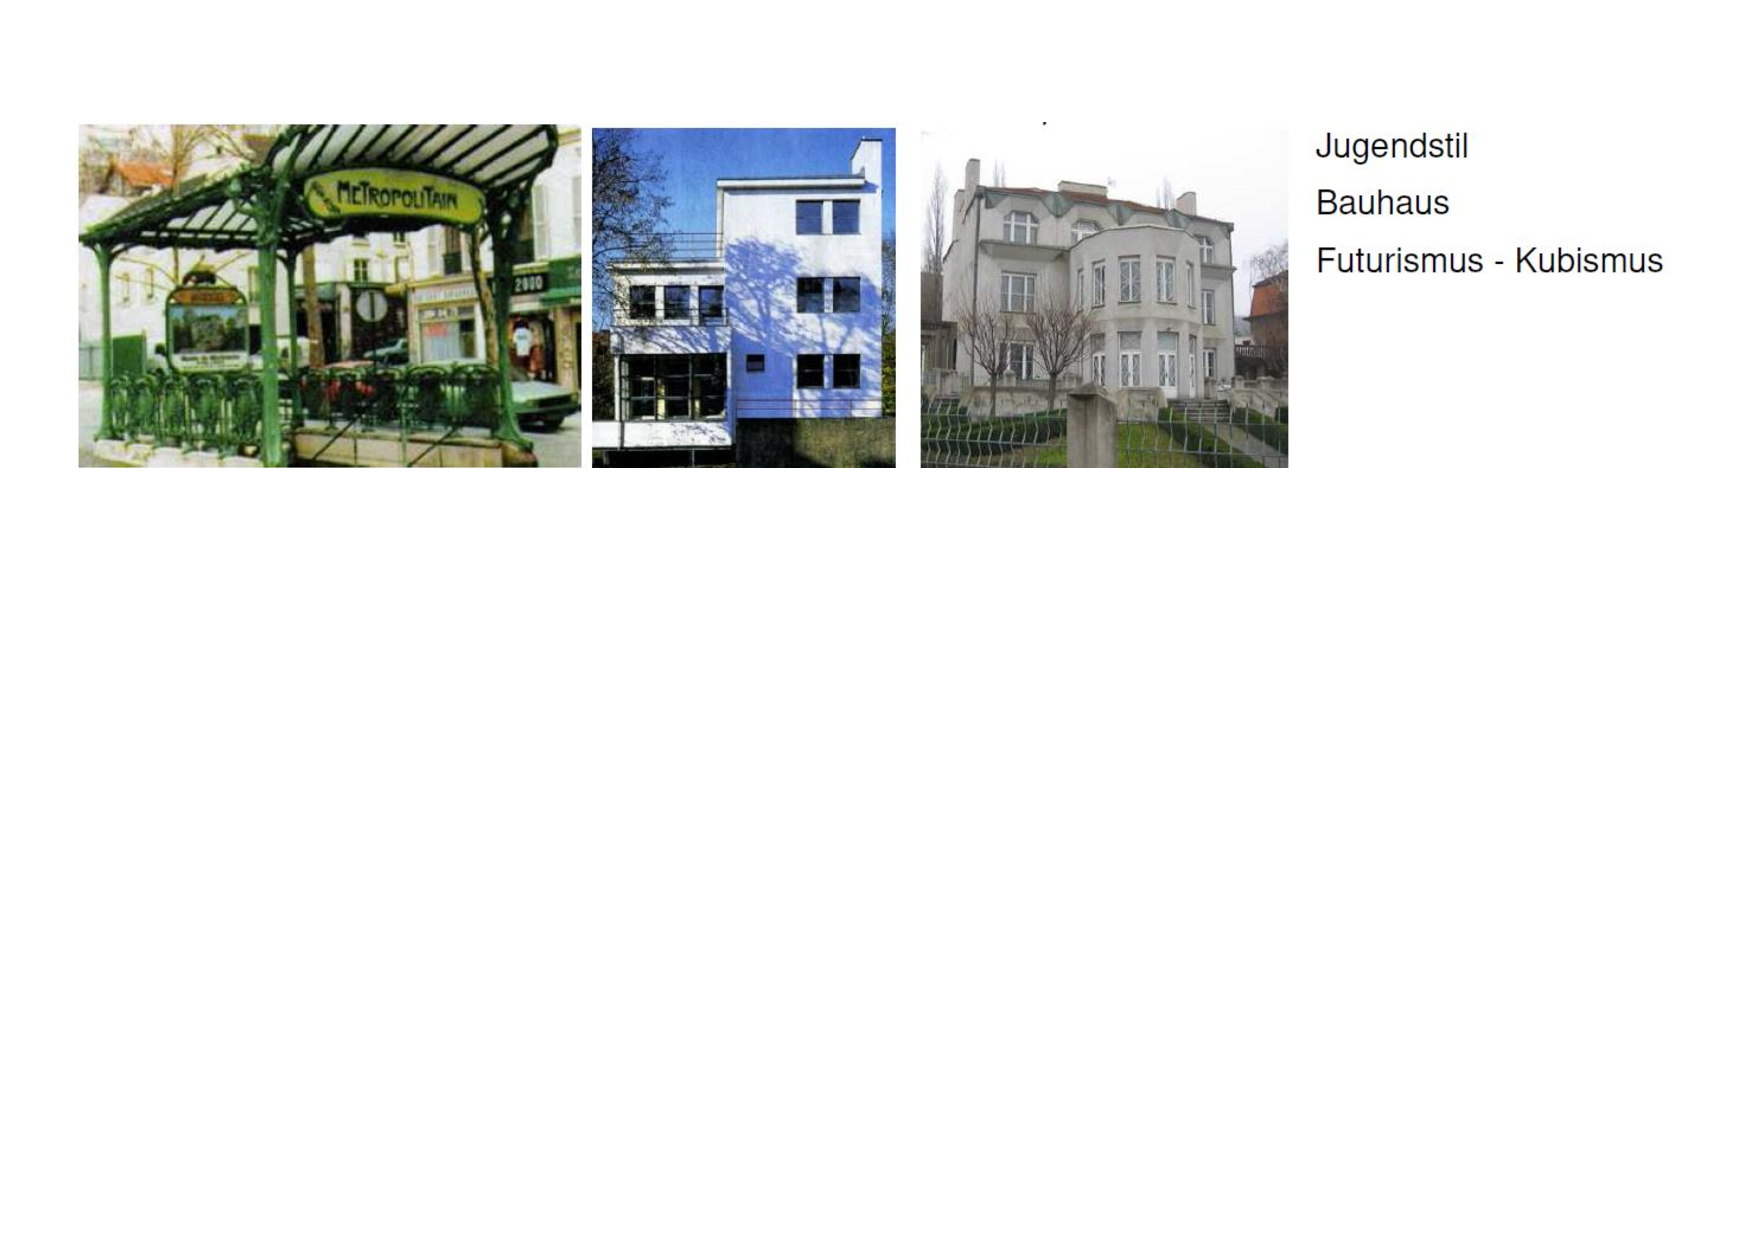
\includegraphics[width=1\textwidth]{images/jugendstil}
\subsubsection{Ab 1950 Postmoderne}
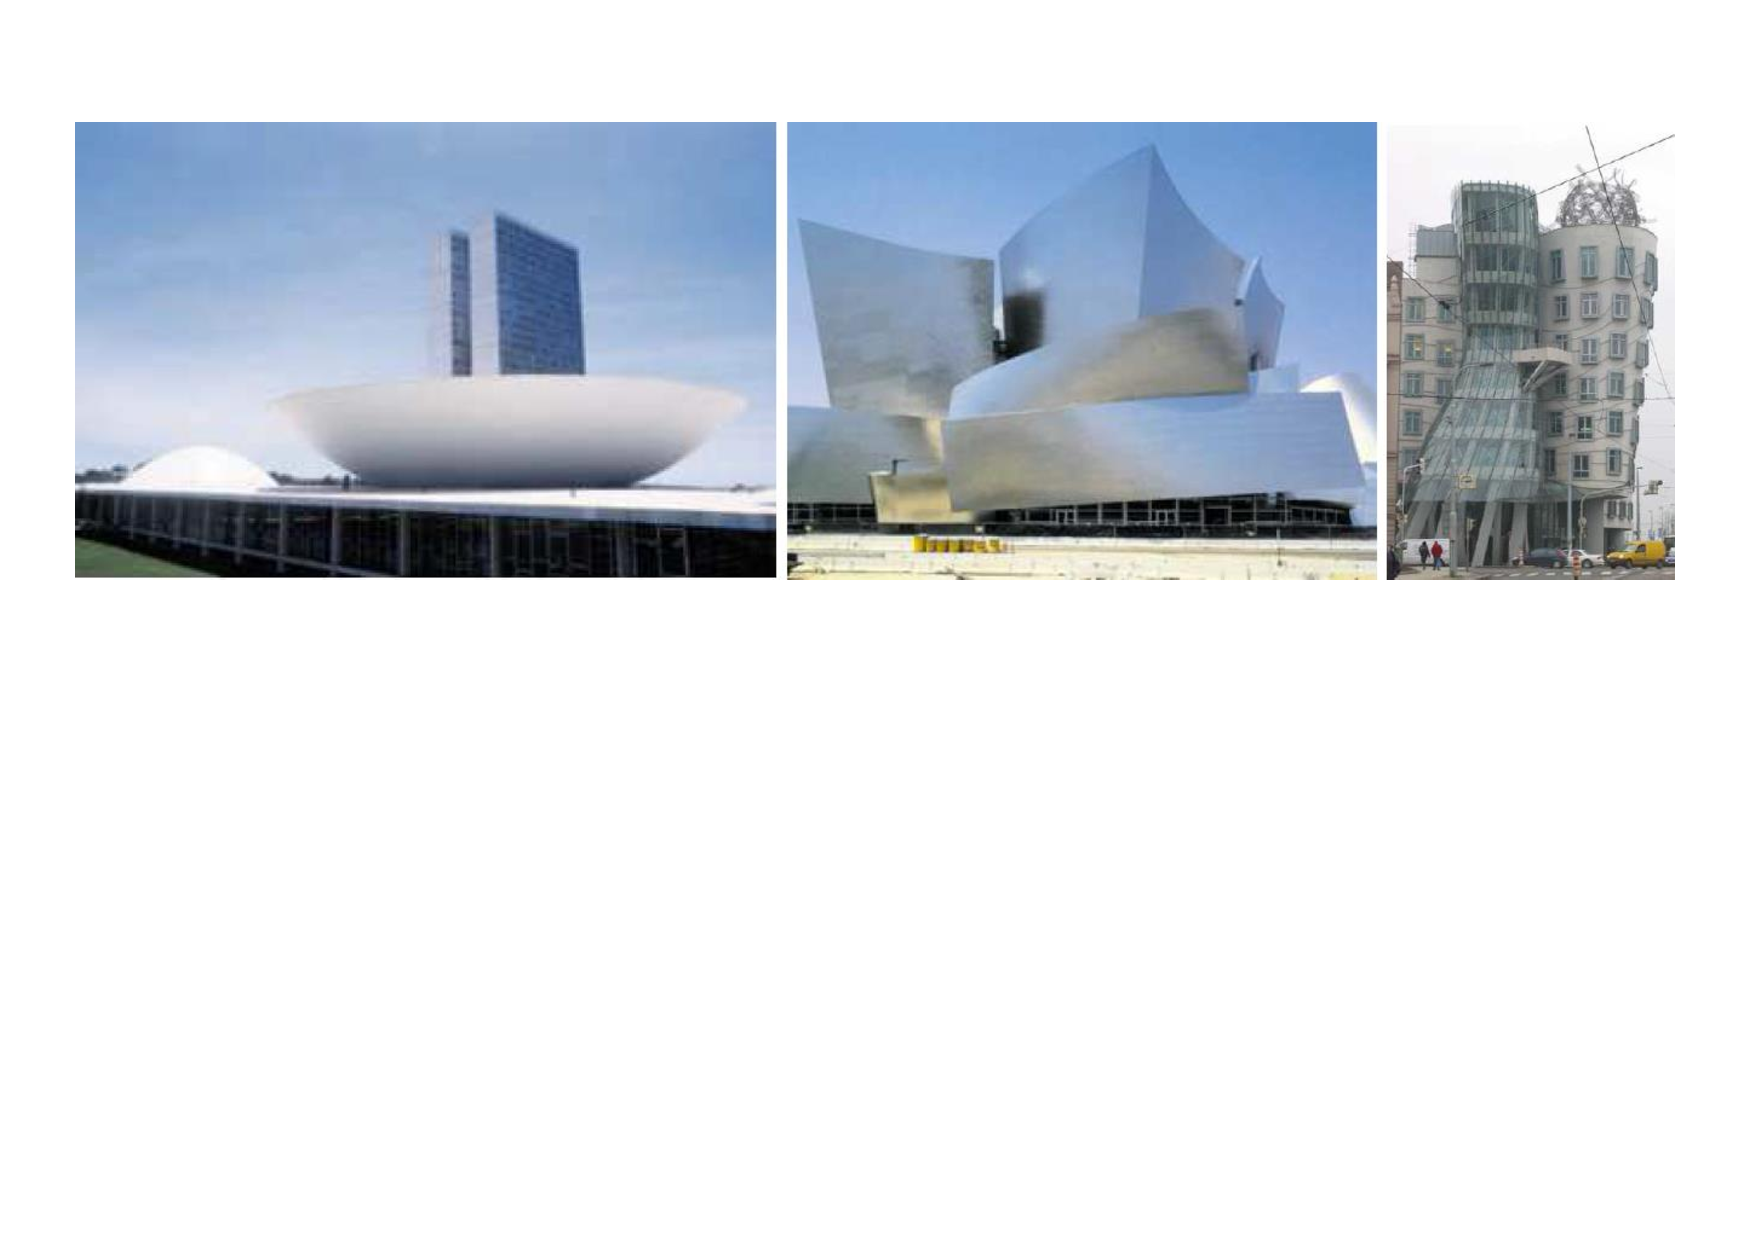
\includegraphics[width=1\textwidth]{images/postmoderne}
\subsection{Wichtige Schweizer Architekten}
Sehr viele Architekten in Rom und St. Petersburg waren Tessiner Architekten.
\subsubsection{Le Corbusier (Charles-Edouard Jeanneret-Gris) (1887- 1965)}
Seit 1917 in Paris tätig. Tätigkeit als Stadtplaner. Viele Entwürfe nicht berücksichtigt, da formelle Unzulänglichkeiten. Nähe zu totalitären Diktatoren um den Zweiten Weltkrieg. Diverse Wohnbauten und staatliche Gebäude konzipiert. Erfinder des Modulor (Proportionssystem um die Architektur mathematische zu ordnen).
\subsubsection{Mario Botta (*1943)}
Tessiner. Ausbildung zum Hochbauzeichner. Beachtet schlichte Formen. Setzt oft natürliche Materialien ein. Professor an der Universität der Italienischen Schweiz.
\subsubsection{Jacques Herzog (*1950) und Pierre de Meuron (*1950)}
Studium an der ETH Zürich. Bau von Sportstadien. Bau und Erneuerung diverser Museen.
\subsubsection{Peter Zumthor (*1943)}
Lehre als Möbelschreiner. Studium als Innenarchitekt und Architekt. Mitarbeiter der Denkmalpflege GR. Im Vordergrund steht bei ihm die im Bau verwendeten Materialien. Teilweise massive Kostenüberschreitungen.
\subsection{Die verschiedenen Kulturepochen – Kleidung}
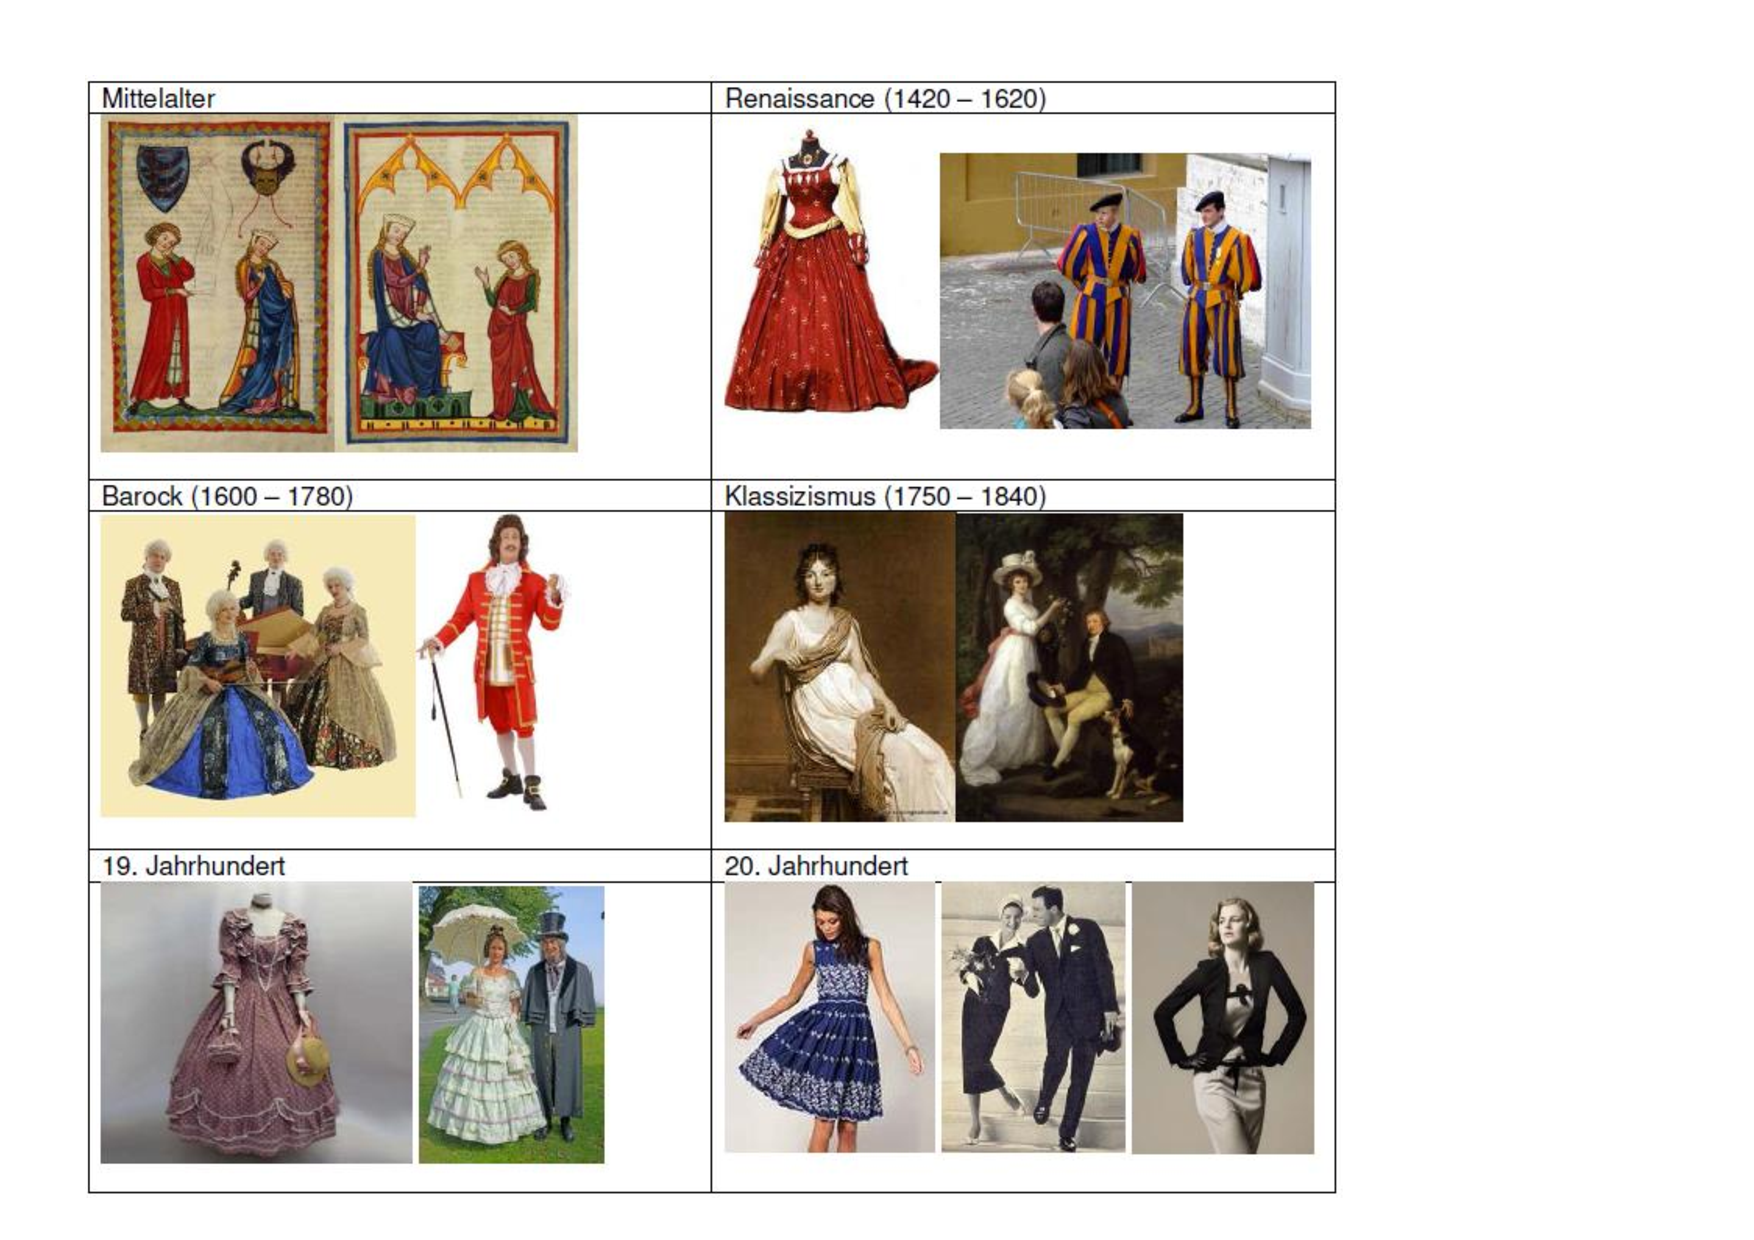
\includegraphics[width=1\textwidth]{images/kleidung}
\section{Technische Entwicklung in der Schweiz}
\subsection{Römische Zeit}
Übernahme der römischen Kultur und Technik. Strassen und öffentliche Gebäude. Bäder und Kanalisation. Kunstdenkmäler und gegenständliche Kunst.
\subsection{Mittelalter}
Kulturträger sind die Klöster (bspw. Saint Maurice, St. Gallen, Einsiedeln). Die bäuerliche Gesellschaft hinterliess wenig Spuren. Zwei \glqq Erfindungen\grqq werden aber sehr wichtig und haben gewaltige Auswirkungen für und auf die Schweiz:
\subsubsection{Gotthardpass}
Ab ca. 1230 wird der Gotthardpass dank der Begehbarmachung der Schöllenenschlucht zu einer wichtigen Alpentransversale. Die Inner-Schweiz wird von einer politisch, geographischen und wirtschaftlichen Sackgasse zu einer zentralen europäischen Achse. Diverse Herrscher versuchen dieses nun strategisch wichtige Gebiet in ihren Einfluss zu bekommen, bspw. die Habsburger. Dank Pass und Solddienst können sich die Talschaften freikaufen und werden reichsunmittelbar. \vspace{-0.5cm}
\subsubsection{Halbarte}
Dank einer neuen Waffe, der Halbarte, können die Eidgenossen ihre Selbstbestimmung gegenüber den adligen Familien verteidigen. Eidgenössische Fusssoldaten sind nun den Ritterheeren überlegen. Solddienst wird für Eidgenossen zu einer Haupterwerbsquelle. Die Eidgenossenschaft wird für Städte attraktiv – Vergrösserung der Bündnisse. \vspace{-0.5cm}
\subsection{Zeit der Renaissance und der Aufklärung}
Keine technischen Entwicklungen, da die Zünfte diese verbieten. Während der Aufklärung Versuche die Landwirtschaft zu verbessern – Kleinjogg (1716 – 1785). Beginn der Uhrenindustrie in der Westschweiz, dank den aus Frankreich fliehenden Hugenotten. Zentrum der Uhrenindustrie wird Genf. \vspace{-0.5cm}
\subsection{Ab 1804 erste Versuche zur Industrialisierung}
Für die frühe Industrialisierung der Schweiz sprach eine freie Marktwirtschaft, ein liberaler Staat, gut ausgebildete Menschen, tiefe Löhne da ein Arbeiterüberschuss, geographische Kleinheit, Föderalismus und das Milizsystem.
\begin{citemize}
\item Baumwollweberei und Druckerei (Bsp. Glarner Tüechli)
\item Mechanisch Spinnerei und Webmaschinen (Bsp. Webstühle von Honegger, Maschinen von Sulzer / Escher-Wyss)
\item Nahrungsmittelindustrie (Bsp. Nestle, Lindt, Cailler, Sucher, Peter)
\item Schuhindustrie
\item Uhrenindustrie (Bsp. Genf, IWC, Rolex, Tissot, (Jurabogen))
\end{citemize} \vspace{-0.5cm}
\subsubsection{Industrialisierung in der Schweiz}
Zeitliche Verhältnisse?\\
Früh, Beginn 1. Hälfte des 19. Jahrhunderts\\
Gründe dafür?\\
Freie Marktwirtschaft, liberaler Staat; Bevölkerungsüberschuss – tiefe Löhne; Willige und gut ausgebildete Bevölkerung\\
Wie beginnt die Industrialisierung?\\
Textilindustrie, führt zu: Maschinenindustrie; Chemische Industrie\\
In der Schweiz spielte die Dampfmaschine keine grosse Rolle, da keine Kohle vorhanden ist, jedoch Flüsse mit starkem Gefälle. \\
Wichtige Namen in der Maschinenindustrie:\\
BBC (heute ABB): Elektroinstallation\\
Sulzer, Winterthur: Pumpen und Turbinen / Lokomotiven\\
Honegger, Siebnen: Webstühle \vspace{-0.5cm}
\subsubsection{Nahrungsindustrie}
Hauptprodukte: Hartkäse, Schokolade\\
Wichtige Persönlichkeiten: Suchard, Cailler, Lindt \vspace{-0.5cm}
\subsubsection{Soziale Frage (siehe 5.2)}
Materielle \& rechtliche Situation während der zweiten Industriellen Revolution.\\
Lösungen (siehe 5.3):\\
Staat: Arbeits- und Sozial-Gesetz\\
Arbeiter: Gewerkschaften und Parteien\\
Arbeitgeber: Schule, Krankenhäuser, usw.\\
Philosophen: neue Ideologien\\
Durch die technische Entwicklung (Fortschritte) verkleinert sich die Soziale Frage, da anspruchsvolle Maschinen gut ausgebildete und ausgeruhte Arbeiter verlangt.
\end{document}
